% !TeX program = pdflatex
% !TeX root = main.tex
\documentclass[12pt, a4paper, oneside]{article}
\usepackage[utf8]{inputenc}
\usepackage[T5]{fontenc}
\usepackage[vietnamese]{babel}
\usepackage[top = 2.5cm, bottom = 2.5cm, left = 1.5cm, right = 1cm]{geometry}
\usepackage{amsmath,amsfonts,amssymb}
\usepackage{indentfirst,enumitem}
\usepackage{graphicx}
\let\originalincludegraphics\includegraphics
\renewcommand{\includegraphics}[2][]{%
    \IfFileExists{#2}{\originalincludegraphics[#1]{#2}}{%
        \fbox{\parbox[c][3cm][c]{0.8\linewidth}{\centering Missing image: \texttt{\detokenize{#2}}}}%
    }%
}
\usepackage{multicol}
\usepackage{multirow}
\usepackage{setspace}
\usepackage{hyperref}
\usepackage{listings}
\usepackage{tabularx}
\usepackage{hyperref}
\usepackage{xcolor}
\usepackage{scrextend}
\usepackage{comment}
\usepackage{soul}
\usepackage{tipa}
\usepackage{subfigure}
\usepackage{caption}
\usepackage{booktabs}
\usepackage{array}
\usepackage{fancyhdr}
\usepackage{algorithm2e}
\usepackage{float}
\usepackage[most]{tcolorbox}
\usepackage{pdfpages}
\usepackage{import}
\graphicspath{ {figures/} }
\usepackage{titlesec}
\usepackage{listingsutf8}

\lstset{
    inputencoding=utf8,
    extendedchars=true,
    literate=
        {á}{{\'a}}1 {à}{{\`a}}1 {ả}{{\?a}}1 {ã}{{\~a}}1 {ạ}{{\.a}}1
}

\titleformat{\paragraph}
{\normalfont\normalsize\bfseries}
{\theparagraph}{1em}{}

\titlespacing*{\paragraph}
{0pt}{3ex plus 1ex minus .2ex}{1em}
\usepackage{float}
\usepackage{tikz}
\usetikzlibrary{calc, positioning, shapes.geometric}
\usetikzlibrary{circuits.logic.US, circuits.logic.IEC}

\captionsetup[figure]{labelfont=bf, textfont=it, font=small}

\hypersetup{
    colorlinks=true,
    linkcolor=black,
    filecolor=magenta,      
    urlcolor=black,
    pdftitle={TKHTN},
    pdfpagemode=FullScreen,
}

%\changefontsizes{13pt}
\renewcommand\thesection{\arabic{section}.}
\renewcommand\thesubsection{\arabic{section}.\arabic{subsection}}

\pagestyle{fancy}
\fancypagestyle{plain}{\fancyhf{}}
\fancyhead[r]{\textit{Khoa Điện - Điện tử}}
%\fancyhead[c]{\bfseries DSP}
\fancyhead[l]{\textit{Thiết kế vi mạch}}
\renewcommand{\headrulewidth}{0.2pt}
\setlength{\headheight}{10pt}


\def\mathrlap{\mathpalette\mathrlapinternal} 
\def\mathclap{\mathpalette\mathclapinternal}
\def\mathllapinternal#1#2{\llap{$\mathsurround=0pt#1{#2}$}}
\def\mathrlapinternal#1#2{\rlap{$\mathsurround=0pt#1{#2}$}}

%CHÈN ẢNH
\usepackage{pgfplots}
\pgfplotsset{compat=1.15}
\usepackage{mathrsfs}
\usetikzlibrary{arrows}
\usetikzlibrary[patterns]

%New colors defined below
\definecolor{codegreen}{rgb}{0,0.6,0}
\definecolor{codegray}{rgb}{0.5,0.5,0.5}
\definecolor{codepurple}{rgb}{0.58,0,0.82}
\definecolor{backcolour}{rgb}{0.95,0.95,0.92}

\input{verilogstyle}
\setlength{\headheight}{14.94pt}
\begin{document}

\thispagestyle{empty}
% Định nghĩa macro vẽ ký hiệu tam giác cho chân Clock
\def\clktriangle#1#2{
    \draw (#1, #2) ++(0, 0.15) -- ++(0.2, -0.15) -- ++(-0.2, -0.15);
}
\begin{titlepage}
%\SetWatermarkText{\includegraphics[width = 0.97\paperwidth,
%height = 0.97\paperheight]{bia.png}}
%\SetWatermarkAngle{0} 
%\SetWatermarkText{\includegraphics[scale=1]{hust.png}}
%\SetWatermarkAngle{0} 
\begin{tikzpicture}[remember picture,overlay,inner sep=0,outer sep=0]
     \draw[blue!70!black,line width=4pt] ([xshift=-1.5cm,yshift=-2cm]current page.north east) coordinate (A)--([xshift=1.5cm,yshift=-2cm]current page.north west) coordinate(B)--([xshift=1.5cm,yshift=2cm]current page.south west) coordinate (C)--([xshift=-1.5cm,yshift=2cm]current page.south east) coordinate(D)--cycle;

     \draw ([yshift=0.5cm,xshift=-0.5cm]A)-- ([yshift=0.5cm,xshift=0.5cm]B)--
     ([yshift=-0.5cm,xshift=0.5cm]B) --([yshift=-0.5cm,xshift=-0.5cm]B)--([yshift=0.5cm,xshift=-0.5cm]C)--([yshift=0.5cm,xshift=0.5cm]C)--([yshift=-0.5cm,xshift=0.5cm]C)-- ([yshift=-0.5cm,xshift=-0.5cm]D)--([yshift=0.5cm,xshift=-0.5cm]D)--([yshift=0.5cm,xshift=0.5cm]D)--([yshift=-0.5cm,xshift=0.5cm]A)--([yshift=-0.5cm,xshift=-0.5cm]A)--([yshift=0.5cm,xshift=-0.5cm]A);


     \draw ([yshift=-0.3cm,xshift=0.3cm]A)-- ([yshift=-0.3cm,xshift=-0.3cm]B)--
     ([yshift=0.3cm,xshift=-0.3cm]B) --([yshift=0.3cm,xshift=0.3cm]B)--([yshift=-0.3cm,xshift=0.3cm]C)--([yshift=-0.3cm,xshift=-0.3cm]C)--([yshift=0.3cm,xshift=-0.3cm]C)-- ([yshift=0.3cm,xshift=0.3cm]D)--([yshift=-0.3cm,xshift=0.3cm]D)--([yshift=-0.3cm,xshift=-0.3cm]D)--([yshift=0.3cm,xshift=-0.3cm]A)--([yshift=0.3cm,xshift=0.3cm]A)--([yshift=-0.3cm,xshift=0.3cm]A);

   \end{tikzpicture}
\begin{center}
    \vspace{7pt}
        \textbf{ĐẠI HỌC QUỐC GIA THÀNH PHỐ HỒ CHÍ MINH}
    
    \vspace{7pt}
    \textbf{TRƯỜNG ĐẠI HỌC BÁCH KHOA}
    
    \vspace{7pt}
    \textbf{KHOA ĐIỆN - ĐIỆN TỬ}
\end{center}
\vspace{10pt}
\begin{center}
    
\includegraphics[scale=0.3]{HCMUT.png}
    \vspace{10pt}
\end{center}

\begin{center}
    \fontsize{18pt}{17pt}\selectfont 
    \textbf{BÁO CÁO THÍ NGHIỆM}

    \textbf{MÔN:  THIẾT KẾ VI MẠCH}
\end{center}
\begin{center}
    \fontsize{15pt}{17pt}\selectfont 
    \textbf{\textrm{LAB 5: Circuit Design for Basic Standard Cells }}
\end{center}

\begin{center}
    \vspace{15pt}
    \textbf{Lớp: L03 - NHÓM: 5}
    
    \textbf{GVHD: ThS. Nguyễn Trung Hiếu}
\end{center}

\vspace{10pt}

\begin{table}[h!]
\centering
\begin{tabular}{|c|c|c|}
\hline
\textbf{MSSV} & \textbf{Họ và tên} & \textbf{Tỉ lệ phân công} \\ \hline
2311267 & Vũ Nhật Huy & 100\% \\ \hline
2313355 & Nguyễn Minh Thuận & 100\% \\ \hline
2313222 & Thái Đức Thiên & 100\% \\ \hline
\end{tabular}
\end{table}
\vfill
\centerline{\bf Thành phố Hồ Chí Minh, tháng 5 năm 2026}

\vspace{1cm}
\end{titlepage}
\newpage
\tableofcontents
\newpage

% =================================================================
% EXPERIMENT 1: CMOS INVERTER
% =================================================================
\section{Experiment 1: Circuit Design for a CMOS NOT Logic Gate}

\subsection{Mục tiêu}
Thực hiện thiết kế nguyên lý (Schematic), tạo biểu tượng (Symbol) và mô phỏng (DC, Transient) cho cổng NOT sử dụng công nghệ GPDK045.

\subsection{Bảng trạng thái và Nguyên lý hoạt động}
\begin{itemize}
    \item \textbf{Bảng chân trị (Truth Table):}
    \begin{center}
        \begin{tabular}{|c|c|}
        \hline
        Input (IN) & Output (OUT) \\ \hline
        0 & 1 \\ \hline
        1 & 0 \\ \hline
        \end{tabular}
    \end{center}
    \item \textbf{Nguyên lý hoạt động:} Mô tả vùng hoạt động của NMOS và PMOS khi ngõ vào ở mức Logic 0 (PMOS dẫn - vùng tuyến tính, NMOS ngắt) và Logic 1 (NMOS dẫn, PMOS ngắt).
\end{itemize}

\subsection{Thiết kế Schematic và Symbol}
\textbf{Sizing:} NMOS ($W/L = 120n/45n$, Finger=2), PMOS ($W/L = 120n/45n$, Finger=2).

% Chèn hình Schematic và Symbol của INV
\begin{figure}[H]
    \centering
    \subfigure[Schematic của Inverter]{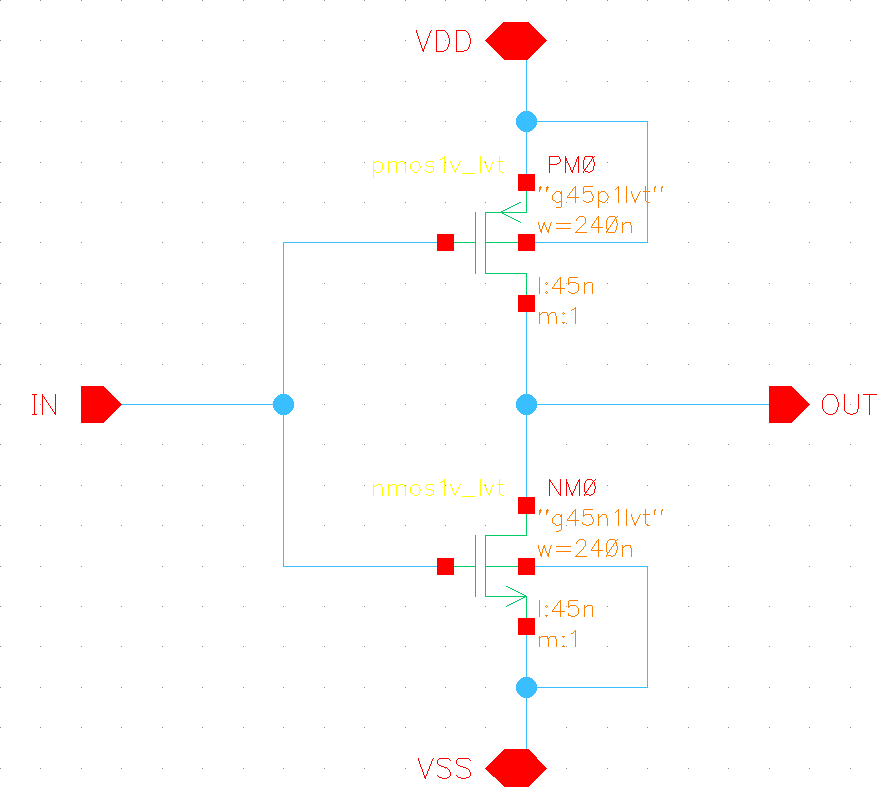
\includegraphics[width=0.45\textwidth]{inv_schematic.png}}
    \subfigure[Symbol của Inverter]{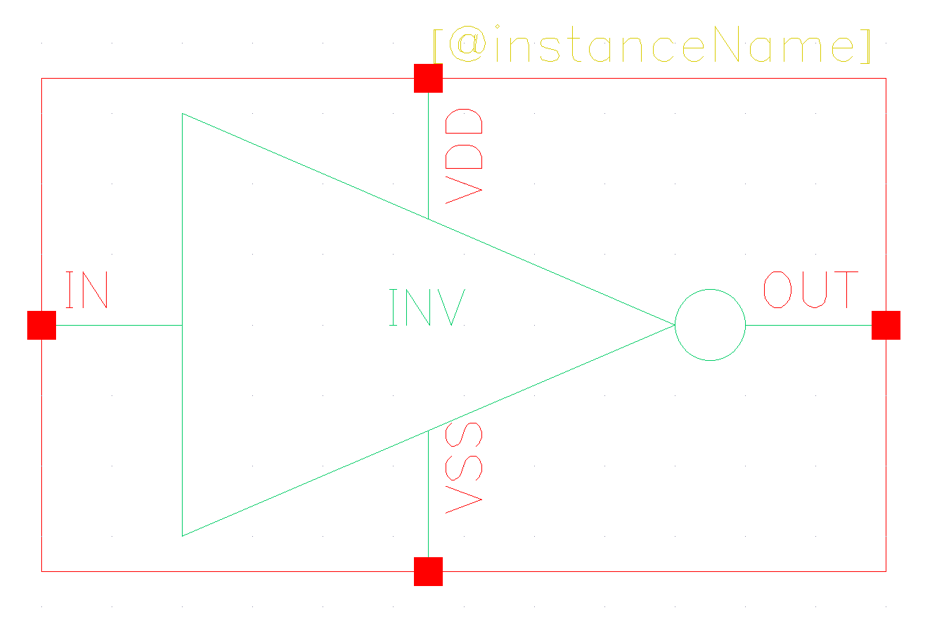
\includegraphics[width=0.45\textwidth]{inv_symbol.png}}
    \caption{Thiết kế nguyên lý cổng Inverter}
\end{figure}

\subsection{Mô phỏng DC Analysis}
\textbf{Thiết lập Testbench:} Sử dụng nguồn ramp từ 0V đến 1V.
\begin{figure}[H]
    \centering
    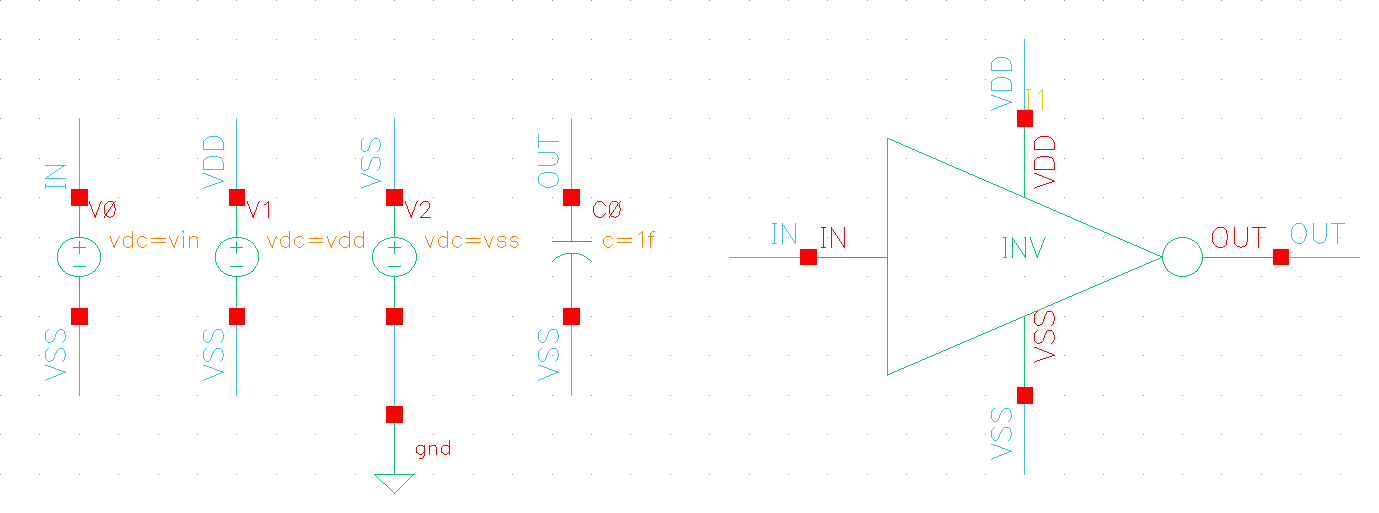
\includegraphics[width=0.7\textwidth]{inv_dc_testbench.png}
    \caption{Testbench mô phỏng DC cổng Inverter}
\end{figure}

\textbf{Kết quả mô phỏng VTC (Voltage Transfer Characteristics):}
% Chèn hình đặc tuyến VTC và cách tìm VIH, VIL, VOH, VOL, VM từ slide
\begin{figure}[H]
    \centering
    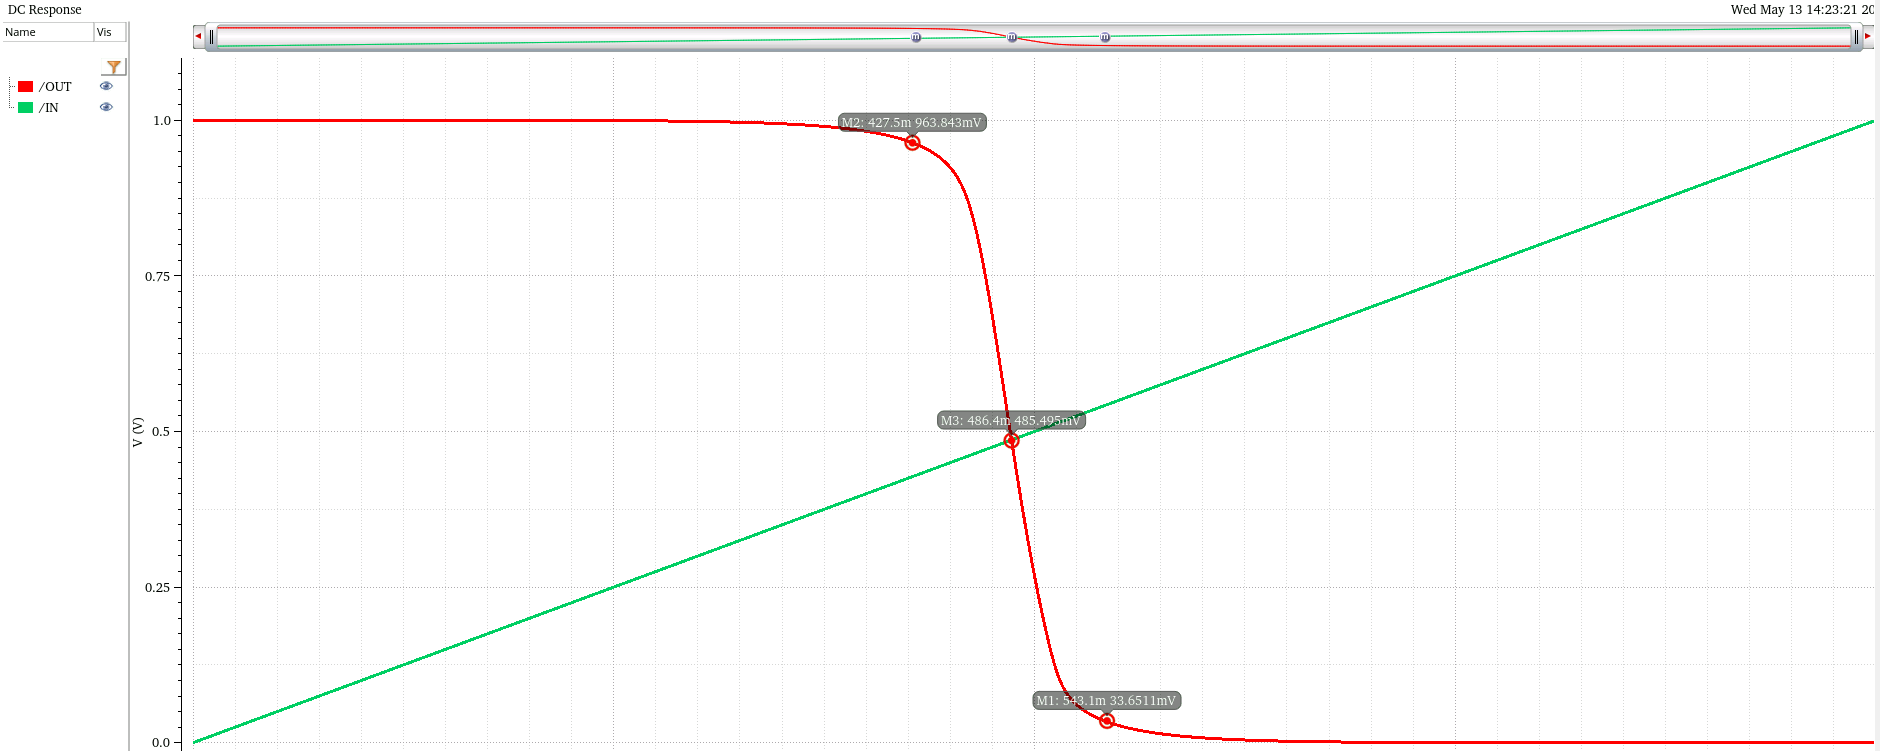
\includegraphics[width=0.8\textwidth]{inv_dc_response.png}
    \caption{Đặc tuyến chuyển tiếp điện áp VTC của cổng Inverter}
\end{figure}

\textbf{Bảng giá trị ngõ ra theo ngõ vào (Step 0.1V):}
\begin{center}
    \begin{tabular}{|c|c|c|c|c|c|c|c|c|c|c|}
    \hline
    $V_{in}$ (V) & 0.1 & 0.2 & 0.3 & 0.4 & 0.5 & 0.6 & 0.7 & 0.8 & 0.9 & 1.0 \\ \hline
    $V_{out}$ (V) & 0.99 & 0.99 & 0.99 & 0.98 & 0.26 & 0.007 & 0.78 & 0.0007 & 0.00006 & 0.000003 \\ \hline
    \end{tabular}
\end{center}

\textbf{Các thông số Noise Margin:} Từ đồ thị xác định:
\begin{itemize}
    \item $V_{IL}, V_{IH}, V_{OL}, V_{OH}$
    \item Điểm trung điểm $V_M$
\end{itemize}

\subsection{Mô phỏng Transient Analysis}
\textbf{Thiết lập thông số vpulse:} Period = 2ns, Pulse Width = 1ns, $t_r = t_f = 1ps$.
\begin{figure}[H]
    \centering
    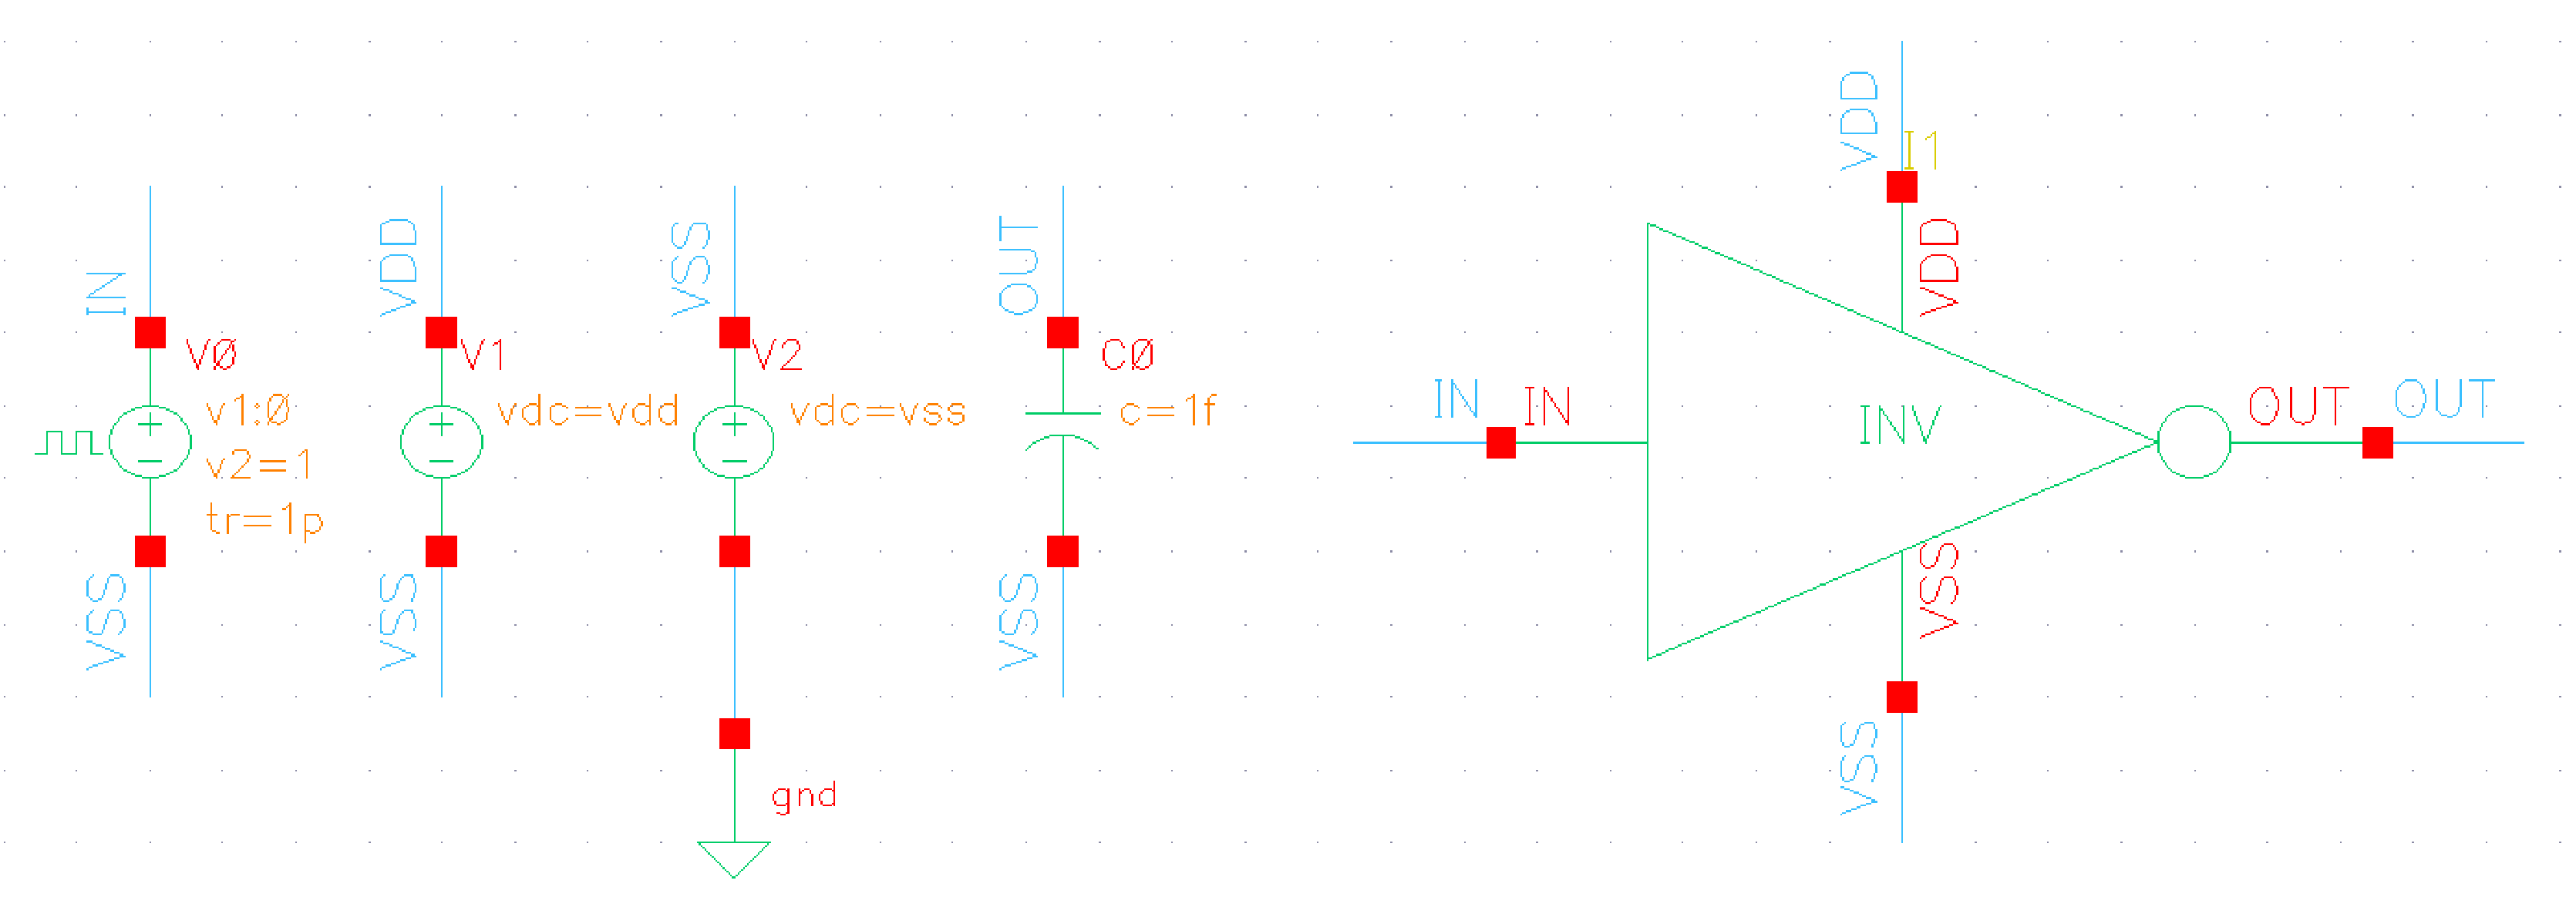
\includegraphics[width=0.7\textwidth]{inv_transient_testbench.png}
    \caption{Testbench mô phỏng Transient cổng Inverter}
\end{figure}

\textbf{Kết quả dạng sóng ngõ vào/ngõ ra:}
\begin{figure}[H]
    \centering
    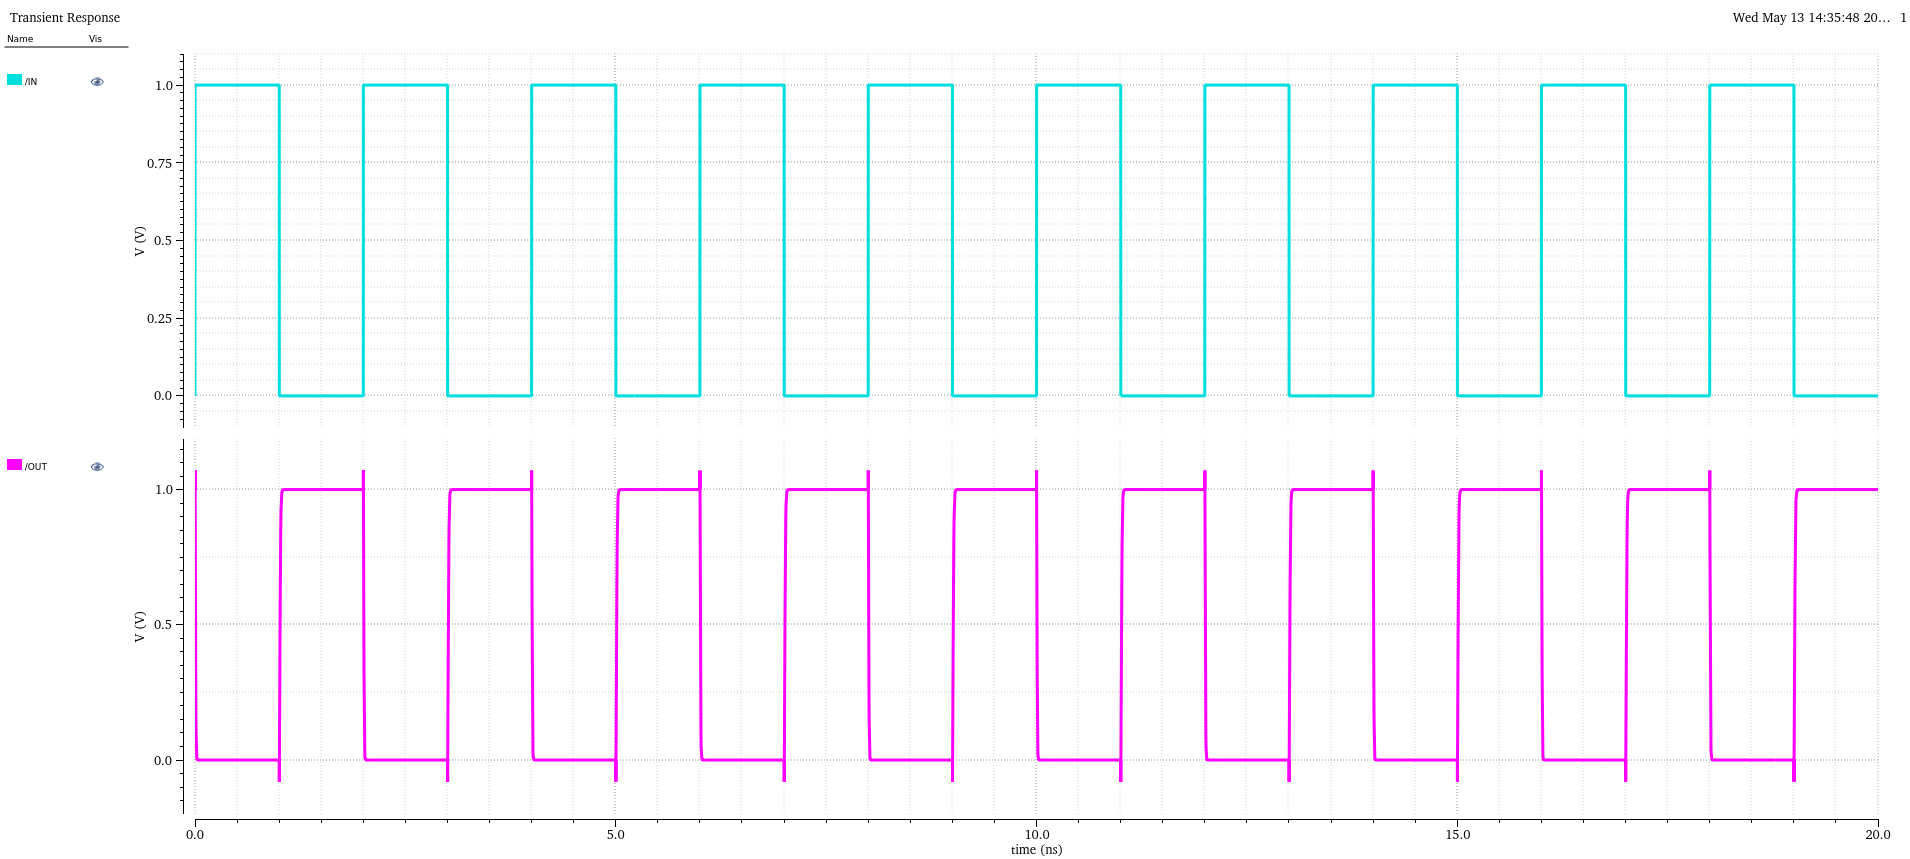
\includegraphics[width=0.8\textwidth]{inv_waveforms.png}
    \caption{Dạng sóng ngõ vào và ngõ ra của cổng Inverter}
\end{figure}

\textbf{Kết quả đo đạc thời gian và công suất:}
% Chèn các hình đo trise, tfall, tpdr, tpdf, tpd và công suất từ slide
\begin{figure}[H]
    \centering
    \subfigure[Đo $t_{rise}$]{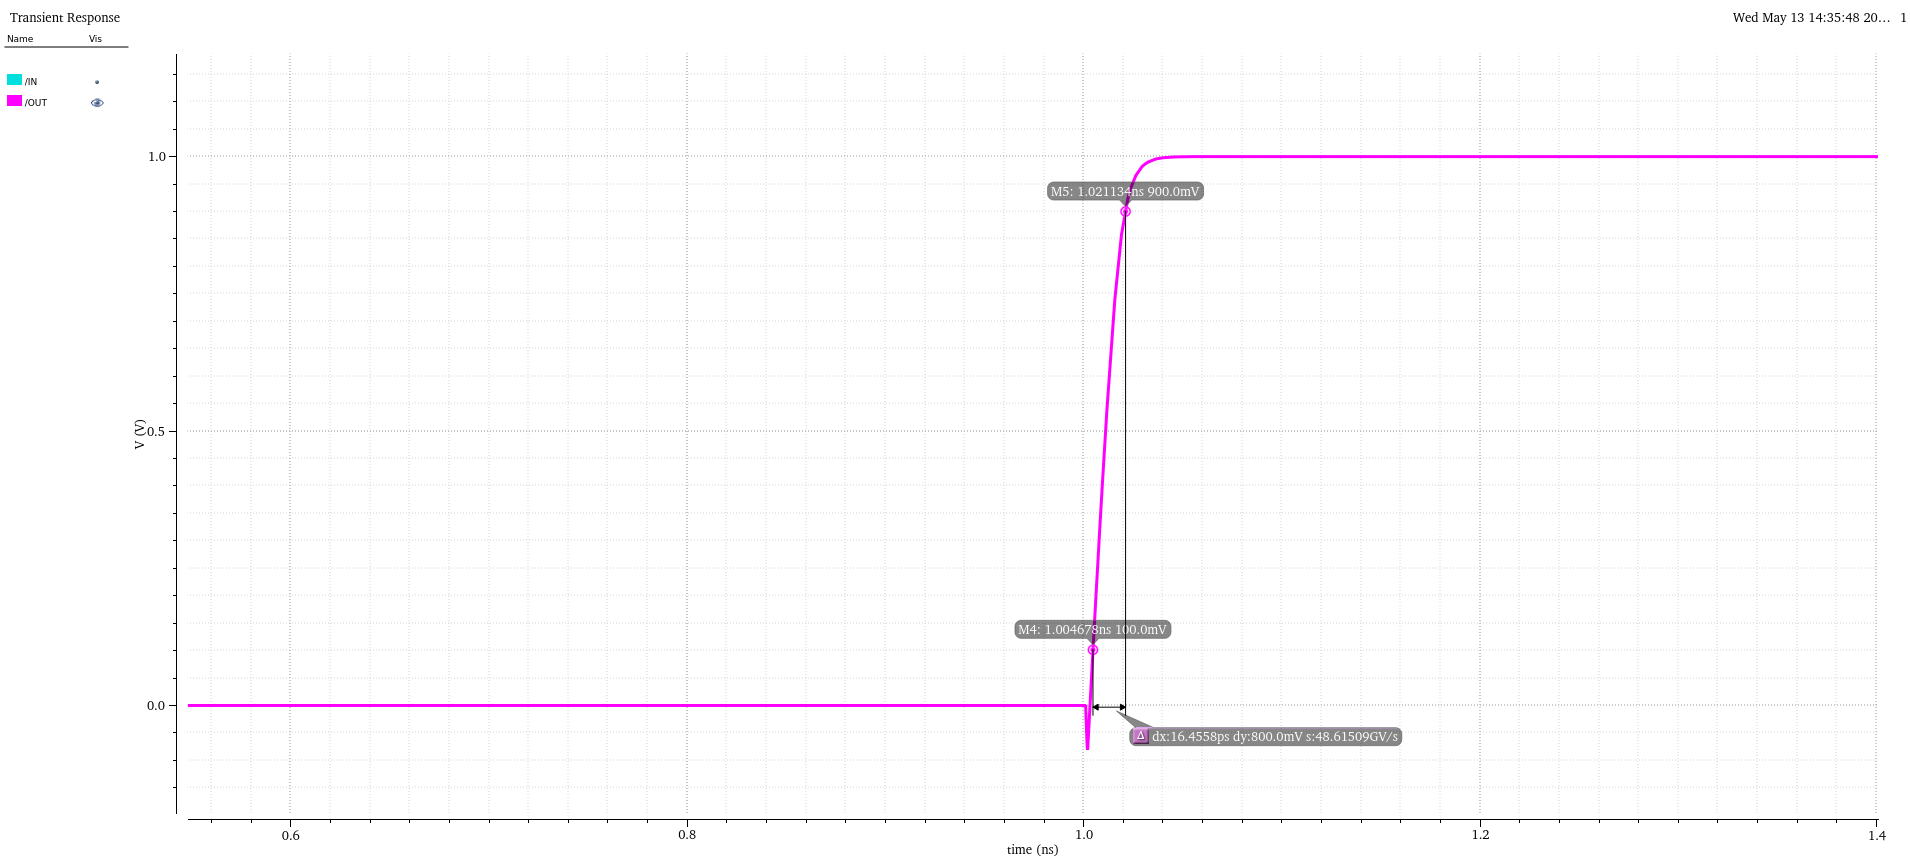
\includegraphics[width=0.5\textwidth]{inv_trise.png}}
    \subfigure[Đo $t_{fall}$]{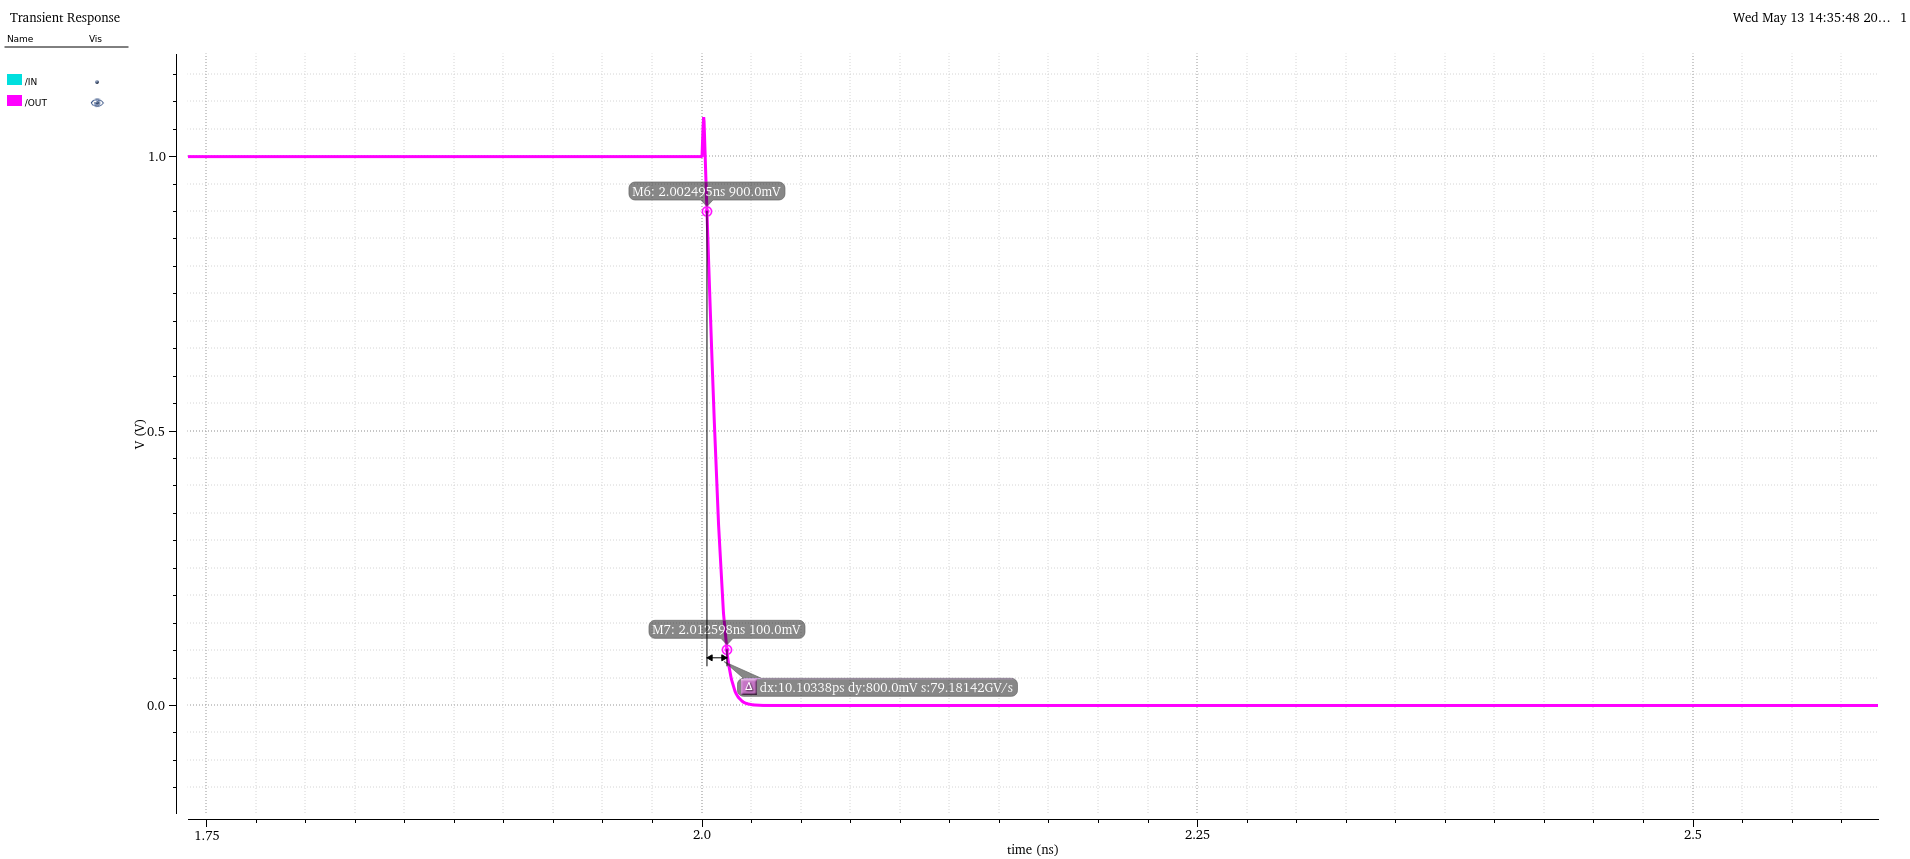
\includegraphics[width=0.5\textwidth]{inv_tfall.png}}
    \subfigure[Đo $t_{pdr}$]{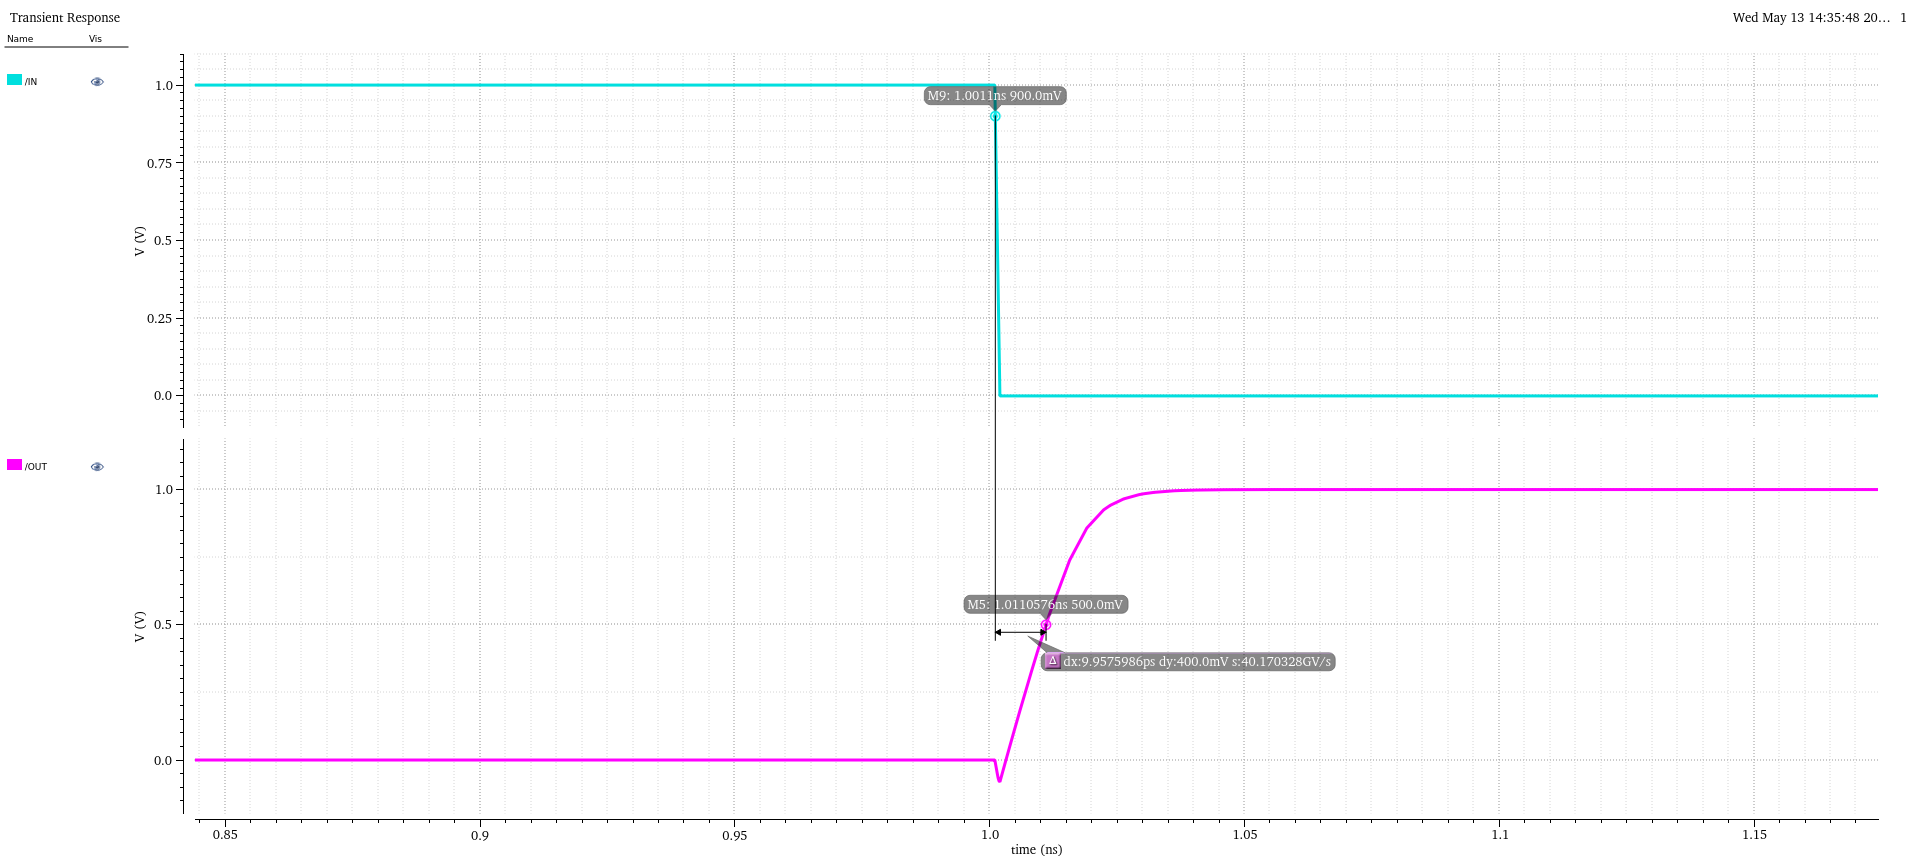
\includegraphics[width=0.5\textwidth]{inv_tpdr.png}}
\end{figure}
\begin{figure}[H]
    \centering
    \subfigure[Đo $t_{pdf}$]{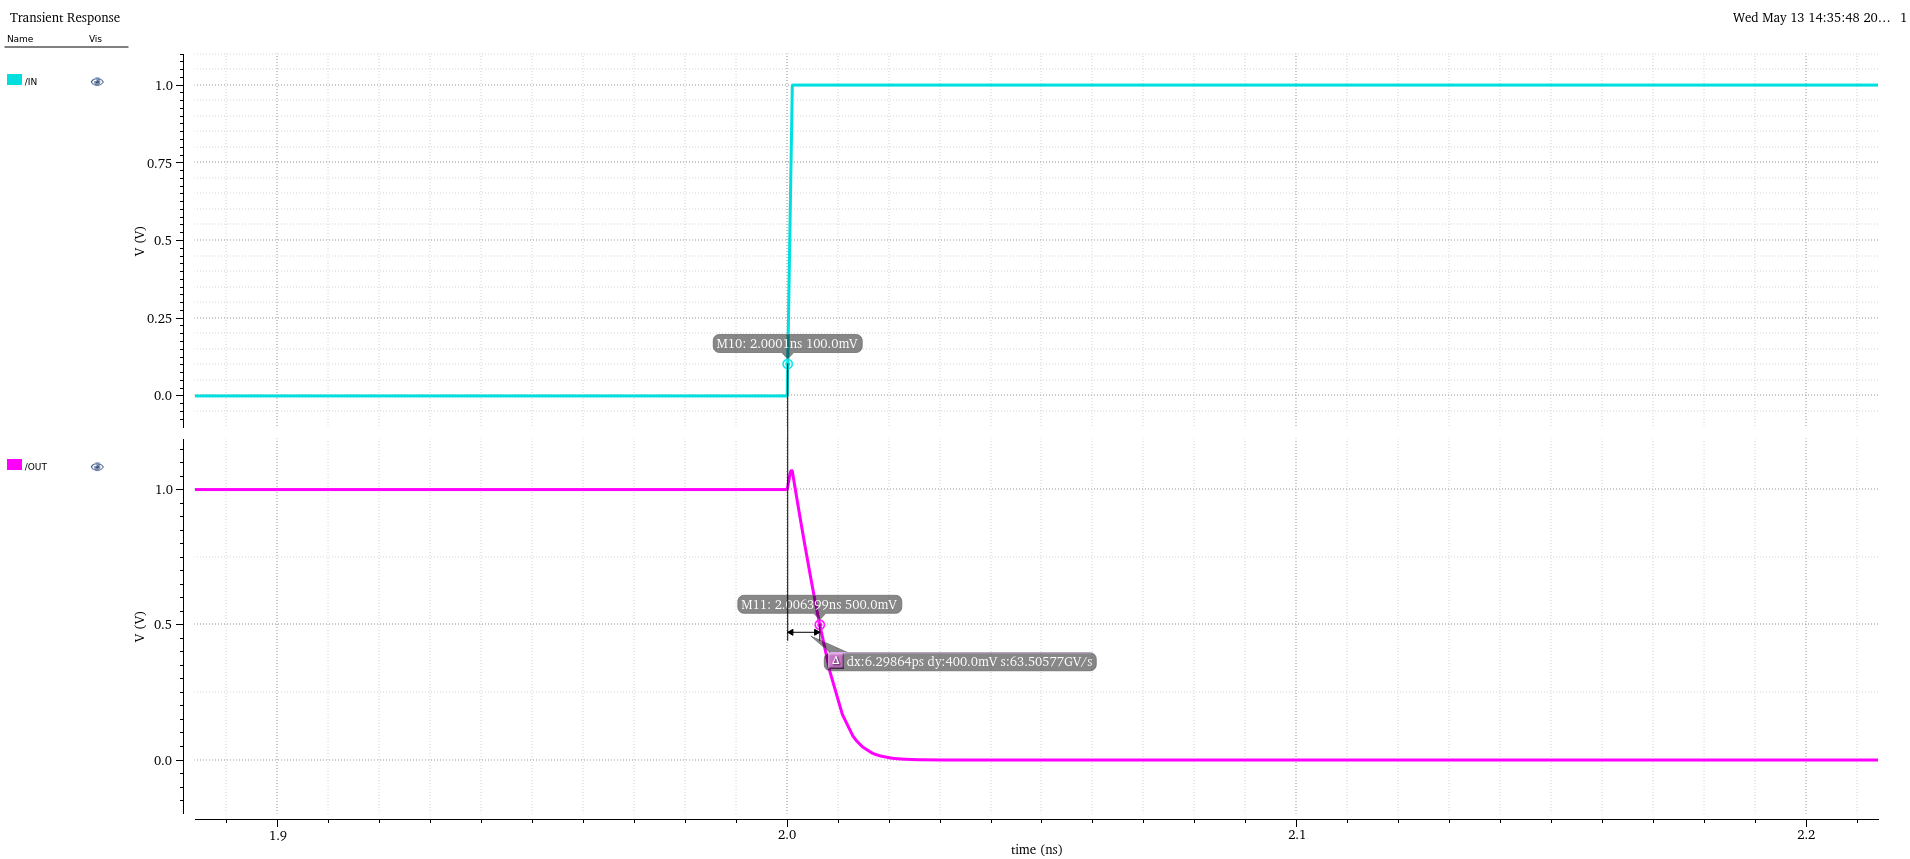
\includegraphics[width=0.5\textwidth]{inv_tpdf.png}}
    \subfigure[Đo $t_{pd}$]{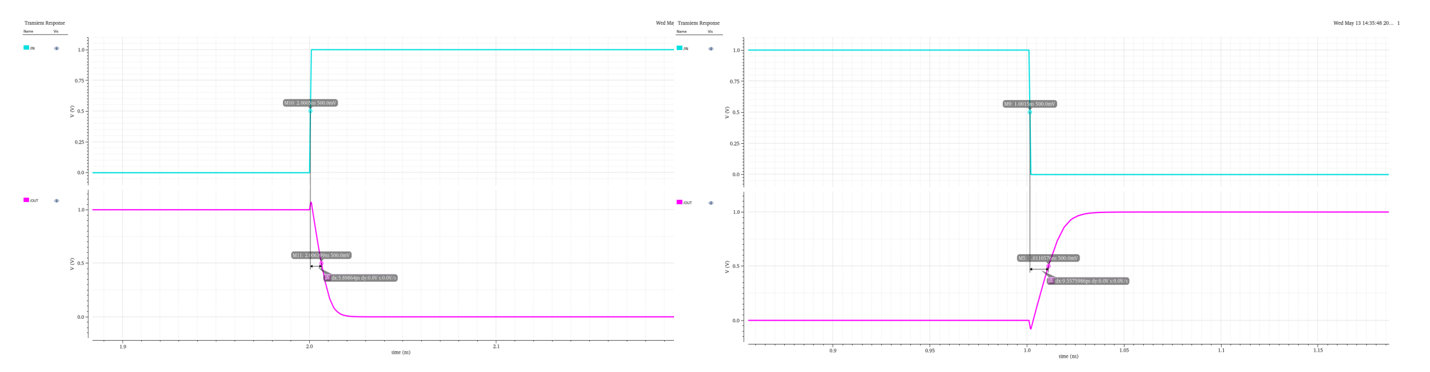
\includegraphics[width=0.5\textwidth]{inv_tpd.png}}
\end{figure}

\textbf{Đo công suất (Static and Dynamic Power):}
\begin{figure}[H]
    \centering
    \subfigure[Static Power ($V_{in}=0$)]{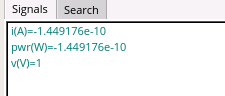
\includegraphics[width=0.5\textwidth]{inv_static_pwr_0.png}}
    \subfigure[Static Power ($V_{in}=1$)]{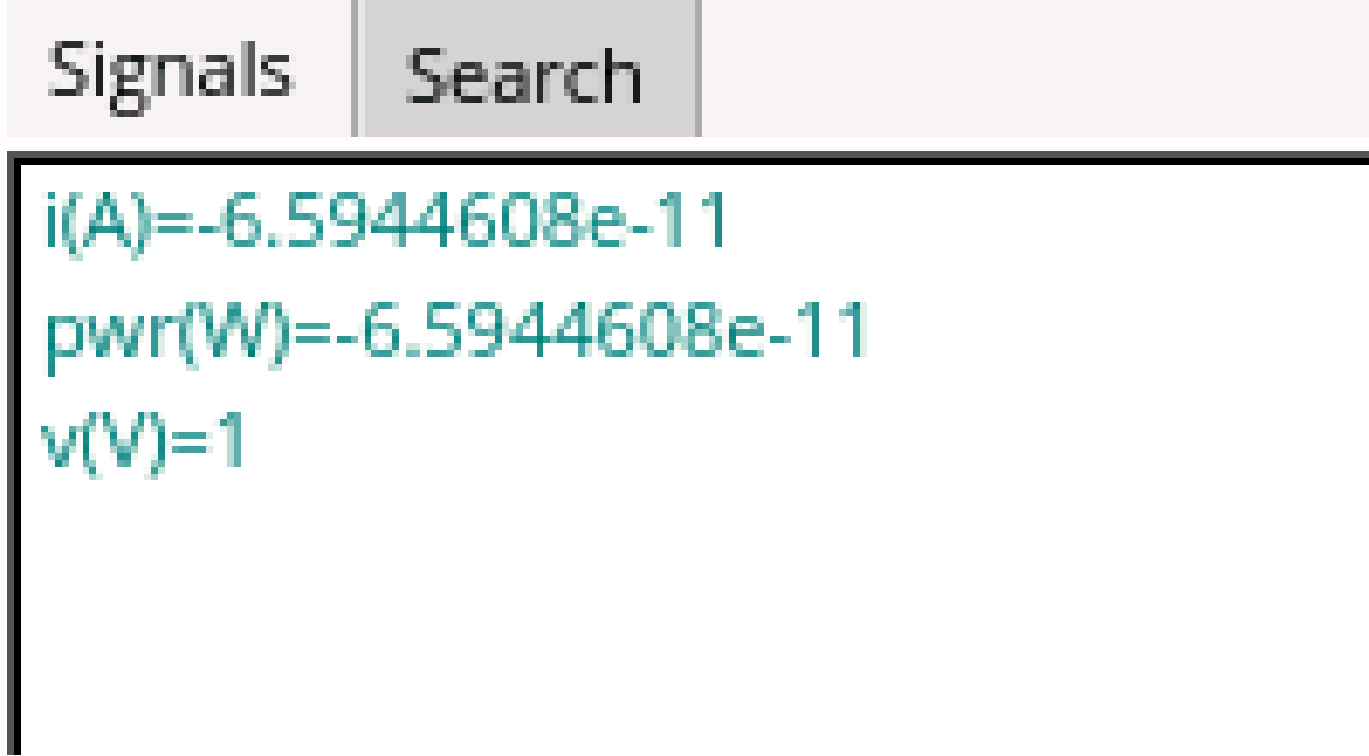
\includegraphics[width=0.5\textwidth]{inv_static_pwr_1.png}}
    \subfigure[Dynamic Power]{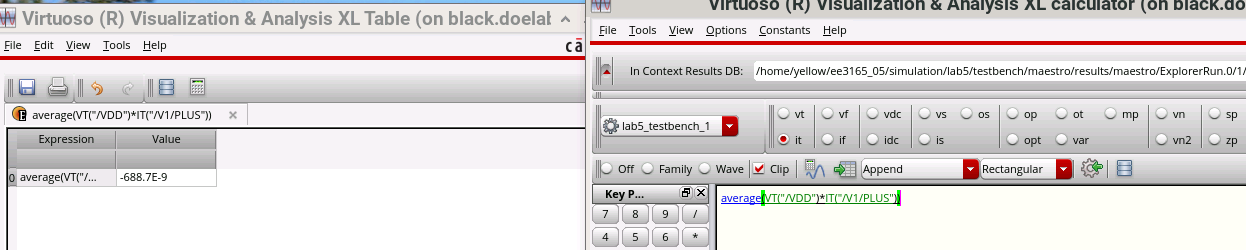
\includegraphics[width=0.5\textwidth]{inv_dynamic_pwr.png}}
\end{figure}

\subsection{Hiệu chỉnh kích thước (Adjust $V_M = V_{DD}/2$)}
Giải thích việc tăng Width của PMOS để bù độ linh động hạt tải thấp.
\begin{figure}[H]
    \centering
    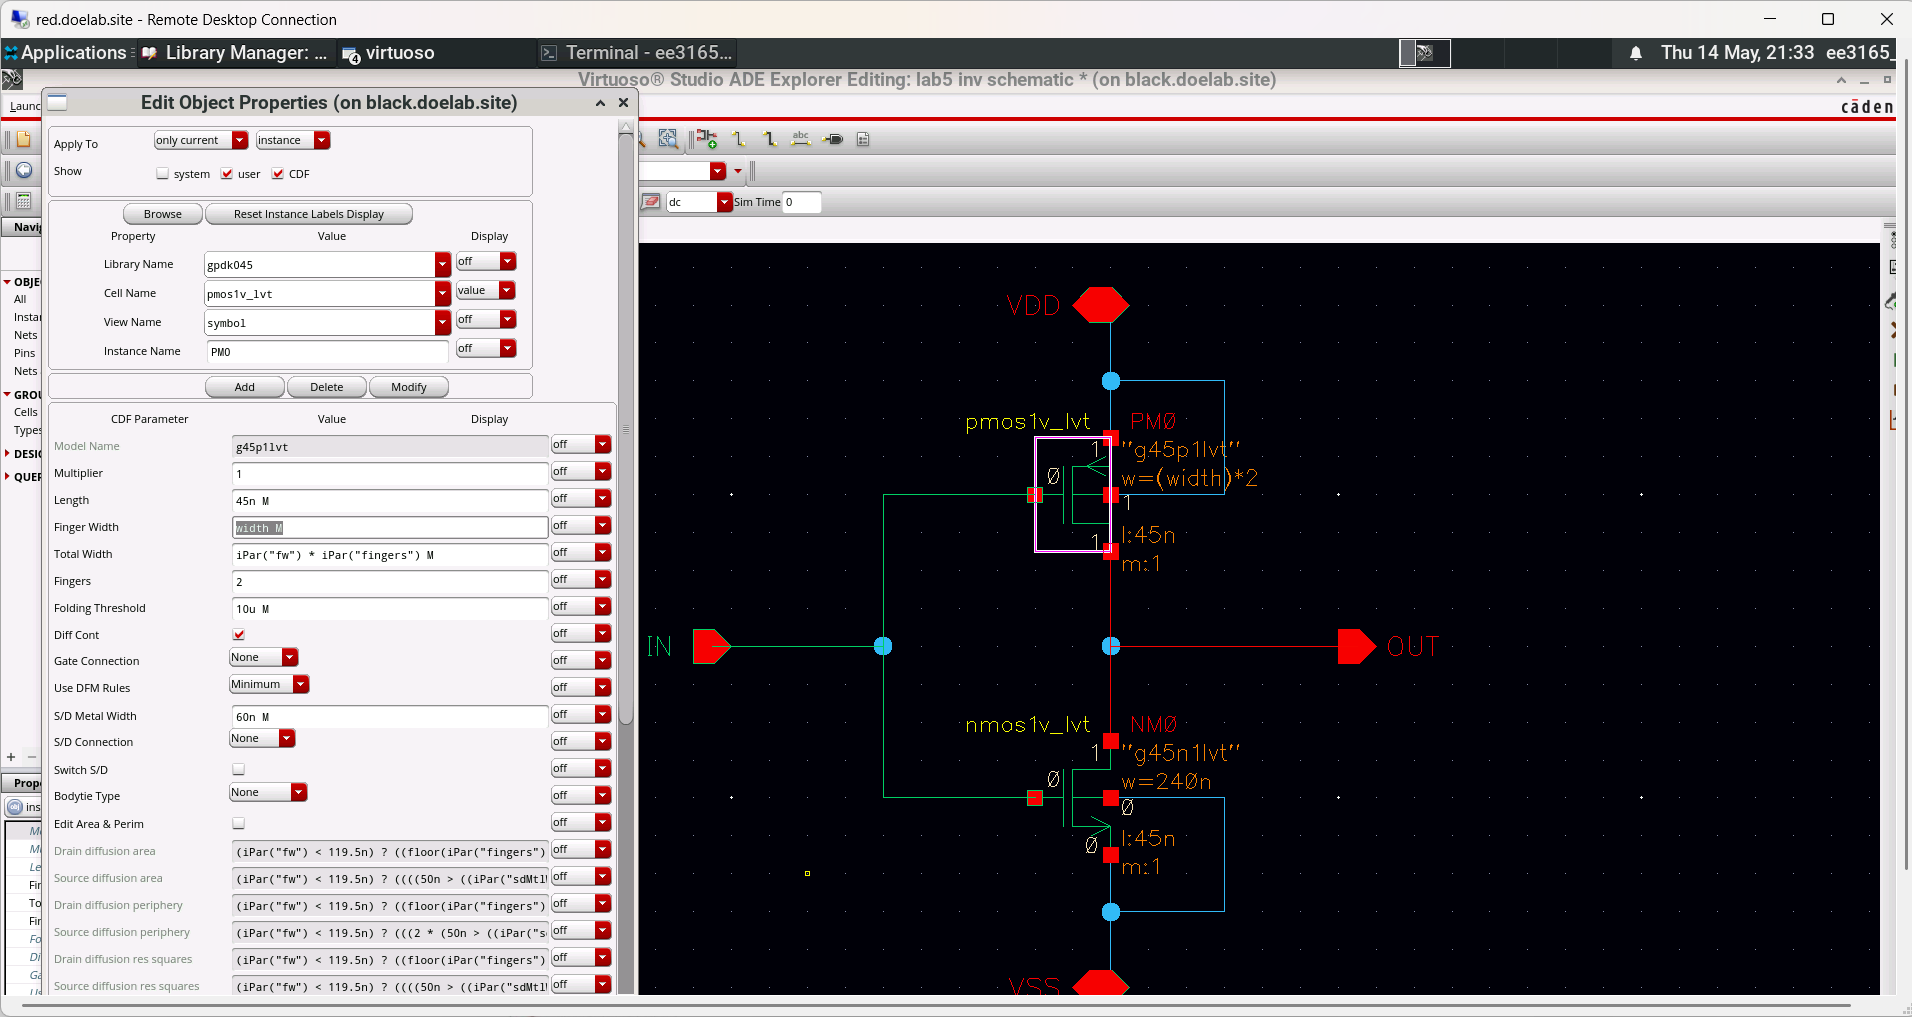
\includegraphics[width=0.7\textwidth]{inv_adjust_sizing.png}
    \caption{Hiệu chỉnh kích thước Finger Width của PMOS}
\end{figure}
\begin{figure}[H]
    \centering
    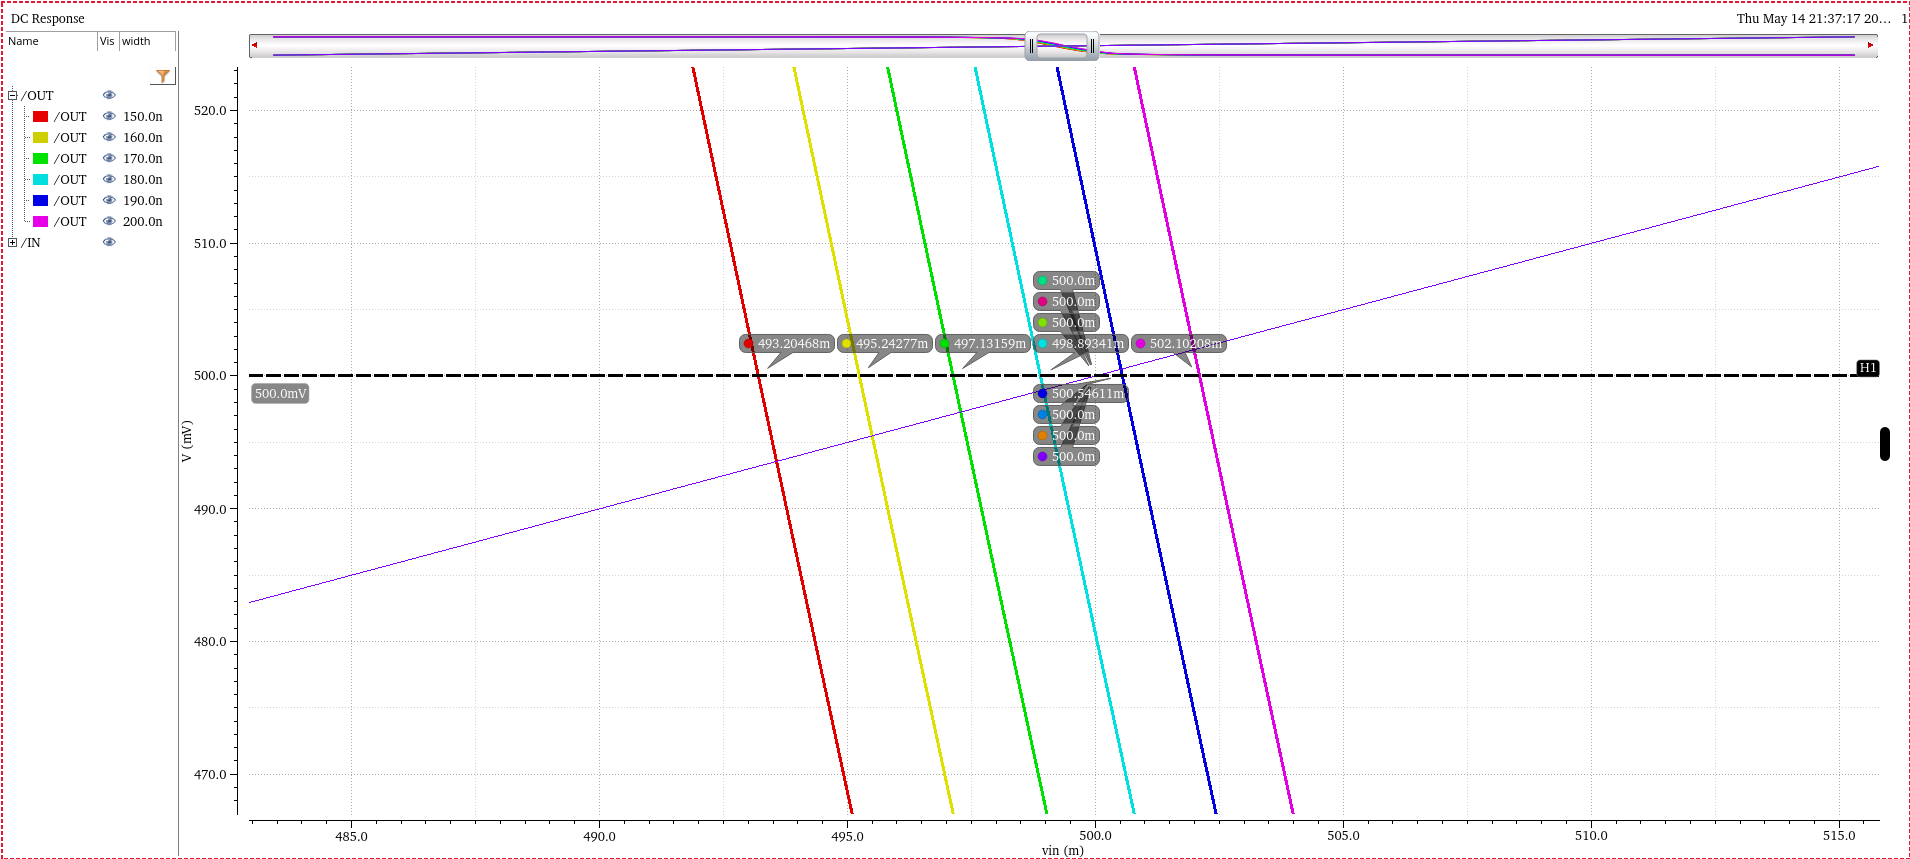
\includegraphics[width=0.7\textwidth]{inv_vm_sweep.png}
    \caption{Kết quả quét giá trị $V_M$ sau khi hiệu chỉnh (ví dụ tại $W=190ns$)}
\end{figure}

% =================================================================
% EXPERIMENT 2: NAND & NOR GATES
% =================================================================
\newpage
\section{Experiment 2: Circuit Design for CMOS NOR and NAND Gates}

\subsection{Cổng NAND}
\begin{itemize}
    \item \textbf{Bảng chân trị và Hoạt động:} (Trình bày bảng chân trị 2 ngõ vào).
    \item \textbf{Schematic và Symbol:}
    \begin{figure}[H]
        \centering
        \subfigure[Schematic NAND]{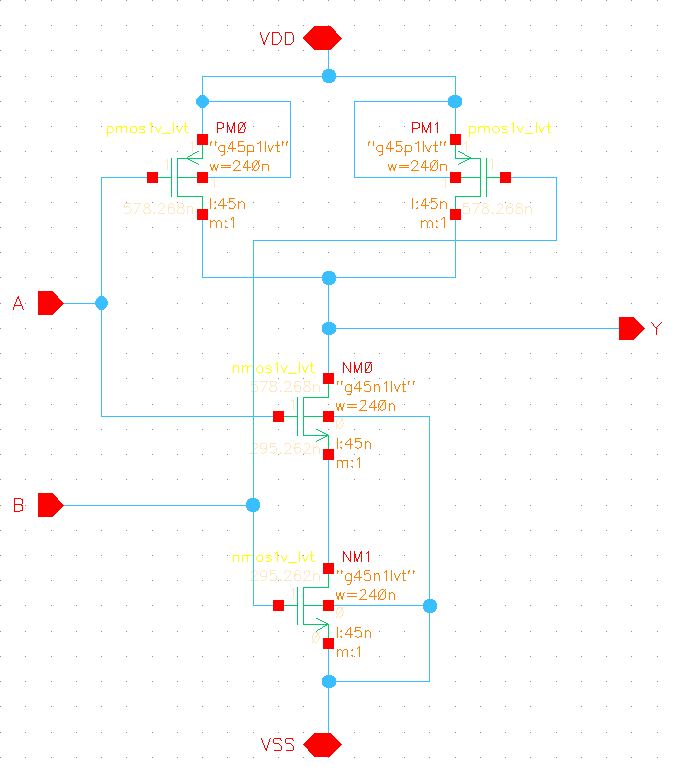
\includegraphics[width=0.45\textwidth]{nand_schematic.png}}
        \subfigure[Symbol NAND]{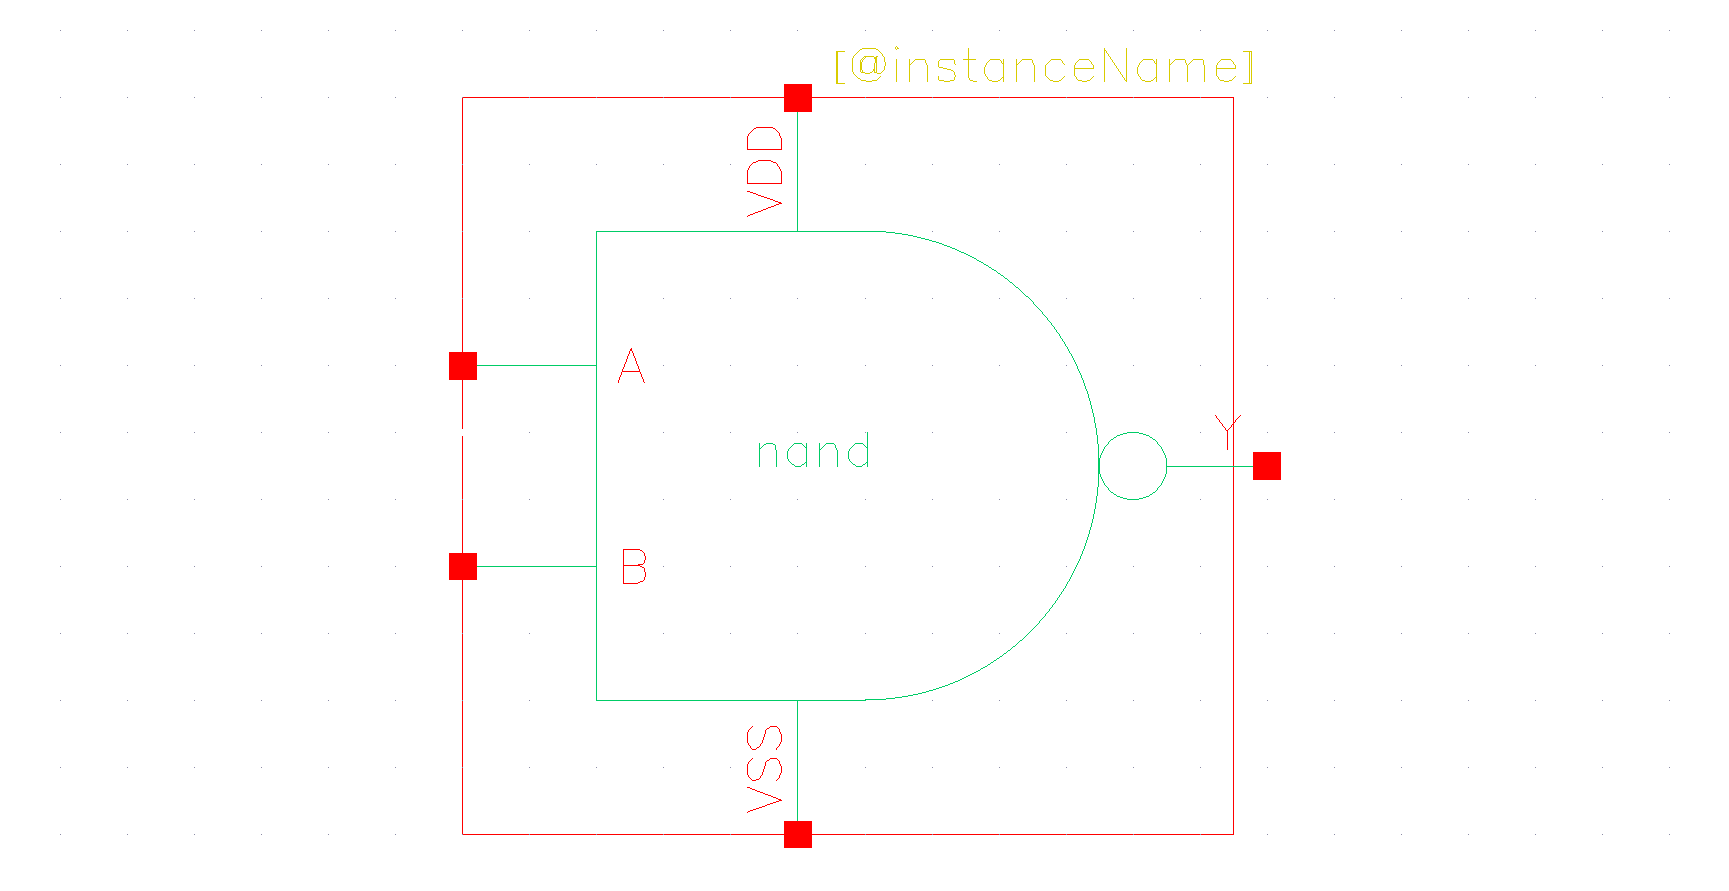
\includegraphics[width=0.45\textwidth]{nand_symbol.png}}
        \caption{Sơ đồ nguyên lý và Symbol cổng NAND}
    \end{figure}
    
    \item \textbf{Khảo sát DC (2 trường hợp):}
        \begin{enumerate}
            \item TH1: Thay đổi A, giữ B = 1.
            \item TH2: Thay đổi B, giữ A = 1.
        \end{enumerate}
    \begin{figure}[H]
        \centering
        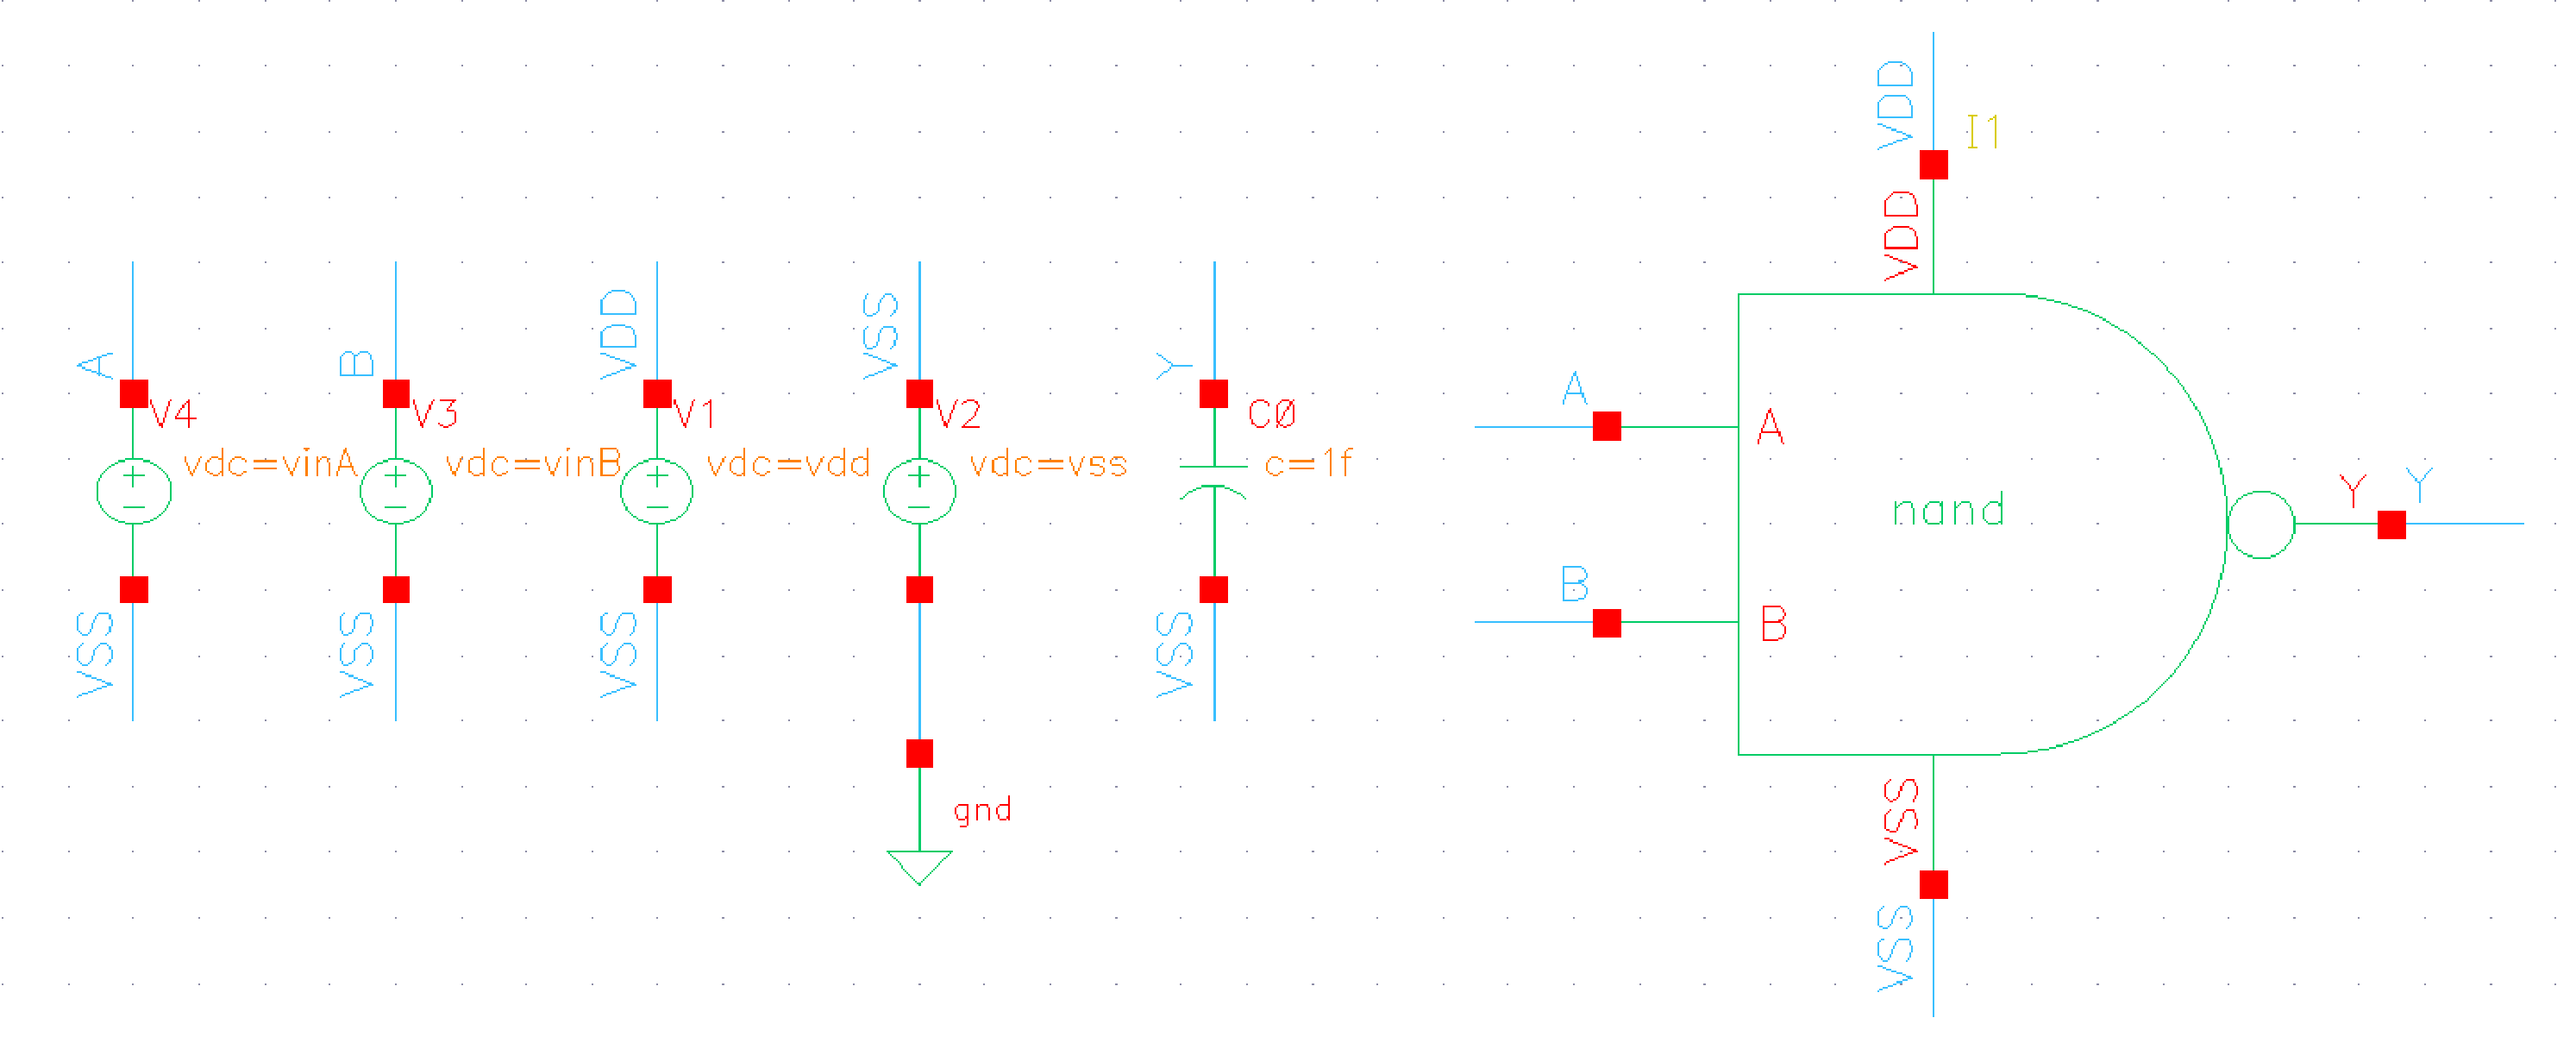
\includegraphics[width=0.7\textwidth]{nand_dc_testbench.png}
        \caption{Testbench DC cho cổng NAND}
    \end{figure}
    \begin{figure}[H]
        \centering
        \subfigure[DC Sweep A (B=1)]{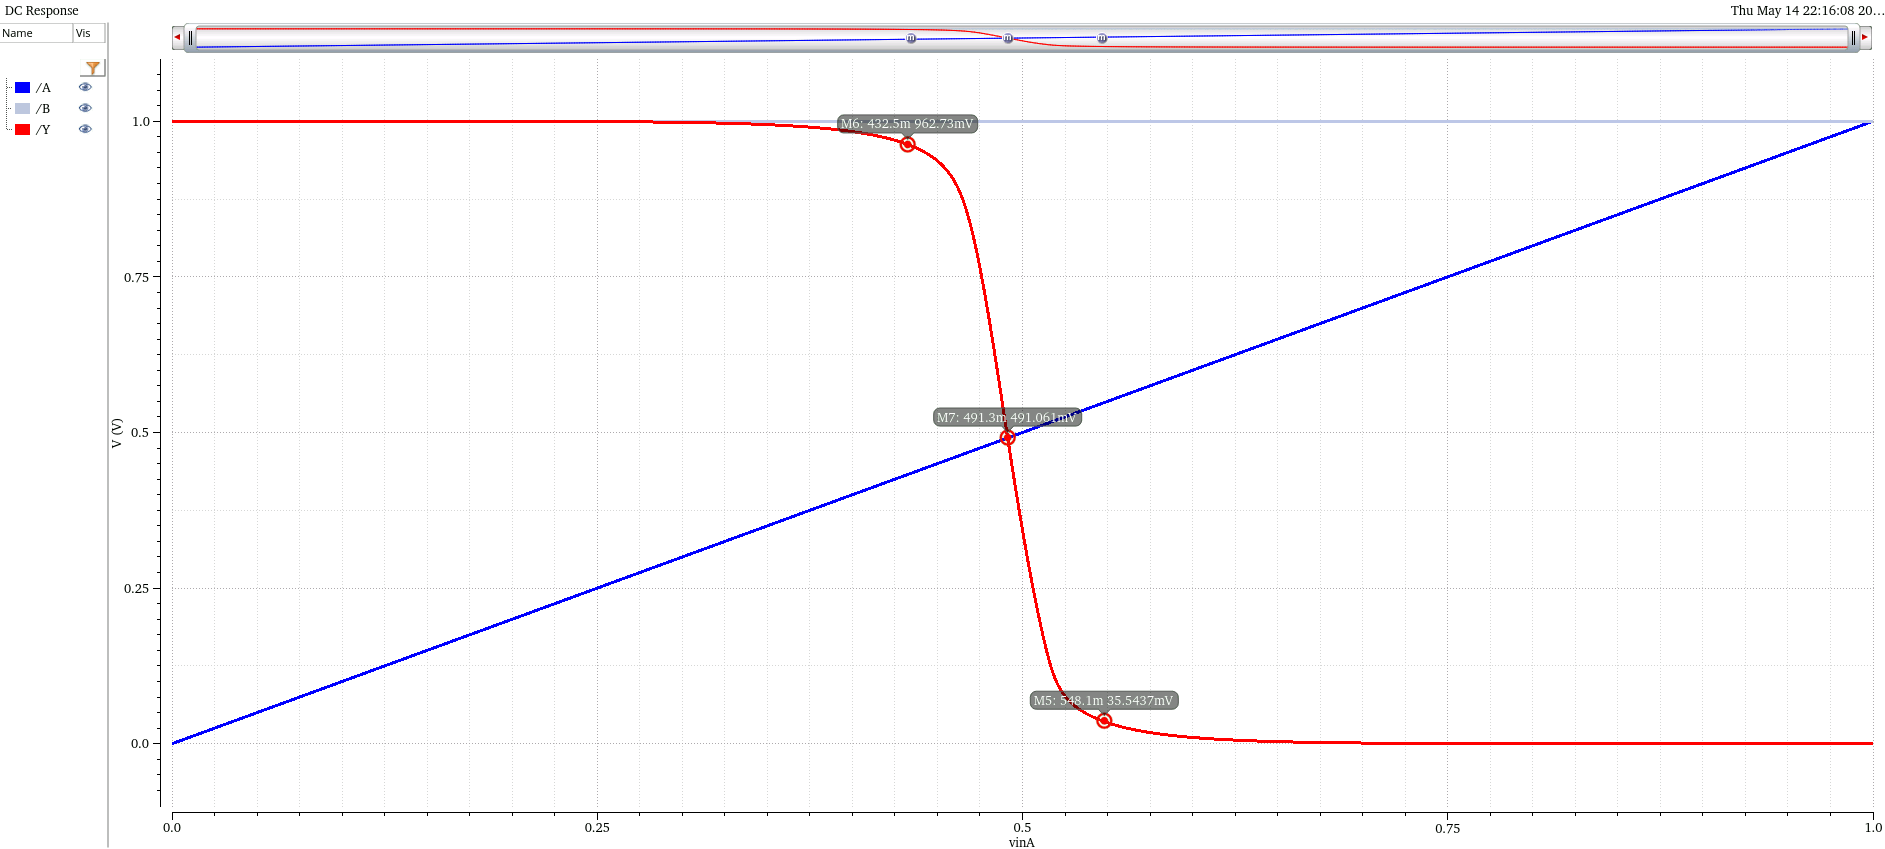
\includegraphics[width=0.45\textwidth]{nand_dc_sweep_A.png}}
        \subfigure[DC Sweep B (A=1)]{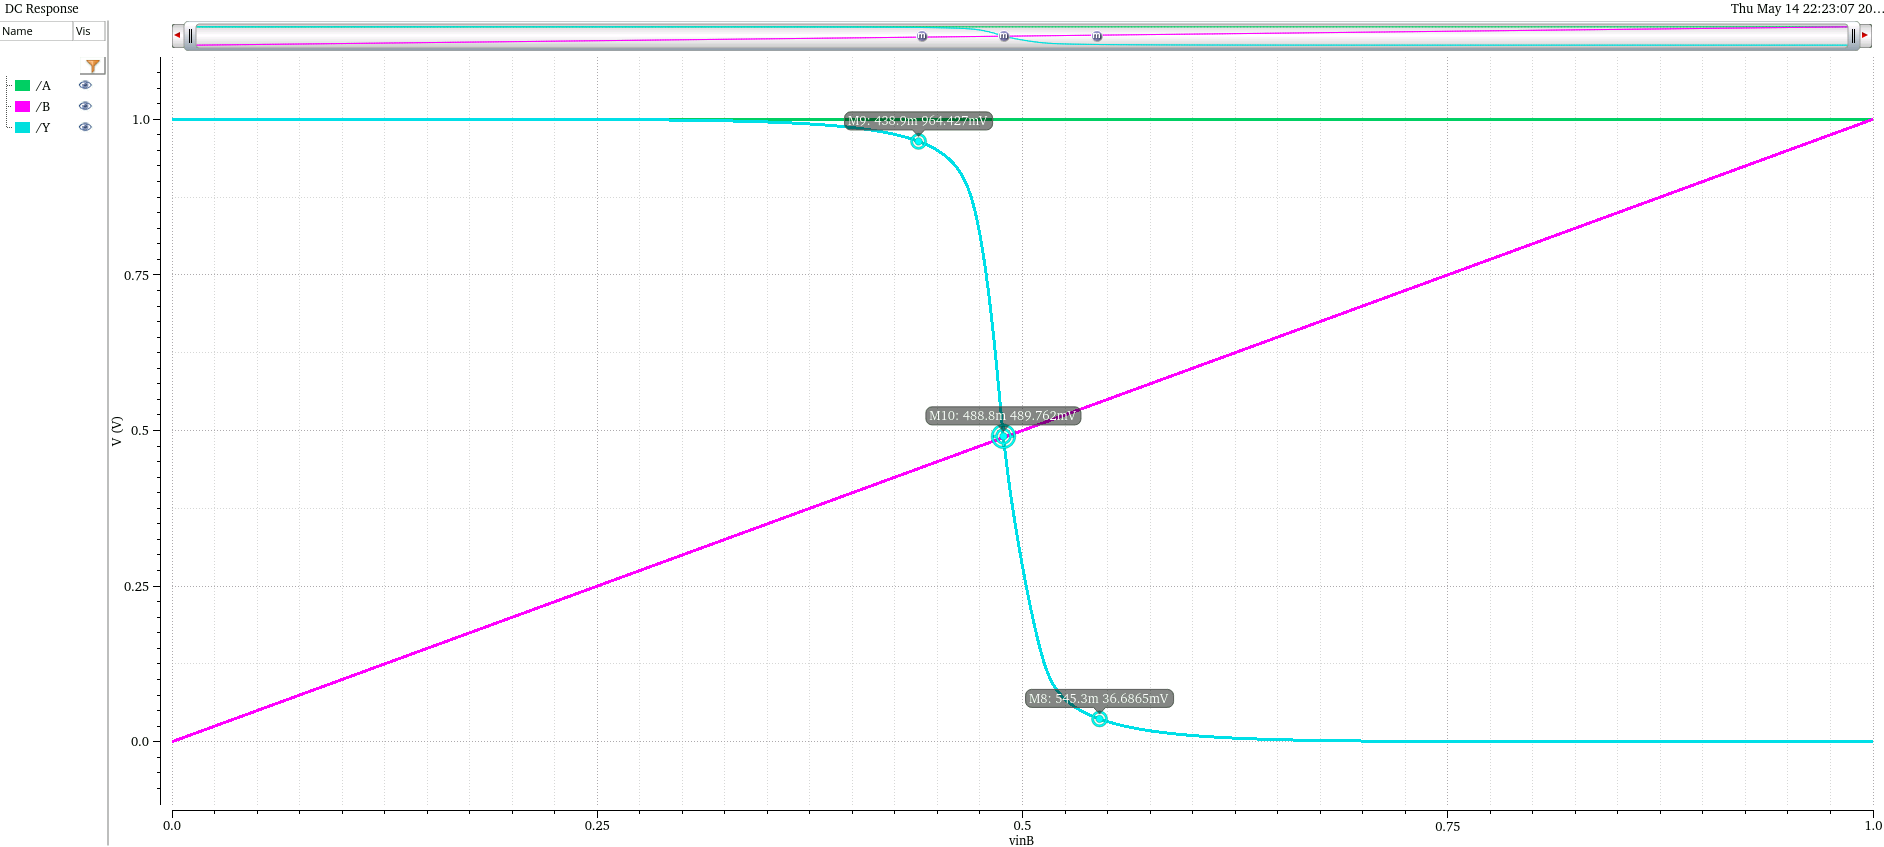
\includegraphics[width=0.45\textwidth]{nand_dc_sweep_B.png}}
        \caption{Đặc tuyến VTC của cổng NAND trong 2 trường hợp}
    \end{figure}

\textbf{Bảng giá trị ngõ ra theo ngõ vào cho TH1 (Step 0.1V):}
\begin{center}
    \begin{tabular}{|c|c|c|c|c|c|c|c|c|c|c|}
    \hline
    $V_{in}$ (V) & 0.1 & 0.2 & 0.3 & 0.4 & 0.5 & 0.6 & 0.7 & 0.8 & 0.9 & 1.0 \\ \hline
    $V_{out}$ (V) & 0.99 & 0.99 & 0.99 & 0.98 & 0.28 & 0.01 & 0.001 & 0.0001 & 0.00006 & 0.0000006 \\ \hline
    \end{tabular}
\end{center}

\textbf{Bảng giá trị ngõ ra theo ngõ vào cho TH2 (Step 0.1V):}
\begin{center}
    \begin{tabular}{|c|c|c|c|c|c|c|c|c|c|c|}
    \hline
    $V_{in}$ (V) & 0.1 & 0.2 & 0.3 & 0.4 & 0.5 & 0.6 & 0.7 & 0.8 & 0.9 & 1.0 \\ \hline
    $V_{out}$ (V) & 0.99 & 0.99 & 0.99 & 0.98 & 0.33 & 0.01 & 0.001 & 0.0001 & 0.00006 & 0.0000006 \\ \hline
    \end{tabular}
\end{center}

    \begin{table}[H]
        \centering
        \caption{Các thông số đặc tính tĩnh DC của cổng NAND 2 ngõ vào}
        \begin{tabular}{|c|c|c|c|c|c|c|}
        \hline
        \textbf{Case} & \textbf{State} & \textbf{$V_{IL}$ (V)} & \textbf{$V_{IH}$ (V)} & \textbf{$V_M$ (V)} & \textbf{$V_{OL}$ (V)} & \textbf{$V_{OH}$ (V)} \\ \hline
        Case 1 & A sweep, B = 1 & 0.3847 & 0.5369 & 0.4578 & 0.0039 & 0.9998  \\ \hline
        Case 2 & B sweep, A = 1 & 0.4285 & 0.5843 & 0.4996 & 0.0039 & 0.9998 \\ \hline
        \end{tabular}
    \end{table}

    \noindent\textbf{Ghi chú và giải thích các trường hợp khảo sát:}
    \begin{itemize}
        \item \textbf{Case 1 (A sweep, B = 1):} Ngõ vào B được giữ cố định ở mức logic cao ($V_{DD} = 1V$), ngõ vào A quét tuyến tính từ 0V đến 1V. Trong trường hợp này, PMOS nối với ngõ vào B ngắt hoàn toàn và NMOS tương ứng dẫn mạnh. Cổng NAND hoạt động tương tự như một mạch nghịch lưu (Inverter) đối với ngõ vào A. Do hiện tượng xếp chồng (stacking effect) của các transistor NMOS nối tiếp, điện áp ngưỡng chuyển mạch $V_M$ dịch chuyển nhẹ.
        \item \textbf{Case 2 (B sweep, A = 1):} Ngõ vào A được giữ cố định ở mức logic cao (1V), ngõ vào B quét tuyến tính từ 0V đến 1V. Do vị trí hình học của transistor NMOS nhận tín hiệu B nằm ở phía dưới (gần cực Ground hơn) so với NMOS nhận tín hiệu A, điện trở kênh dẫn hiệu dụng và hiệu ứng thân (body effect) có sự khác biệt. Điều này dẫn đến điện áp ngưỡng $V_M$ tăng lên đáng kể (0.4996V so với 0.4578V) và làm thay đổi lề nhiễu tĩnh ($NM_L, NM_H$).
    \end{itemize}

    \item \textbf{Mô phỏng Transient và Đo đạc thông số của trường hợp 1:}
    \begin{figure}[H]
        \centering
        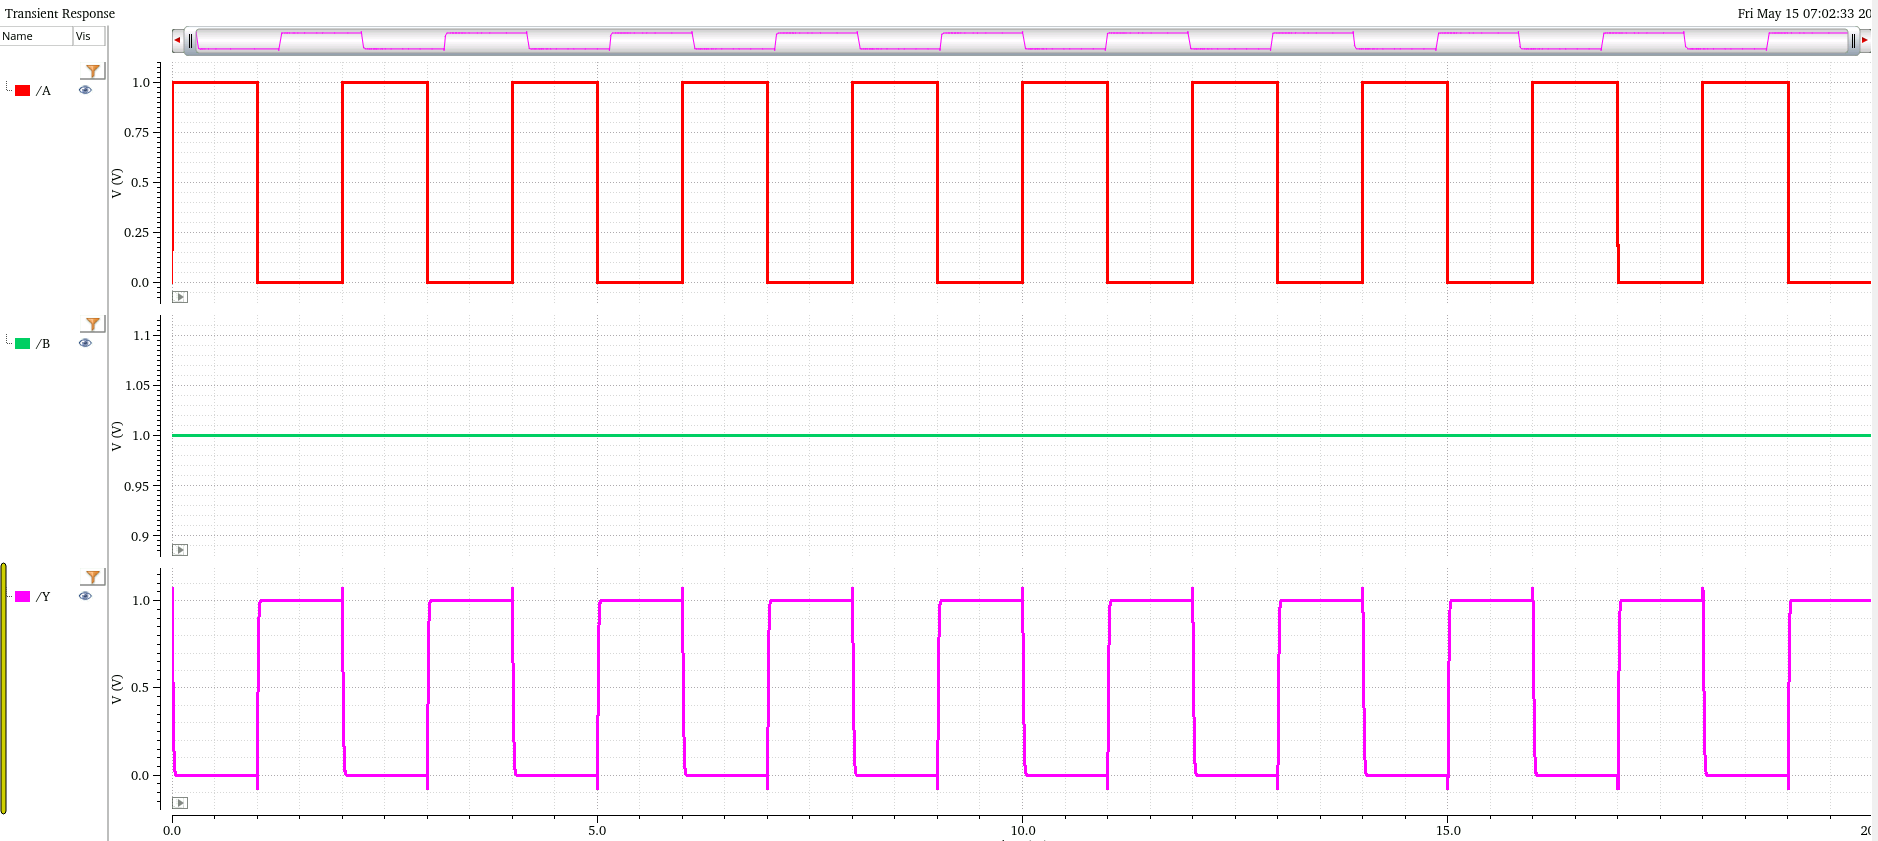
\includegraphics[width=0.8\textwidth]{nand_transient_waveforms.png}
        \caption{Kết quả mô phỏng Transient cổng NAND (Trường hợp 1)}
    \end{figure}

    % Bảng tổng hợp kết quả từ Calculator cho TH1
    \begin{table}[H]
        \centering
        \caption{Kết quả đo đạc thông số thời gian và công suất bằng Calculator (TH1)}
        \begin{tabular}{|c|c|c|c|c|c|c|c|}
        \hline
        \textbf{$t_{rise}$} & \textbf{$t_{fall}$} & \textbf{$t_{pdr}$} & \textbf{$t_{pdf}$} & \textbf{$t_{pd}$} & \textbf{Static Pwr 0} & \textbf{Static Pwr 1} & \textbf{Dynamic Pwr} \\ 
        \textbf{(ps)} & \textbf{(ps)} & \textbf{(ps)} & \textbf{(ps)} & \textbf{(ps)} & \textbf{(nW)} & \textbf{(nW)} & \textbf{($\mu$W)} \\ \hline
        17,71 & 21,75 & 10,65 & 12,58 & 11.195 & 14,5 & 13,2 & 0,746 \\ \hline
        \end{tabular}
    \end{table}

    \begin{figure}[H]
        \centering
        \subfigure[Đo $t_{rise}$]{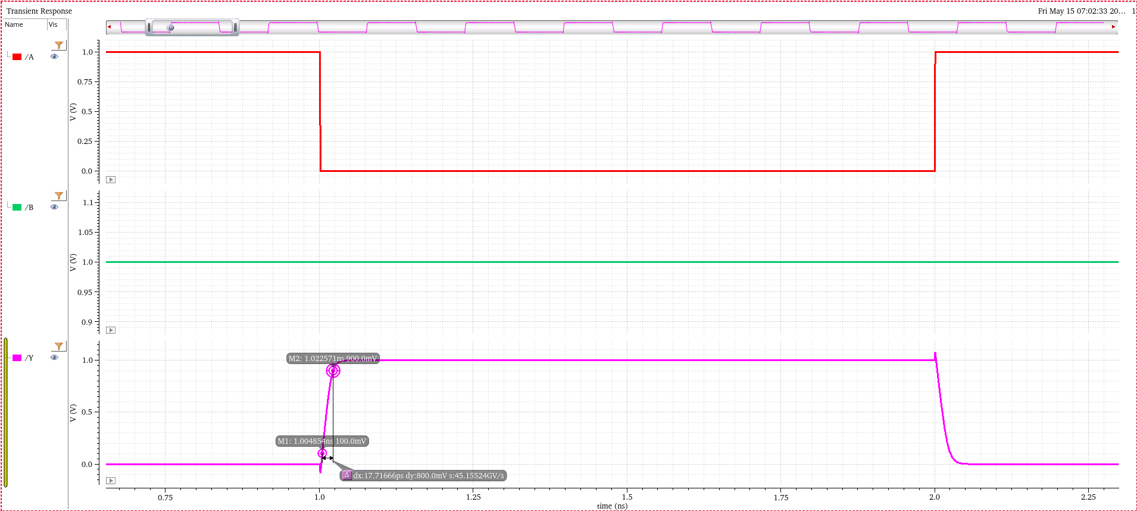
\includegraphics[width=0.5\textwidth]{nand_trise.png}}
        \subfigure[Calc $t_{rise}$]{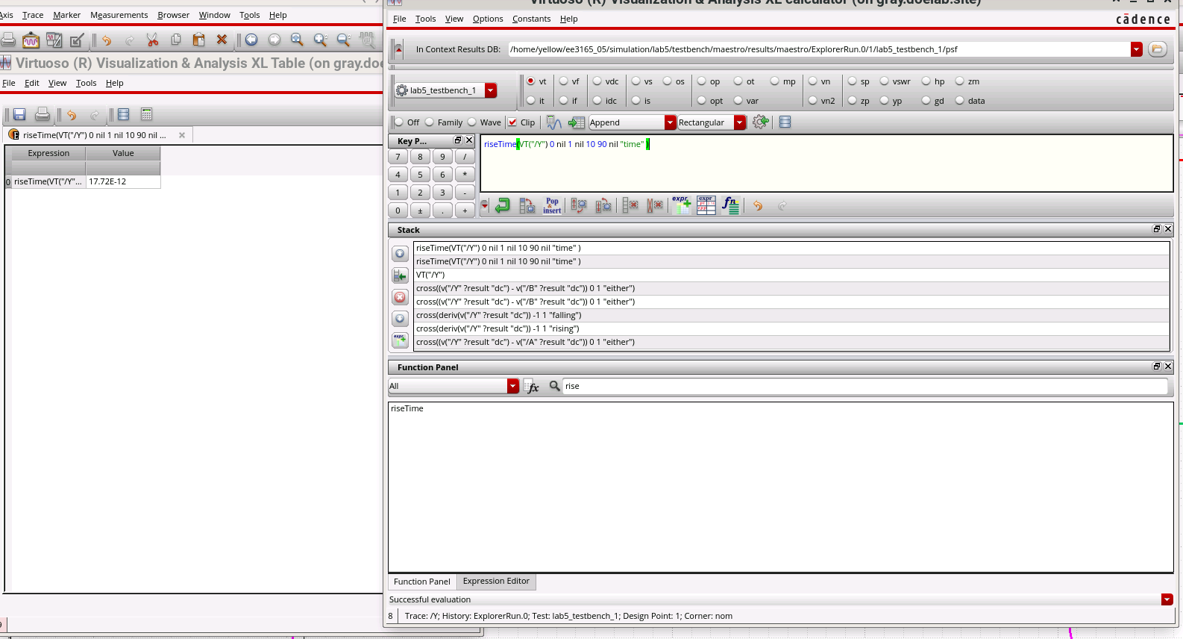
\includegraphics[width=0.5\textwidth]{nand_trise_calc.png}}
        \subfigure[Đo $t_{fall}$]{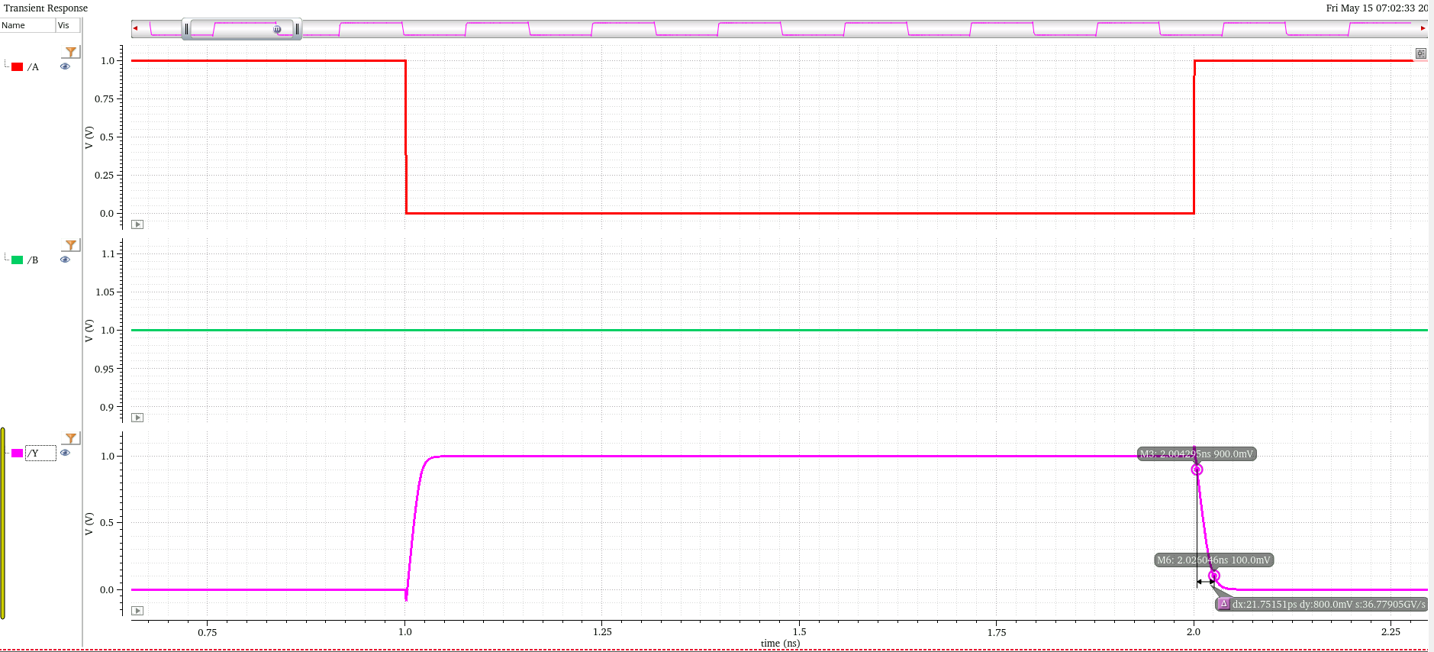
\includegraphics[width=0.5\textwidth]{nand_tfall.png}}
        \subfigure[Calc $t_{fall}$]{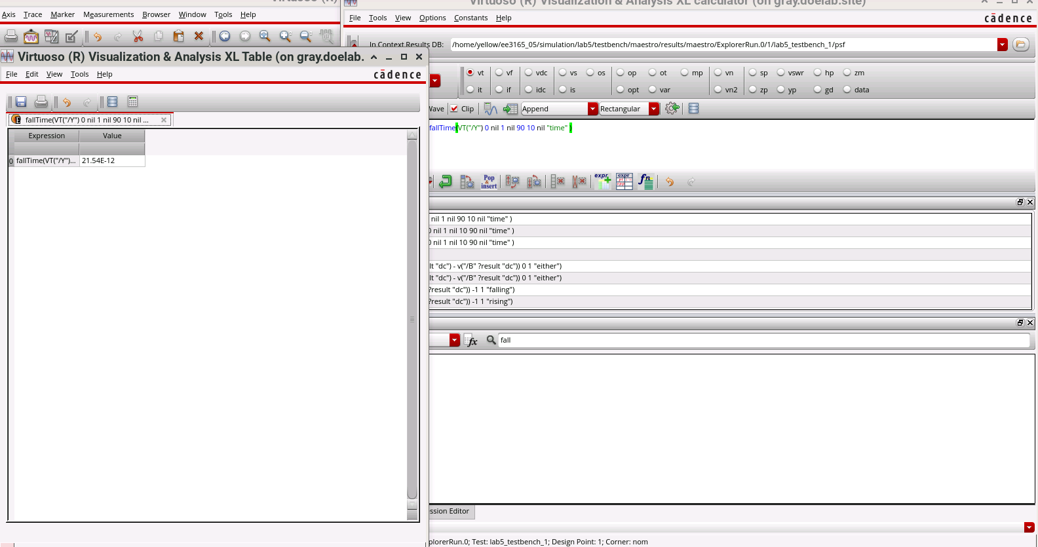
\includegraphics[width=0.5\textwidth]{nand_tfall_calc.png}}
        \caption{Thời gian cạnh lên và cạnh xuống cổng NAND kèm Calculator}
    \end{figure}
    \begin{figure}[H]
        \centering
        \subfigure[Đo $t_{pdr}$]{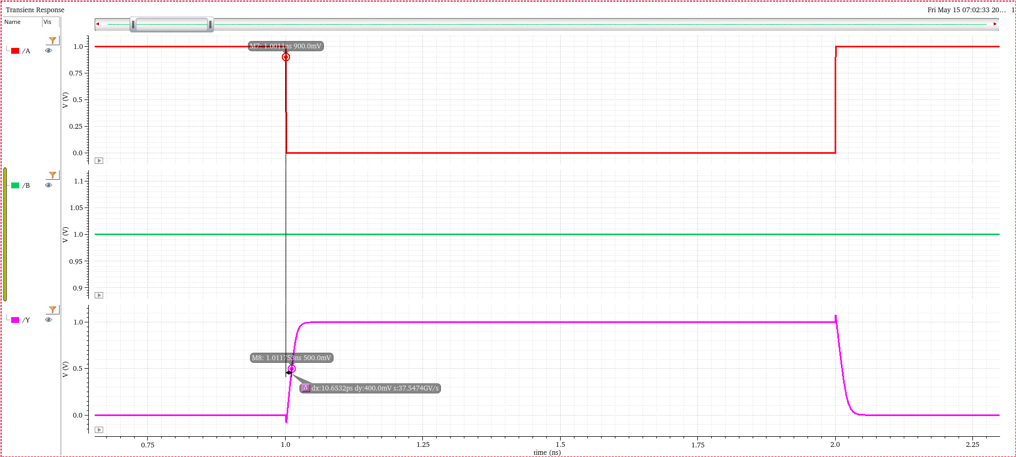
\includegraphics[width=0.5\textwidth]{nand_tpdr.png}}
        \subfigure[Calc $t_{pdr}$]{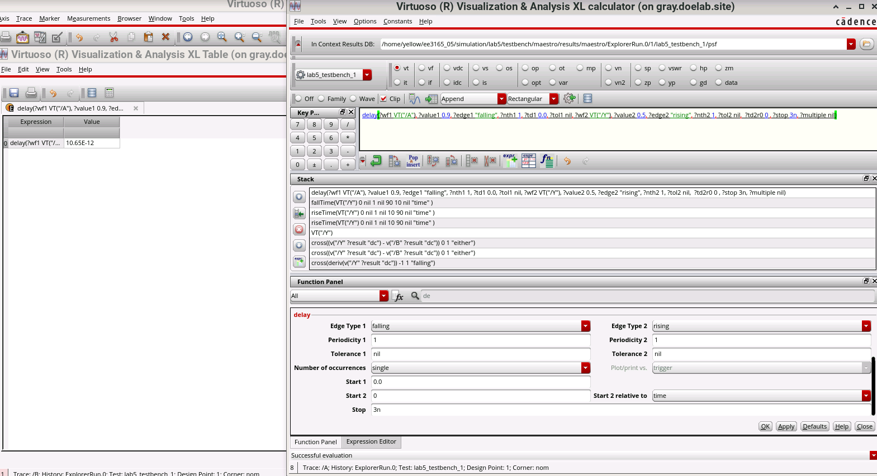
\includegraphics[width=0.5\textwidth]{nand_tpdr_calc.png}}
        \subfigure[Đo $t_{pdf}$]{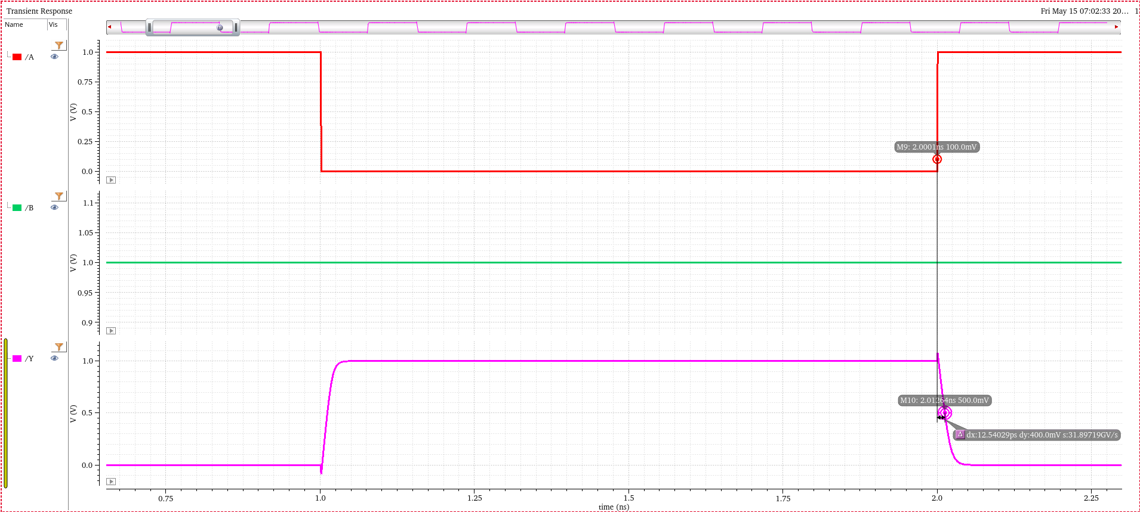
\includegraphics[width=0.5\textwidth]{nand_tpdf.png}}
        \subfigure[Calc $t_{pdf}$]{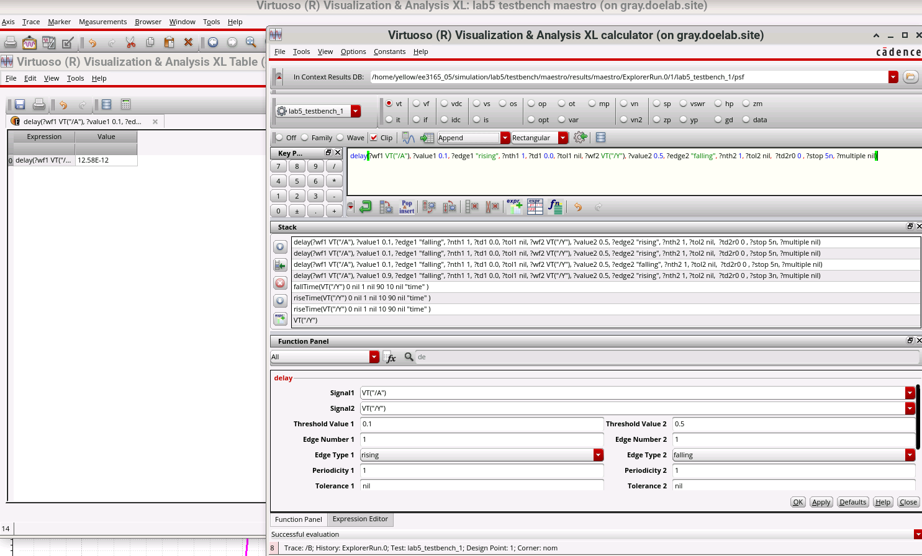
\includegraphics[width=0.5\textwidth]{nand_tpdf_calc.png}}
        \subfigure[Đo $t_{pd}$]{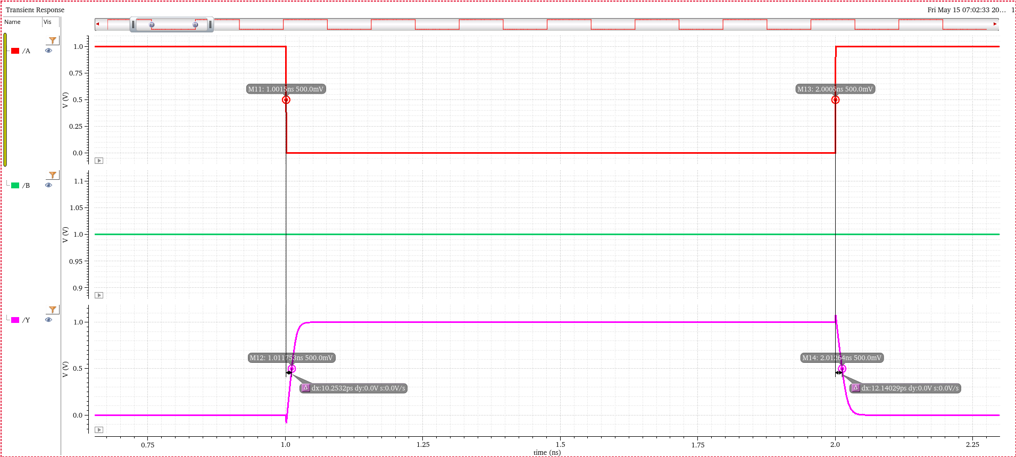
\includegraphics[width=0.5\textwidth]{nand_tpd.png}}
        \caption{Các thông số độ trễ cổng NAND kèm Calculator}
    \end{figure}
    \begin{figure}[H]
        \centering
        \subfigure[Static Pwr (0)]{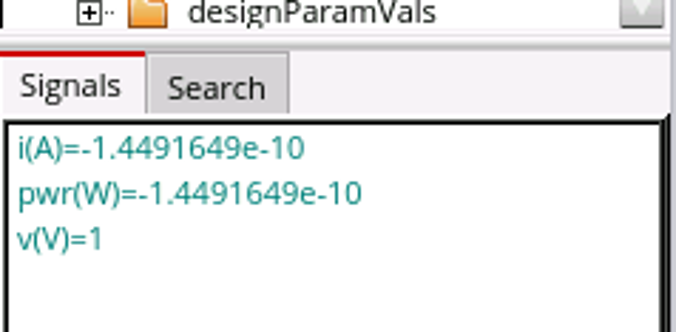
\includegraphics[width=0.6\textwidth]{nand_static_pwr_0.png}}
        \subfigure[Static Pwr (1)]{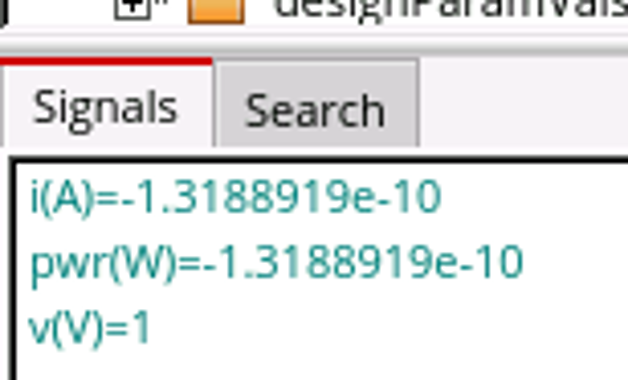
\includegraphics[width=0.6\textwidth]{nand_static_pwr_1.png}}
        \subfigure[Dynamic Pwr]{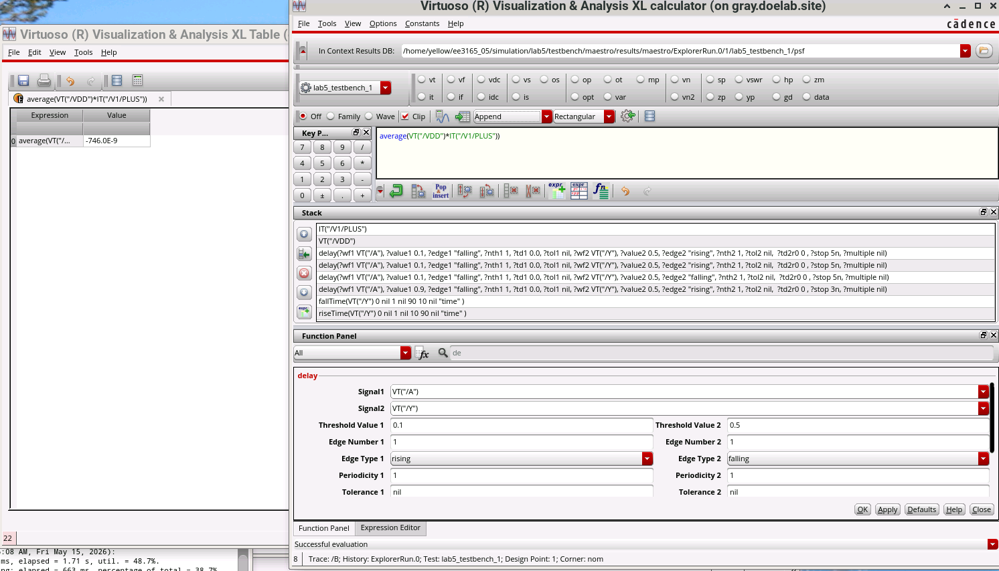
\includegraphics[width=0.6\textwidth]{nand_dynamic_pwr.png}}
        \caption{Công suất tĩnh và động cổng NAND}
    \end{figure}

    \item \textbf{Mô phỏng Transient và Đo đạc thông số của trường hợp 2:}
    \begin{figure}[H]
        \centering
        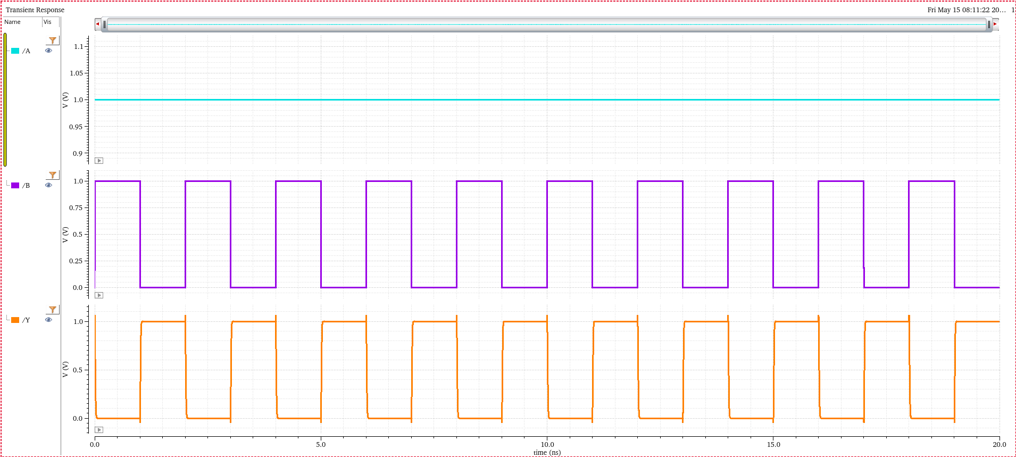
\includegraphics[width=0.8\textwidth]{nand2_transient_waveforms.png}
        \caption{Kết quả mô phỏng Transient cổng NAND}
    \end{figure}
% Bảng tổng hợp kết quả từ Calculator cho TH2
    \begin{table}[H]
        \centering
        \caption{Kết quả đo đạc thông số thời gian và công suất bằng Calculator (TH2)}
        \begin{tabular}{|c|c|c|c|c|c|c|c|}
        \hline
        \textbf{$t_{rise}$} & \textbf{$t_{fall}$} & \textbf{$t_{pdr}$} & \textbf{$t_{pdf}$} & \textbf{$t_{pd}$} & \textbf{Static Pwr 0} & \textbf{Static Pwr 1} & \textbf{Dynamic Pwr} \\ 
        \textbf{(ps)} & \textbf{(ps)} & \textbf{(ps)} & \textbf{(ps)} & \textbf{(ps)} & \textbf{(nW)} & \textbf{(nW)} & \textbf{(nW)} \\ \hline
        20,38 & 21,8 & 12,68 & 14,21 & 13,05 & 13,7 & 13,2 & 19,14 \\ \hline
        \end{tabular}
    \end{table}

    \begin{figure}[H]
        \centering
        \subfigure[Đo $t_{rise}$]{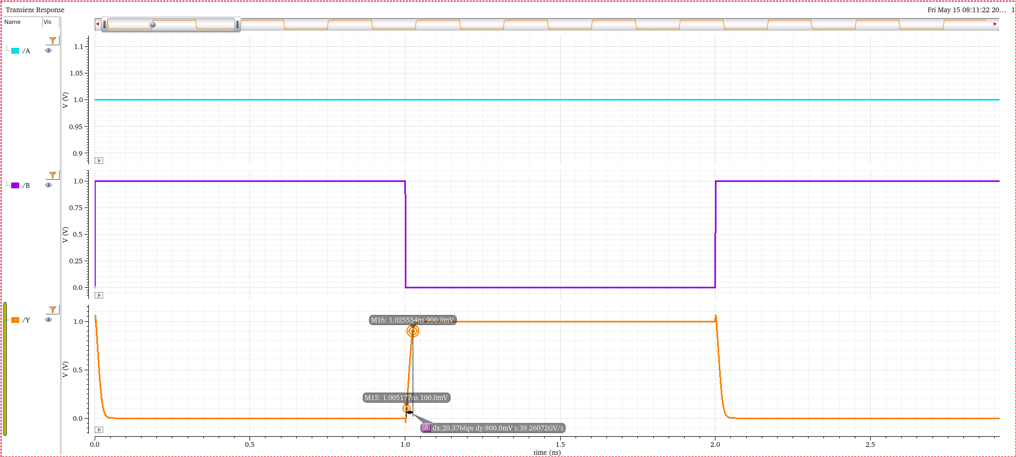
\includegraphics[width=0.5\textwidth]{nand2_trise.png}}
        \subfigure[Calc $t_{rise}$]{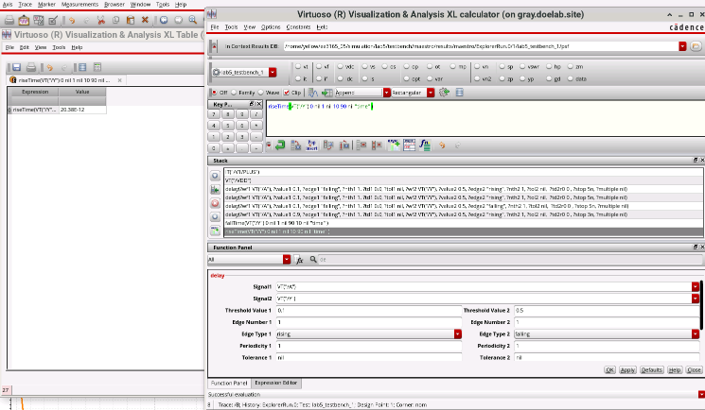
\includegraphics[width=0.5\textwidth]{nand2_trise_calc.png}}
        \subfigure[Đo $t_{fall}$]{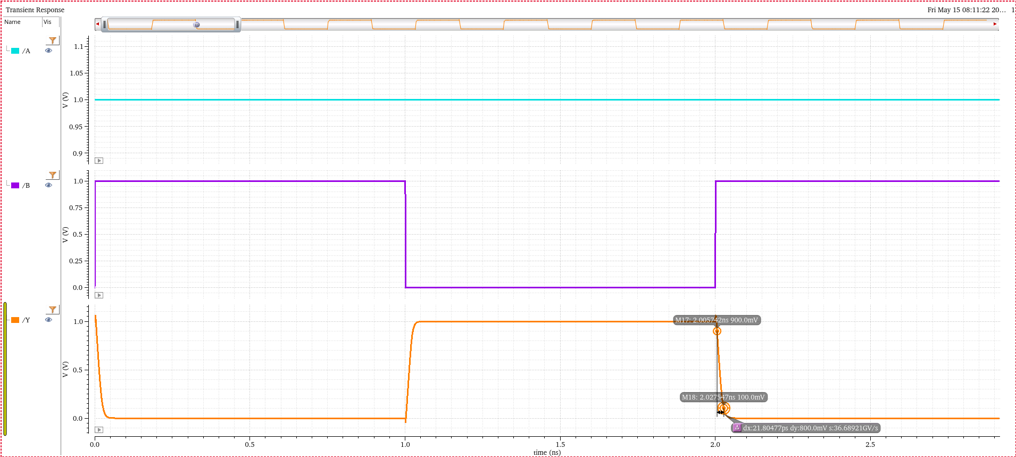
\includegraphics[width=0.5\textwidth]{nand2_tfall.png}}
        \subfigure[Calc $t_{fall}$]{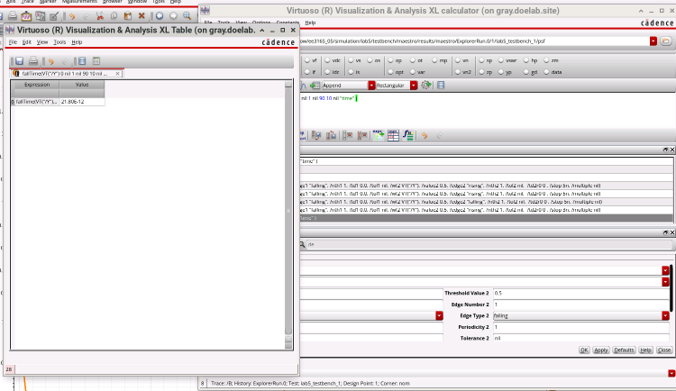
\includegraphics[width=0.5\textwidth]{nand2_tfall_calc.png}}
        \caption{Thời gian cạnh lên và cạnh xuống cổng NAND kèm Calculator}
    \end{figure}
    \begin{figure}[H]
        \centering
        \subfigure[Đo $t_{pdr}$]{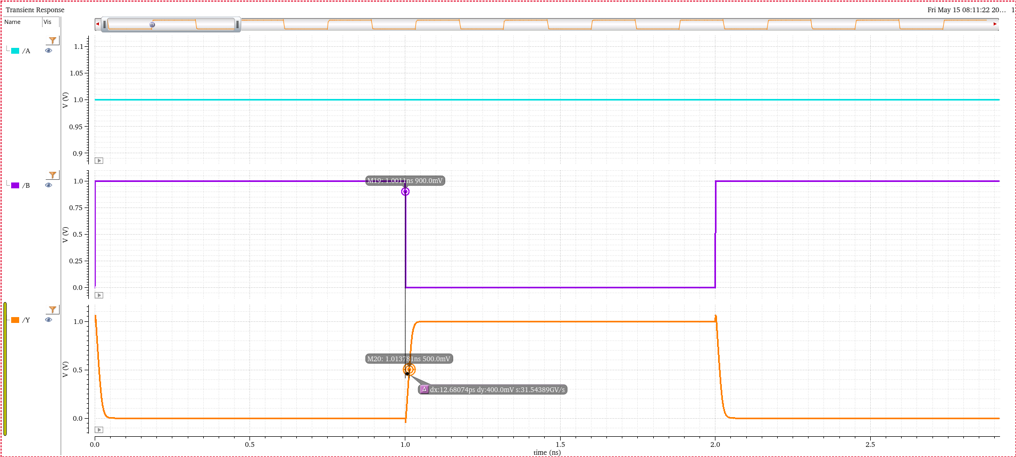
\includegraphics[width=0.5\textwidth]{nand2_tpdr.png}}
        \subfigure[Calc $t_{pdr}$]{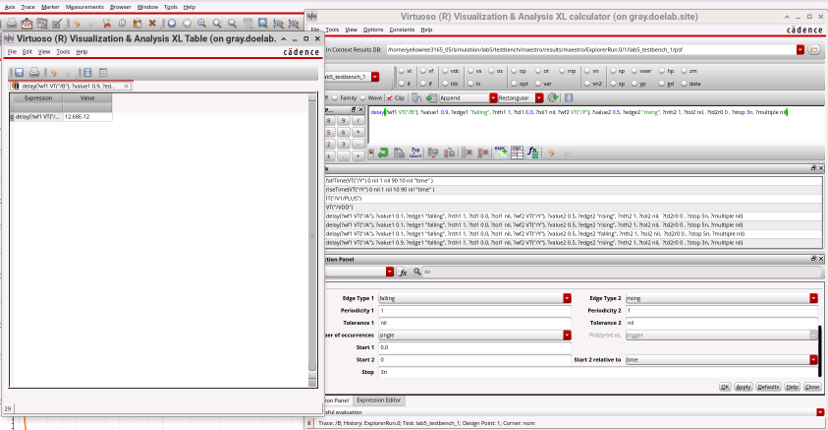
\includegraphics[width=0.5\textwidth]{nand2_tpdr_calc.png}}
        \subfigure[Đo $t_{pdf}$]{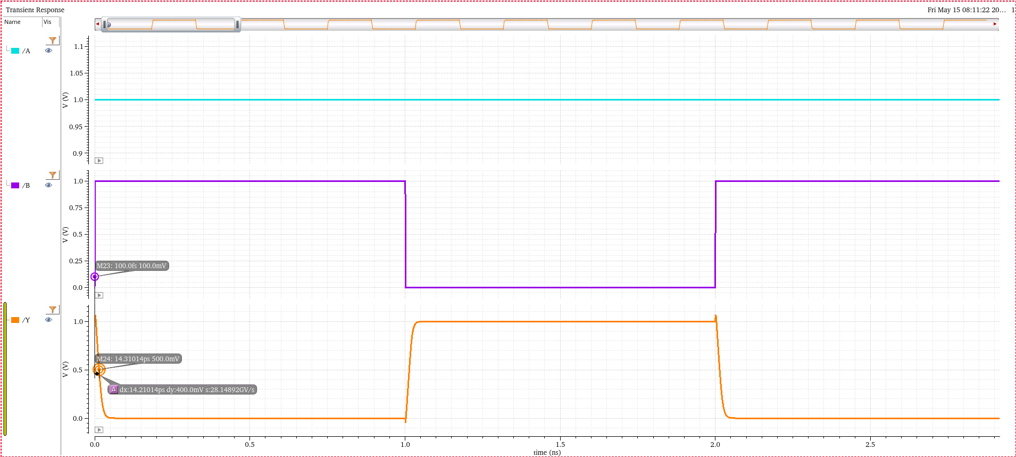
\includegraphics[width=0.5\textwidth]{nand2_tpdf.png}}
        \subfigure[Calc $t_{pdr}$]{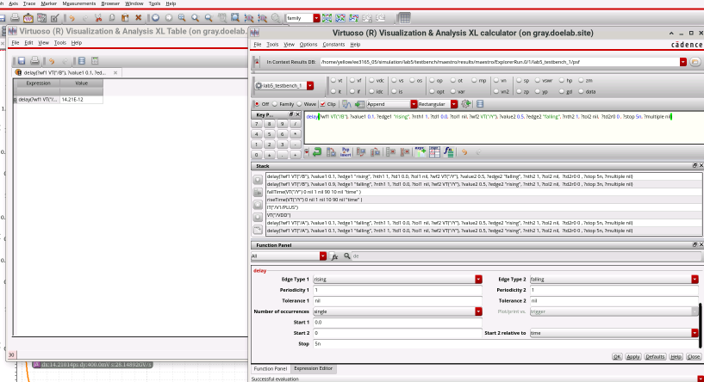
\includegraphics[width=0.5\textwidth]{nand2_tpdf_calc.png}}
        \subfigure[Đo $t_{pd}$]{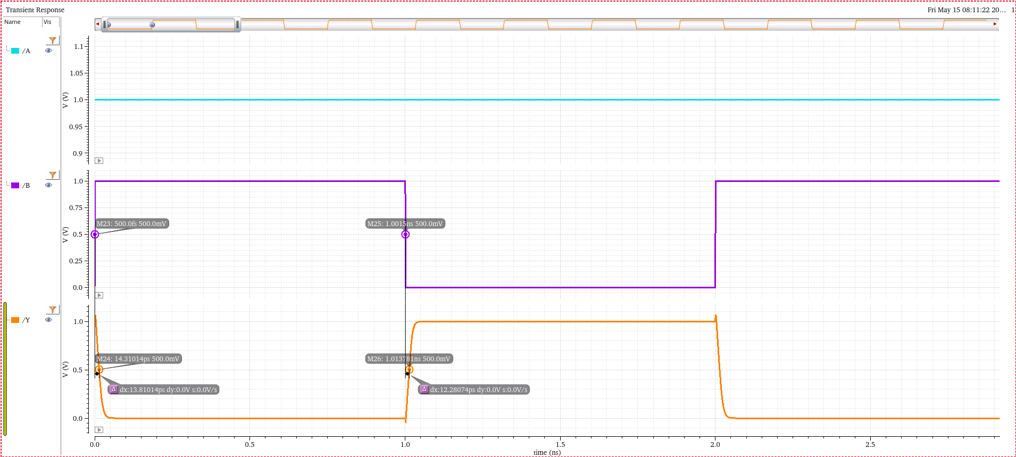
\includegraphics[width=0.5\textwidth]{nand2_tpd.png}}
        \caption{Các thông số độ trễ cổng NAND}
    \end{figure}
    \begin{figure}[H]
        \centering
        \subfigure[Static Pwr (0)]{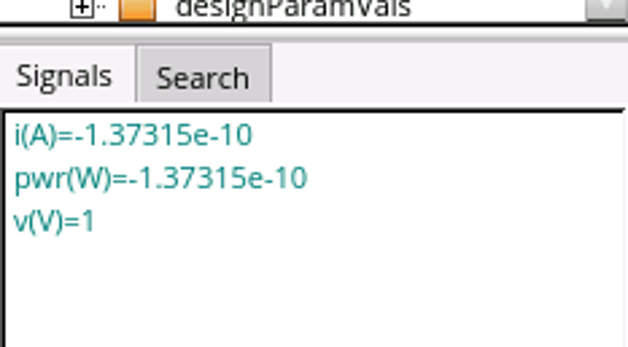
\includegraphics[width=0.5\textwidth]{nand2_static_pwr_0.png}}
        \subfigure[Static Pwr (1)]{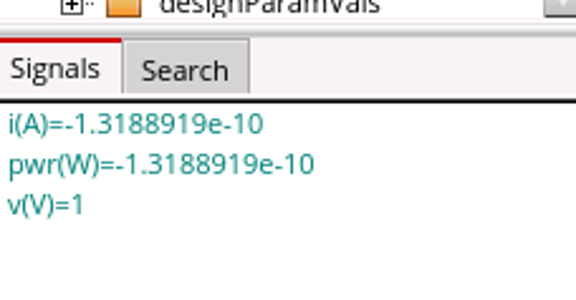
\includegraphics[width=0.5\textwidth]{nand2_static_pwr_1.png}}
        \subfigure[Dynamic Pwr]{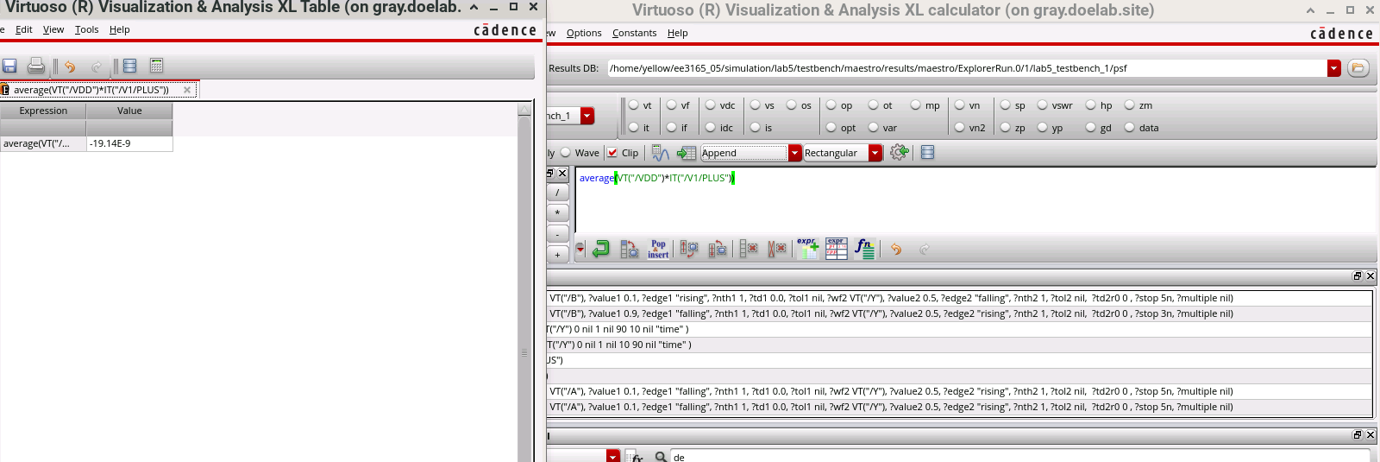
\includegraphics[width=0.5\textwidth]{nand2_dynamic_pwr.png}}
        \caption{Công suất tĩnh và động cổng NAND}
    \end{figure}

    \item \textbf{Hiệu chỉnh kích thước (Adjust $V_M = V_{DD}/2$):}

Để đạt được điện áp chuyển mạch $V_M \approx V_{DD}/2$, kích thước của transistor PMOS được tăng lên so với NMOS nhằm bù lại độ linh động hạt tải của PMOS thấp hơn so với NMOS. Bằng cách ta sẽ thay đổi giá trị Finger Width của cả 2 Pmos. Đầu tiên ta sẽ đặt biến width M vào chỗ Finger Width để quét giá trị.

    \begin{figure}[H]
        \centering
        \subfigure[Thiết lập Sweep]{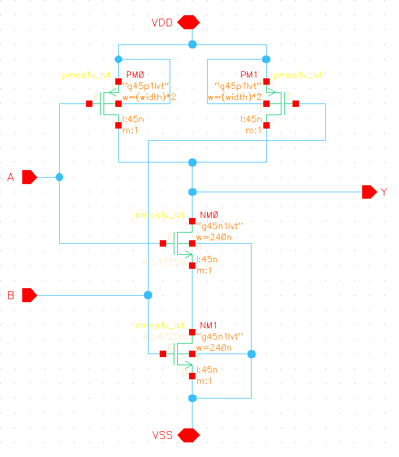
\includegraphics[width=0.5\textwidth]{nand_sizing_setup.png}}
        \subfigure[Kết quả Sweep VTC TH1 tại width=165ns]{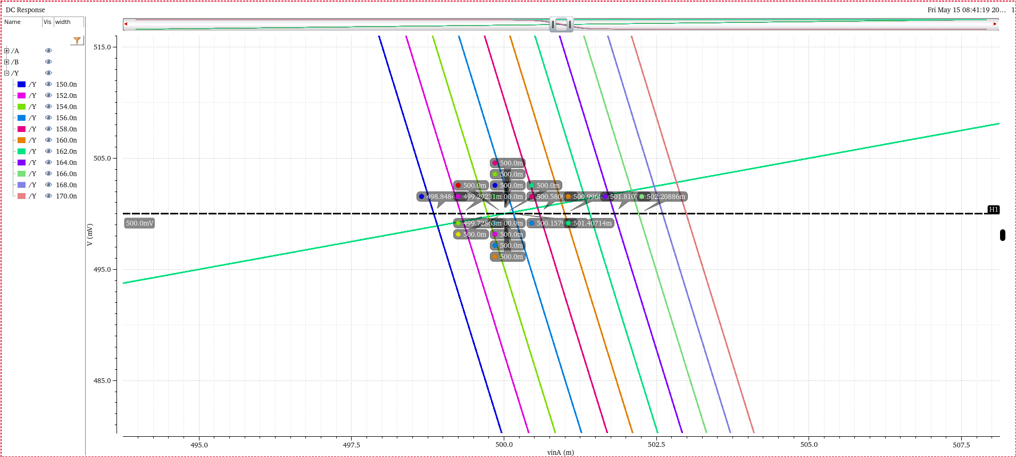
\includegraphics[width=0.65\textwidth]{nand_sizing_result1.png}}
        \subfigure[Kết quả Sweep VTC TH2 tại width=170ns]{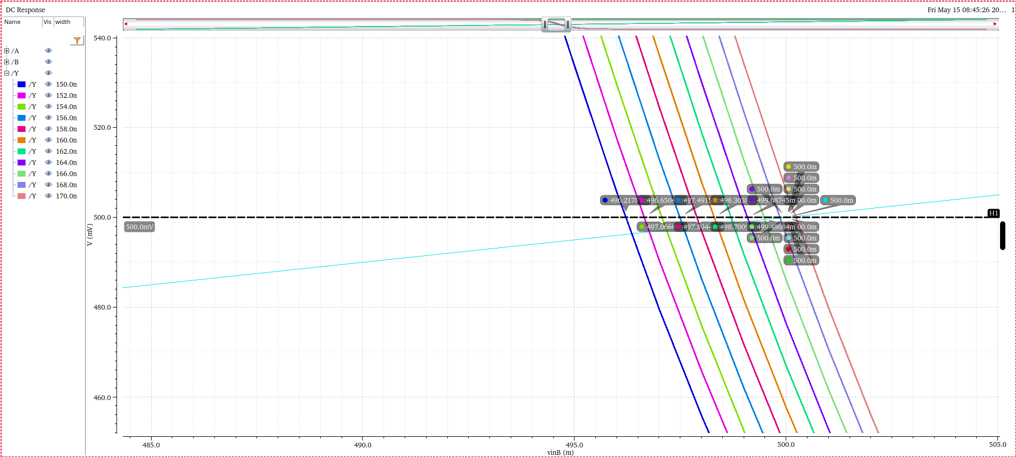
\includegraphics[width=0.65\textwidth]{nand_sizing_result2.png}}
        \caption{Hiệu chỉnh kích thước để tối ưu điểm chuyển mạch cho cổng NAND}
    \end{figure}
\end{itemize}

\subsection{Cổng NOR}
\begin{itemize}
    \item \textbf{Bảng chân trị và Hoạt động:} (Trình bày bảng chân trị).
    \item \textbf{Schematic và Symbol:}
    \begin{figure}[H]
        \centering
        \subfigure[Schematic NOR]{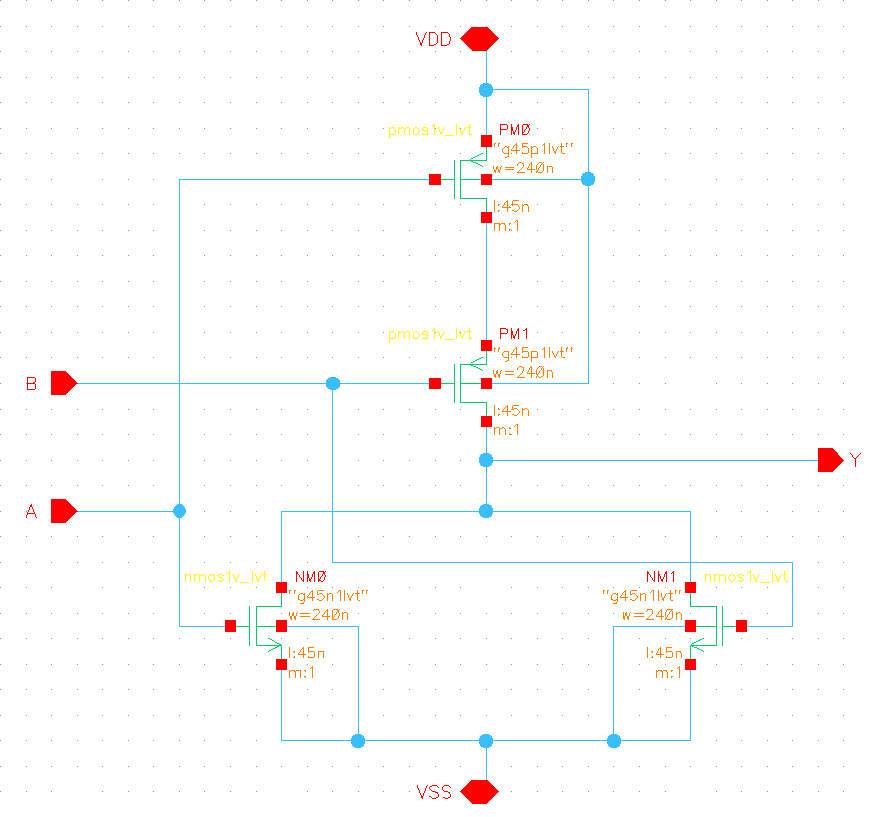
\includegraphics[width=0.45\textwidth]{nor_schematic.png}}
        \subfigure[Symbol NOR]{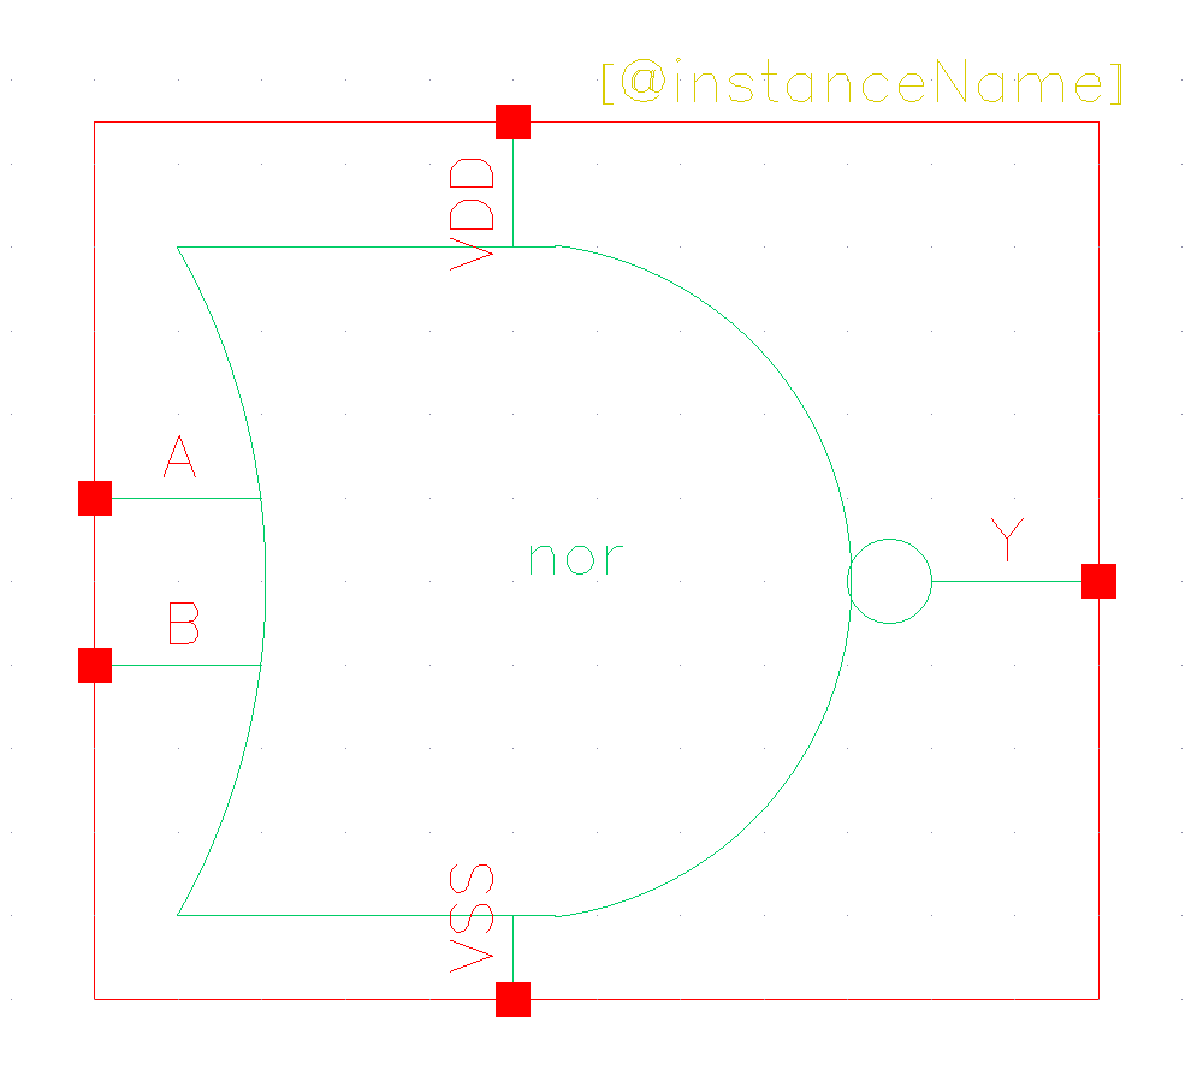
\includegraphics[width=0.45\textwidth]{nor_symbol.png}}
        \caption{Sơ đồ nguyên lý và Symbol cổng NOR}
    \end{figure}
    
    \item \textbf{Khảo sát DC (2 trường hợp):}
        \begin{enumerate}
            \item TH1: Thay đổi A, giữ B = 0.
            \item TH2: Thay đổi B, giữ A = 0.
        \end{enumerate}
    \begin{figure}[H]
        \centering
        \subfigure[DC Sweep A (B=0)]{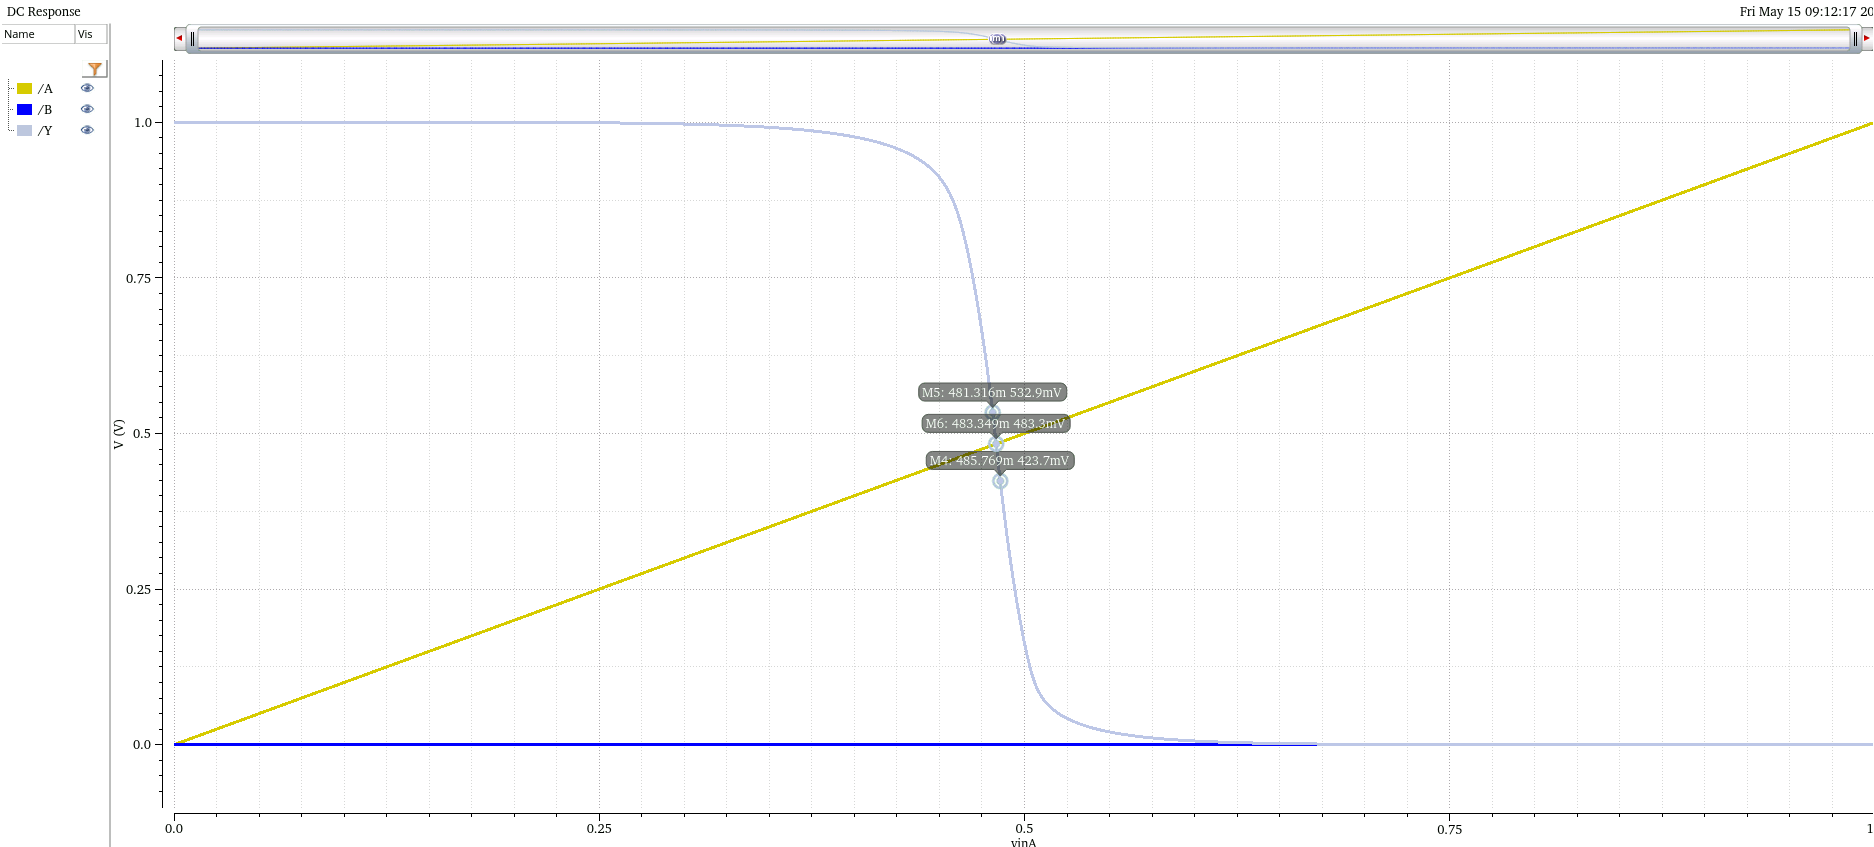
\includegraphics[width=0.45\textwidth]{nor_dc_sweep_A.png}}
        \subfigure[DC Sweep B (A=0)]{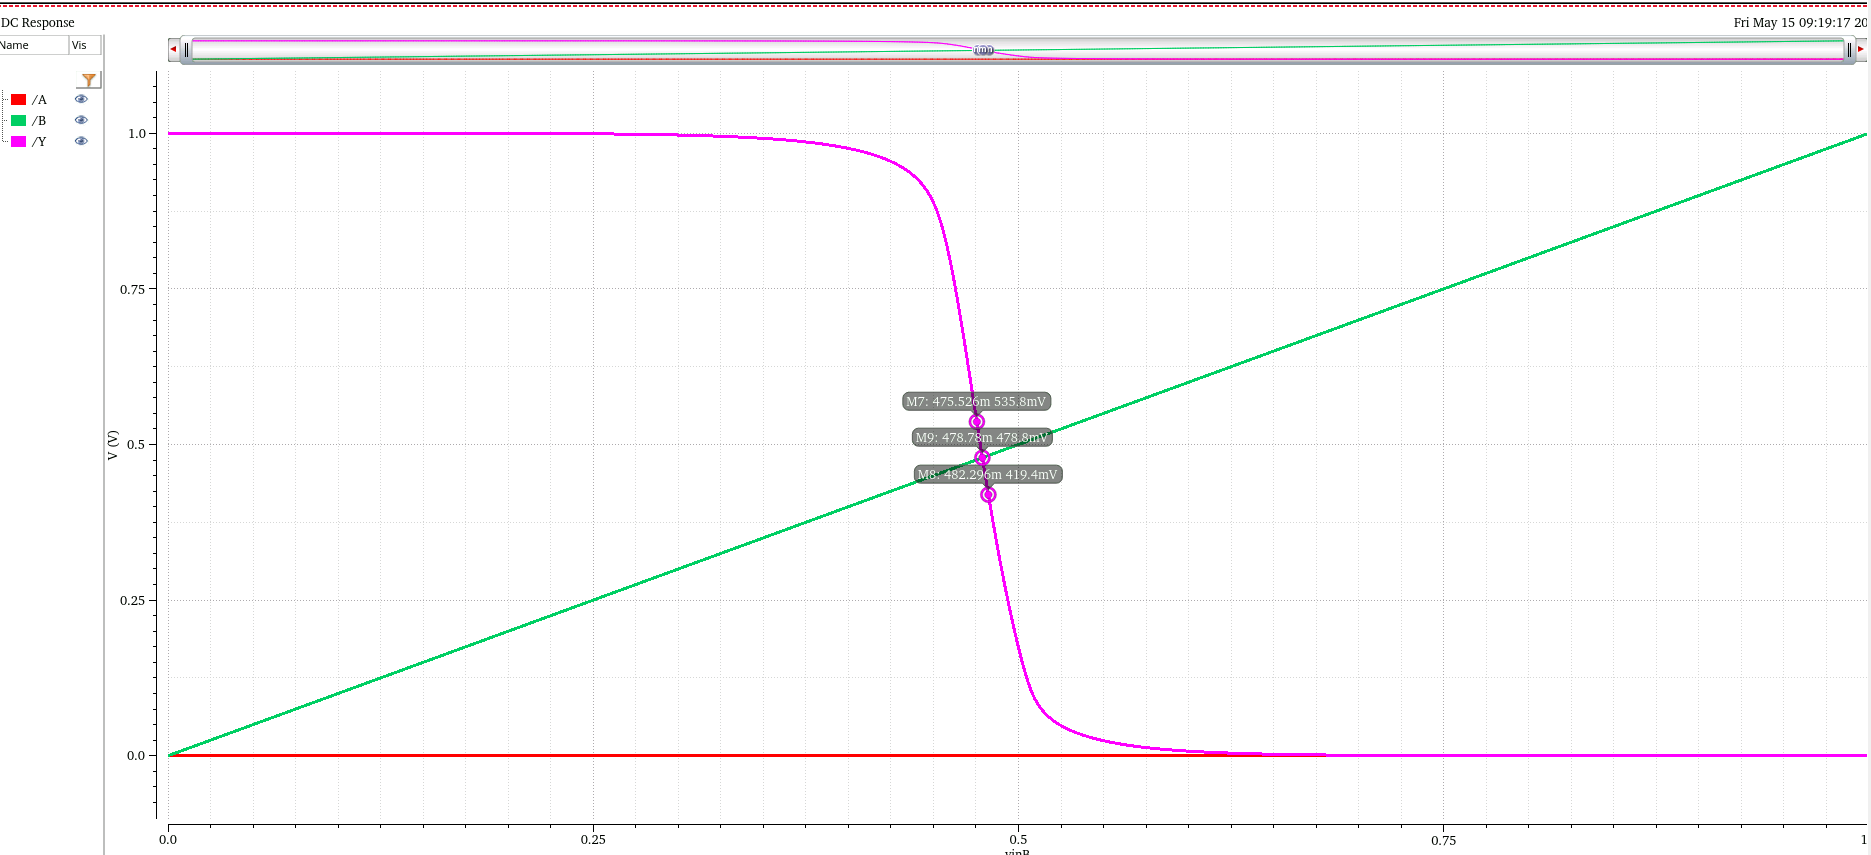
\includegraphics[width=0.45\textwidth]{nor_dc_sweep_B.png}}
        \caption{Đặc tuyến VTC của cổng NOR}
    \end{figure}
    \begin{table}[H]
        \centering
        \caption{Các thông số đặc tính tĩnh DC của cổng NOR 2 ngõ vào}
        \begin{tabular}{|c|c|c|c|c|c|c|c|c|}
        \hline
        \textbf{Case} & \textbf{State} & \textbf{$V_{IL}$ (V)} & \textbf{$V_{IH}$ (V)} & \textbf{$V_M$ (V)} & \textbf{$V_{OL}$ (V)} & \textbf{$V_{OH}$ (V)} \\ \hline
        Case 1 & A sweep, B = 0 & 0.3644 & 0.5186 & 0.4374 & 0.0001 & 0.9959  \\ \hline
        Case 2 & B sweep, A = 0 & 0.4048 & 0.5658 & 0.4789 & 0.0001 & 0.9959  \\ \hline
        \end{tabular}
    \end{table}

    \noindent\textbf{Ghi chú và giải thích các trường hợp khảo sát:}
    \begin{itemize}
        \item \textbf{Case 1 (A sweep, B = 0):} Ngõ vào B được giữ cố định ở mức logic thấp (0V), ngõ vào A quét tuyến tính từ 0V đến 1V. Lúc này, NMOS nối với B bị khóa hoàn toàn, PMOS tương ứng ở trạng thái dẫn. Cấu trúc mạch tương đương với một cổng Inverter tác động bởi ngõ vào A. Do đặc thù các transistor PMOS nối tiếp xếp chồng lên nhau làm tăng điện trở kéo lên (pull-up resistance), điểm chuyển mạch $V_M$ bị kéo dịch về phía điện áp thấp hơn.
        \item \textbf{Case 2 (B sweep, A = 0):} Ngõ vào A được giữ cố định ở mức logic thấp (0V), ngõ vào B quét tuyến tính từ 0V đến 1V. Sự bất đối xứng về vị trí sơ đồ giữa hai mạng PMOS mắc nối tiếp kéo nguồn khiến cho điện dung ký sinh và nội trở sụt áp tại điểm nút giữa hai transistor thay đổi. Kết quả mô phỏng cho thấy điểm ngưỡng chuyển mạch $V_M$ đạt 0.4789V, kéo theo sự thay đổi tương ứng của các khoảng lề nhiễu logic thấp và lề nhiễu logic cao.
    \end{itemize}

    \item \textbf{Mô phỏng Transient và Đo đạc thông số của trường hợp 1:}
    \begin{figure}[H]
        \centering
        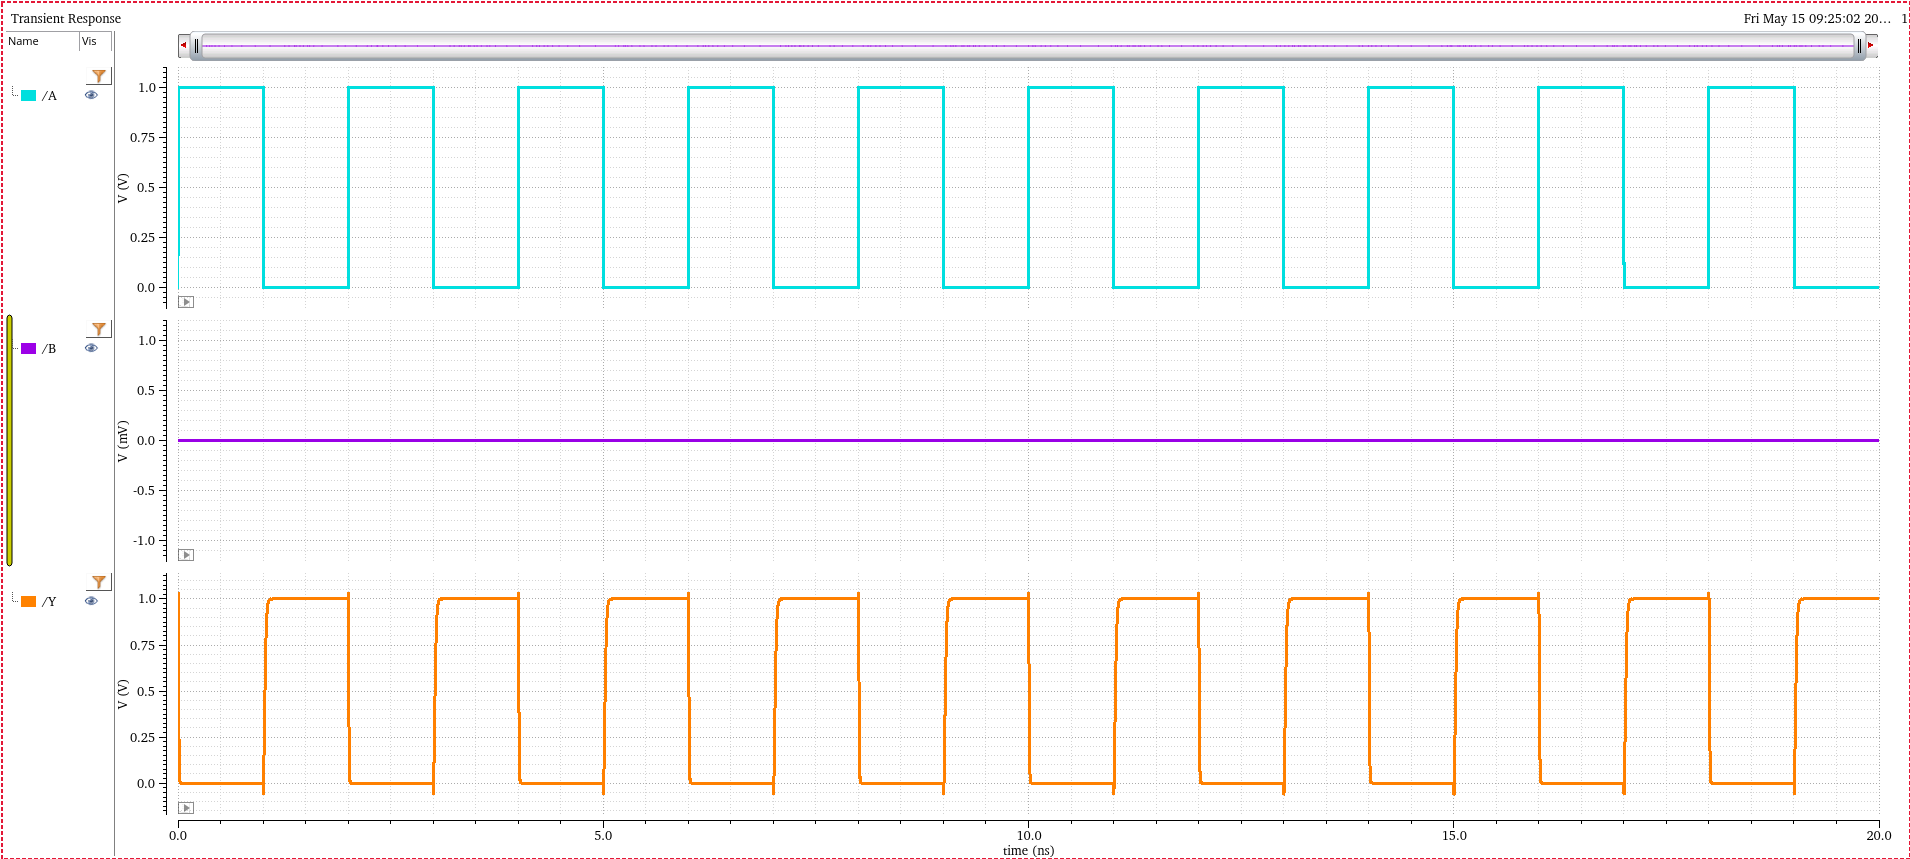
\includegraphics[width=0.8\textwidth]{nor_transient_waveforms.png}
        \caption{Kết quả mô phỏng Transient cổng NOR}
    \end{figure}
% Bảng tổng hợp kết quả từ Calculator cho TH1
    \begin{table}[H]
        \centering
        \caption{Kết quả đo đạc thông số thời gian và công suất bằng Calculator (TH1)}
        \begin{tabular}{|c|c|c|c|c|c|c|c|}
        \hline
        \textbf{$t_{rise}$} & \textbf{$t_{fall}$} & \textbf{$t_{pdr}$} & \textbf{$t_{pdf}$} & \textbf{$t_{pd}$} & \textbf{Static Pwr 0} & \textbf{Static Pwr 1} & \textbf{Dynamic Pwr} \\ 
        \textbf{(ps)} & \textbf{(ps)} & \textbf{(ps)} & \textbf{(ps)} & \textbf{(ps)} & \textbf{(nW)} & \textbf{(nW)} & \textbf{(nW)} \\ \hline
        34,42 & 12,68 & 21,63 & 7,8 & 14,3 & 0.289 & 0,0634 & 882,3 \\ \hline
        \end{tabular}
    \end{table}

    \begin{figure}[H]
        \centering
        \subfigure[Đo $t_{rise}$]{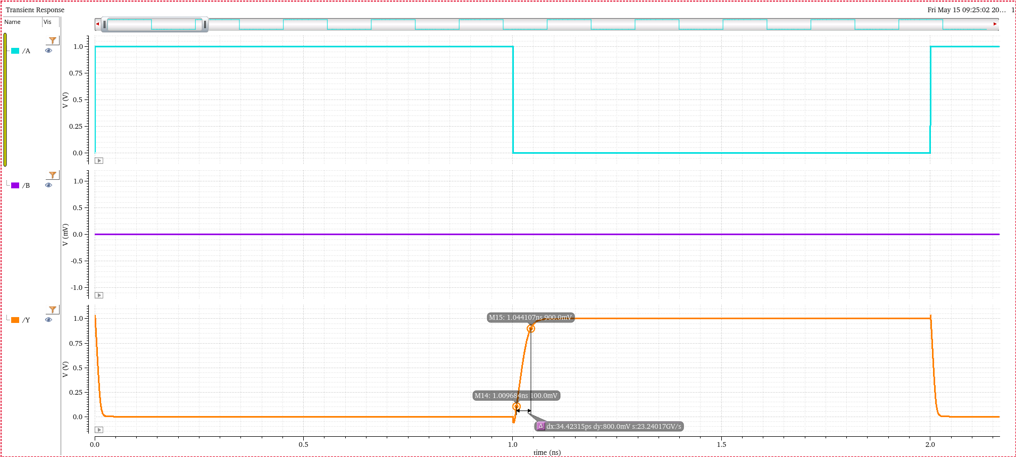
\includegraphics[width=0.6\textwidth]{nor_trise.png}}
        \subfigure[Calc $t_{rise}$]{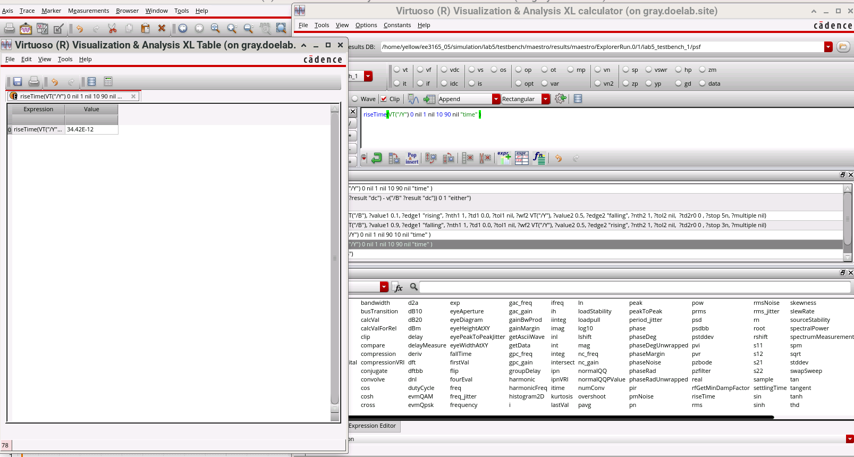
\includegraphics[width=0.5\textwidth]{nor_trise_calc.png}}
        \subfigure[Đo $t_{fall}$]{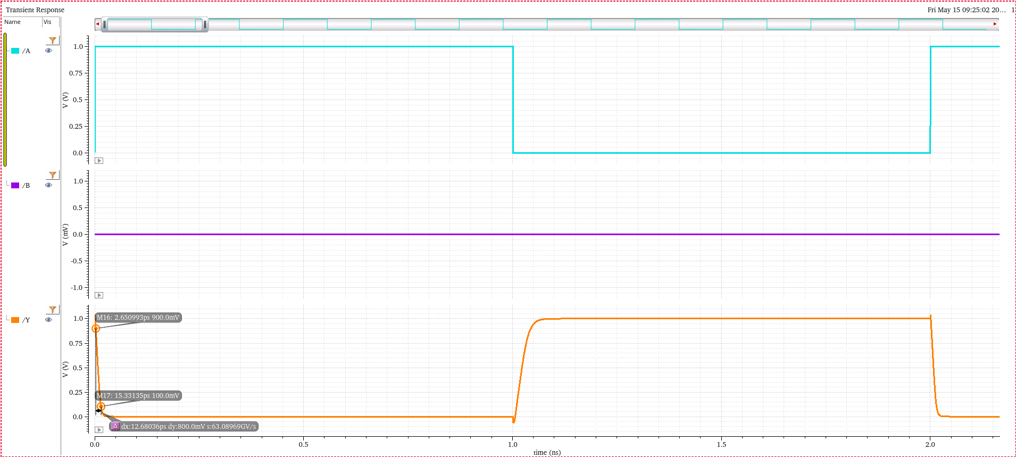
\includegraphics[width=0.6\textwidth]{nor_tfall.png}}
        \subfigure[Calc $t_{fall}$]{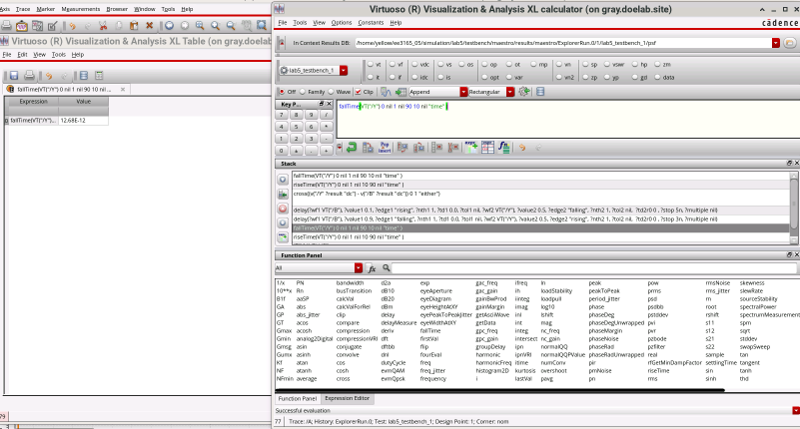
\includegraphics[width=0.5\textwidth]{nor_tfall_calc.png}}
        \caption{Thời gian cạnh lên và cạnh xuống cổng NOR}
    \end{figure}
    \begin{figure}[H]
        \centering
        \subfigure[Đo $t_{pdr}$]{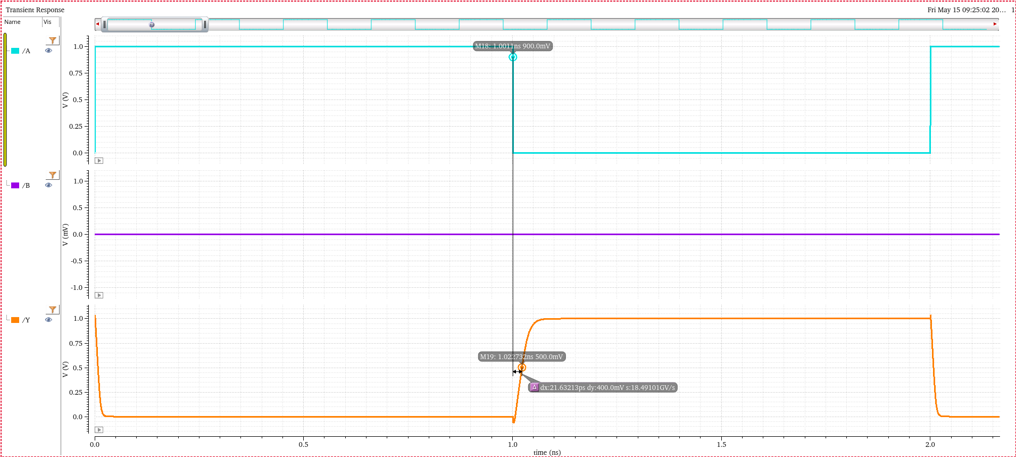
\includegraphics[width=0.5\textwidth]{nor_tpdr.png}}\hfill
        \subfigure[Calc $t_{pdr}$]{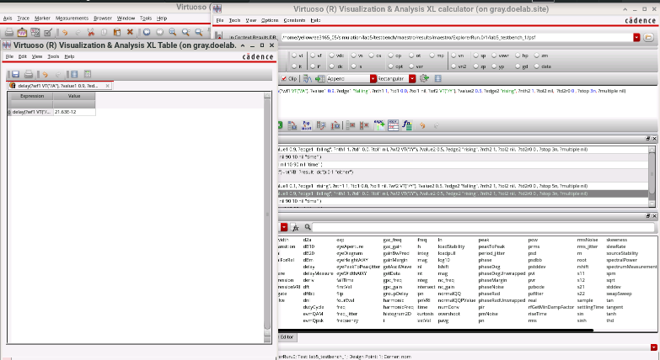
\includegraphics[width=0.40\textwidth]{nor_tpdr_calc.png}}
        \subfigure[Đo $t_{pdf}$]{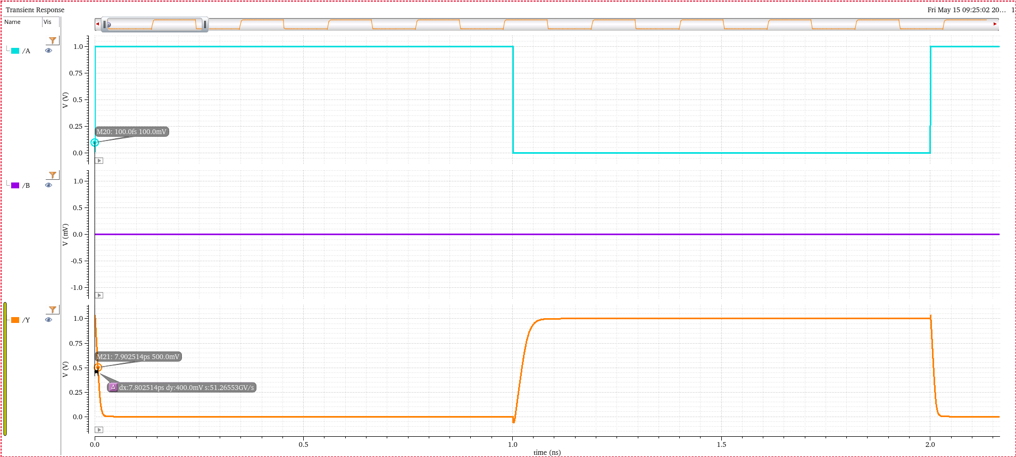
\includegraphics[width=0.5\textwidth]{nor_tpdf.png}}\hfill
        \subfigure[Calc $t_{pdf}$]{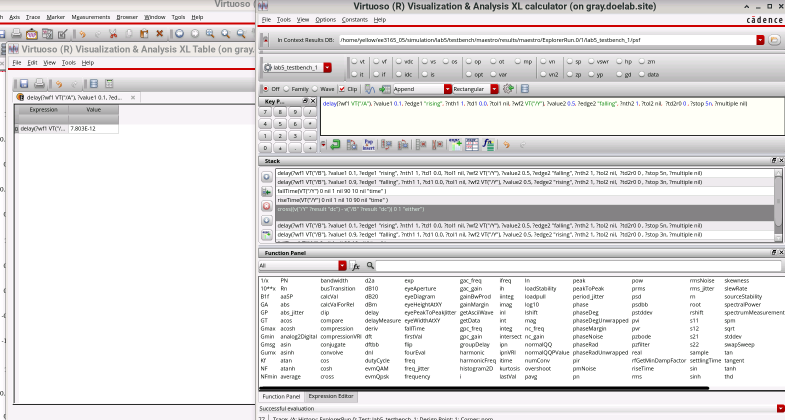
\includegraphics[width=0.40\textwidth]{nor_tpdf_calc.png}}
        \subfigure[Đo $t_{pd}$]{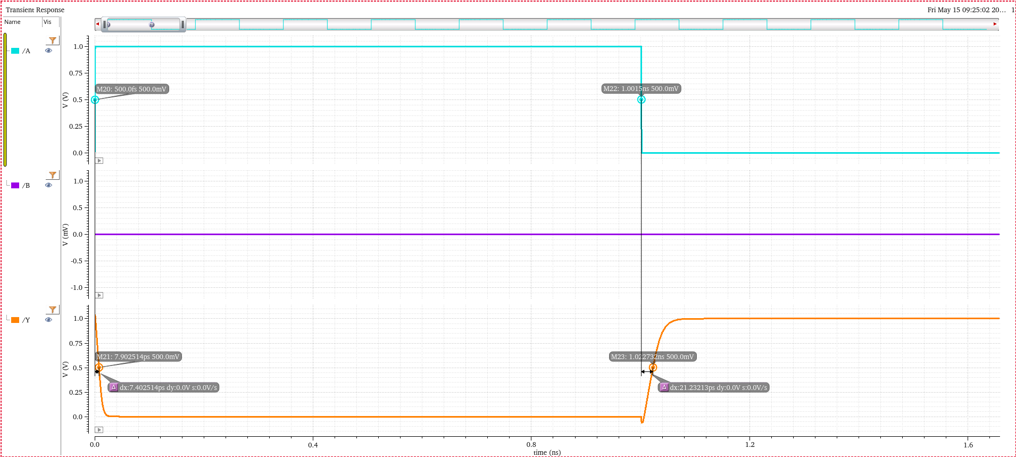
\includegraphics[width=0.5\textwidth]{nor_tpd.png}}
        \caption{Các thông số độ trễ cổng NOR}
    \end{figure}
    \begin{figure}[H]
        \centering
        \subfigure[Static Pwr (0)]{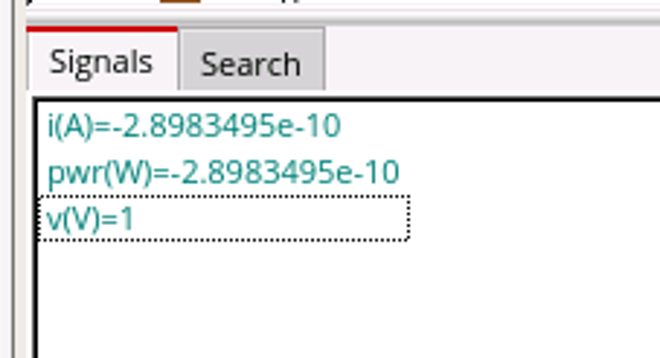
\includegraphics[width=0.6\textwidth]{nor_static_pwr_0.png}}
        \subfigure[Static Pwr (1)]{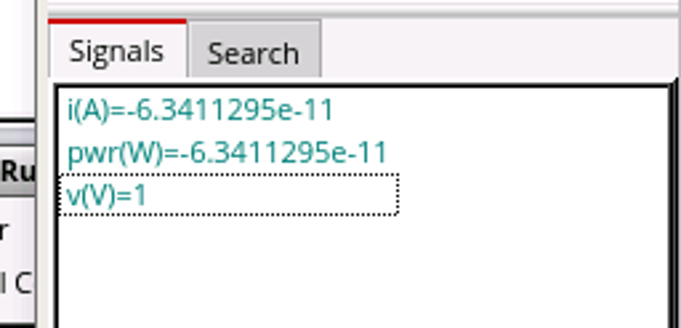
\includegraphics[width=0.6\textwidth]{nor_static_pwr_1.png}}
        \subfigure[Dynamic Pwr]{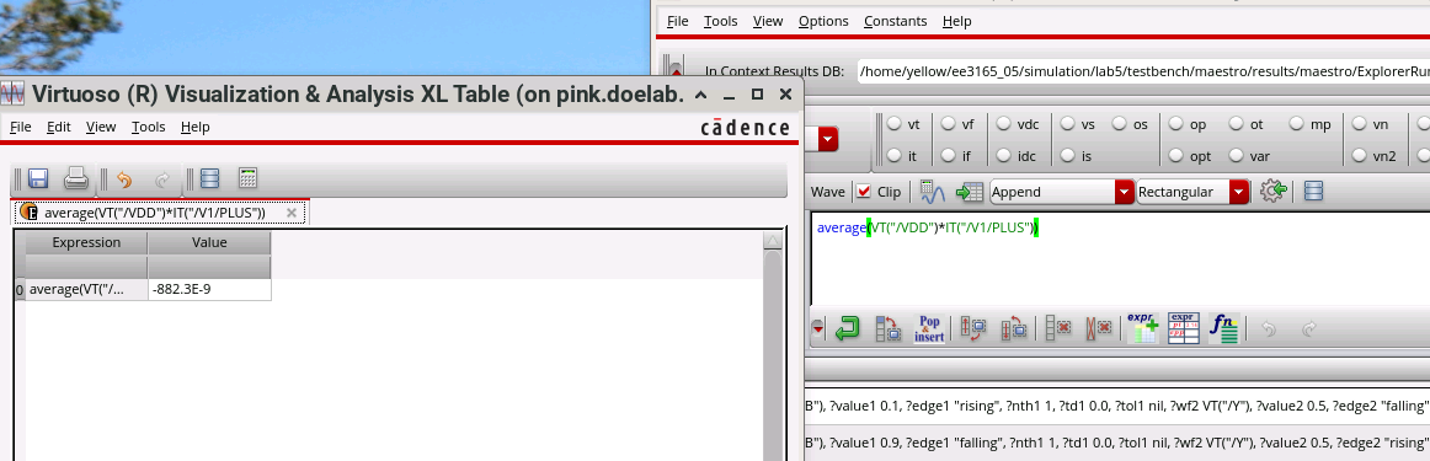
\includegraphics[width=0.6\textwidth]{nor_dynamic_pwr.png}}
        \caption{Công suất tĩnh và động cổng NOR}
    \end{figure}

    \item \textbf{Mô phỏng Transient và Đo đạc thông số của trường hợp 2:}
    \begin{figure}[H]
        \centering
        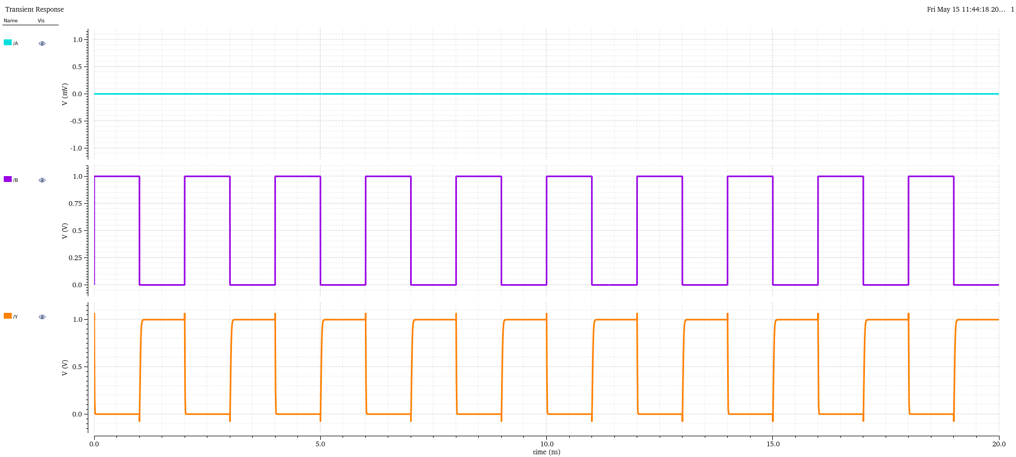
\includegraphics[width=0.8\textwidth]{nor2_transient_waveforms.png}
        \caption{Kết quả mô phỏng Transient cổng NOR}
    \end{figure}

    % Bảng tổng hợp kết quả từ Calculator cho TH2
    \begin{table}[H]
        \centering
        \caption{Kết quả đo đạc thông số thời gian và công suất bằng Calculator (TH2)}
        \begin{tabular}{|c|c|c|c|c|c|c|c|}
        \hline
        \textbf{$t_{rise}$} & \textbf{$t_{fall}$} & \textbf{$t_{pdr}$} & \textbf{$t_{pdf}$} & \textbf{$t_{pd}$} & \textbf{Static Pwr 0} & \textbf{Static Pwr 1} & \textbf{Dynamic Pwr} \\ 
        \textbf{(ps)} & \textbf{(ps)} & \textbf{(ps)} & \textbf{(ps)} & \textbf{(ps)} & \textbf{(nW)} & \textbf{(nW)} & \textbf{(nW)} \\ \hline
        34,27 & 10,98 & 19,38 & 6,7 & 12,64 & 0,3 & 0,083 & 737,7 \\ \hline
        \end{tabular}
    \end{table}
    \begin{figure}[H]
        \centering
        \subfigure[Đo $t_{rise}$]{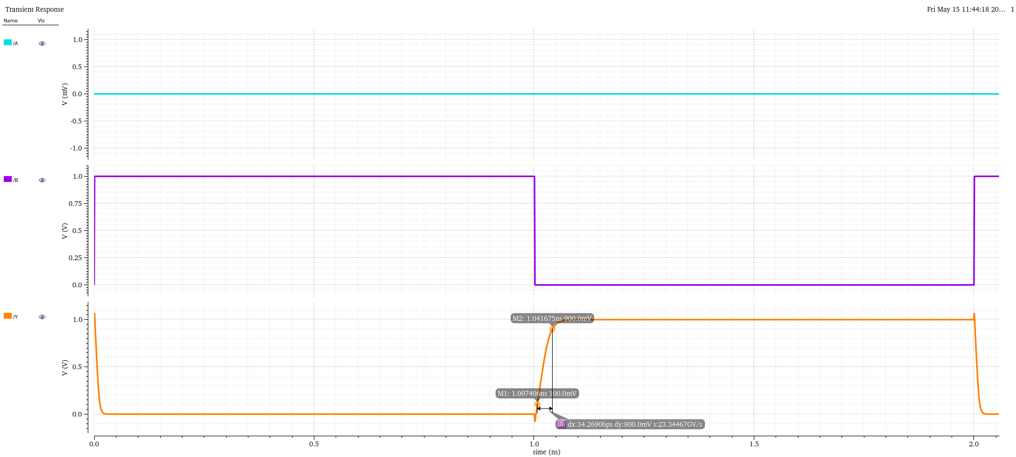
\includegraphics[width=0.6\textwidth]{nor2_trise.png}}
        \subfigure[Calc $t_{rise}$]{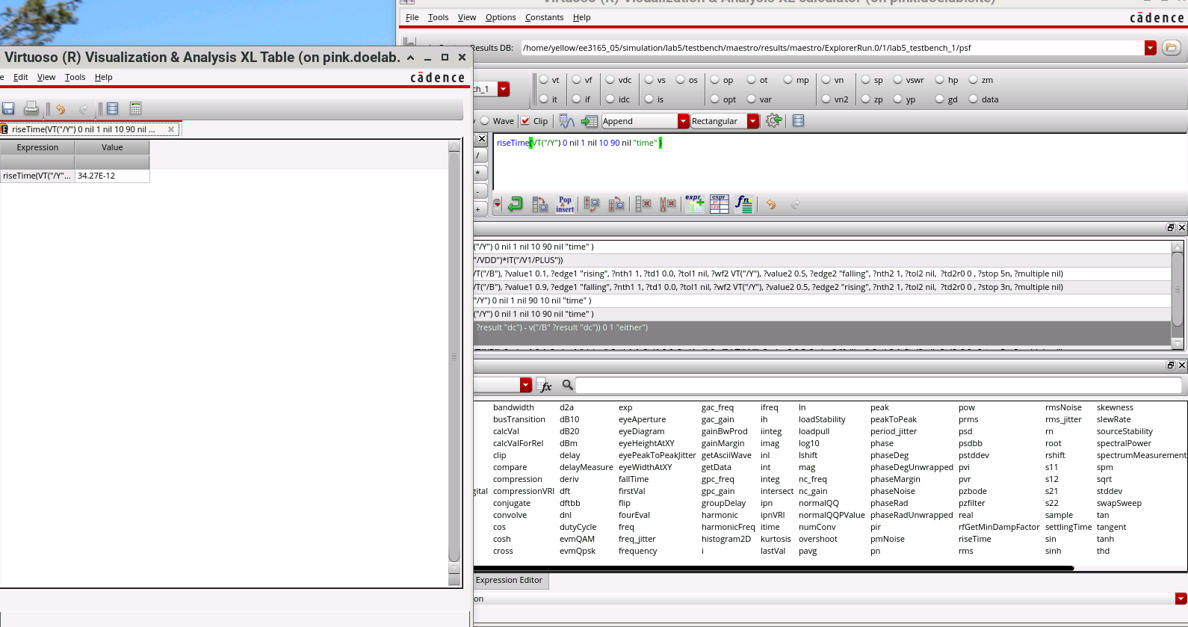
\includegraphics[width=0.48\textwidth]{nor2_trise_calc.png}}
        \subfigure[Đo $t_{fall}$]{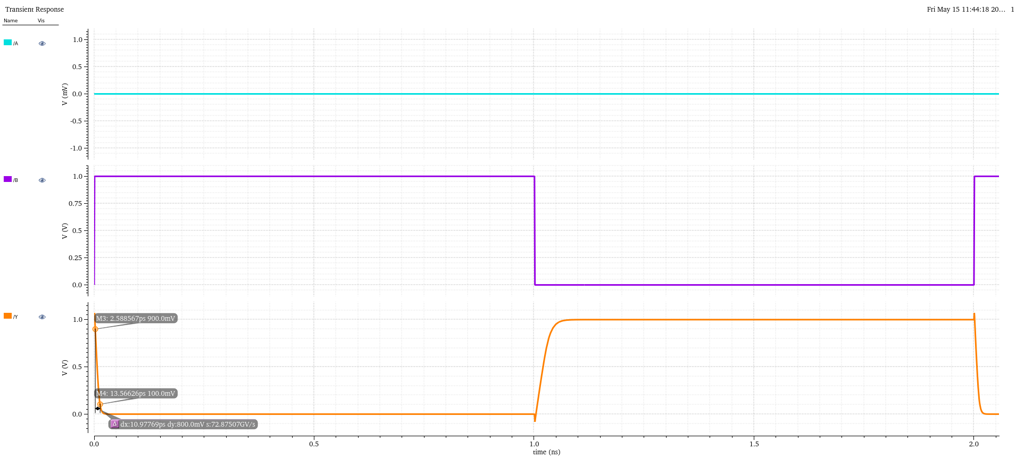
\includegraphics[width=0.6\textwidth]{nor2_tfall.png}}
        \subfigure[Calc $t_{fall}$]{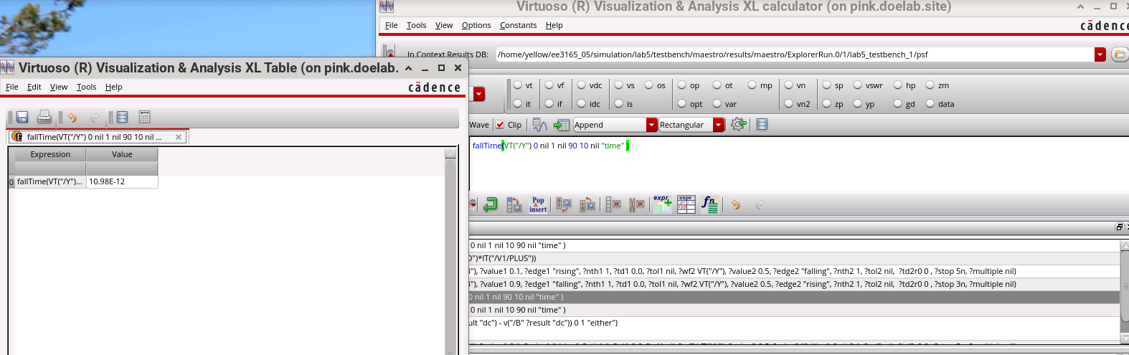
\includegraphics[width=0.48\textwidth]{nor2_tfall_calc.png}}
        \caption{Thời gian cạnh lên và cạnh xuống cổng NOR}
    \end{figure}
    \begin{figure}[H]
        \centering
        \subfigure[Đo $t_{pdr}$]{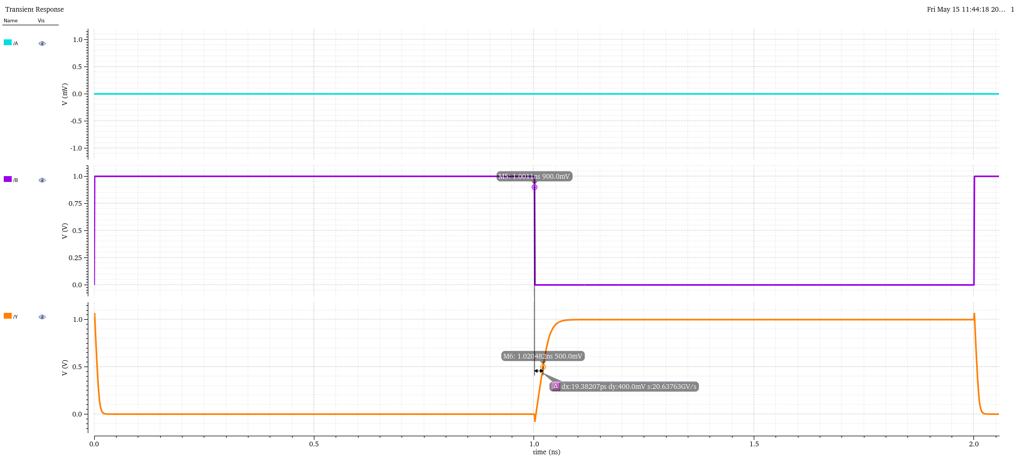
\includegraphics[width=0.6\textwidth]{nor2_tpdr.png}}
        \subfigure[Calc $t_{pdr}$]{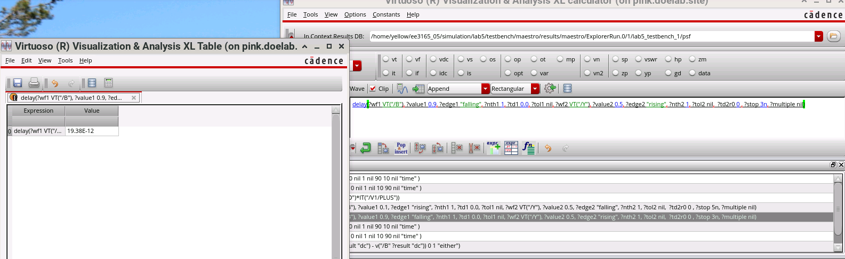
\includegraphics[width=0.48\textwidth]{nor2_tpdr_calc.png}}
        \subfigure[Đo $t_{pdf}$]{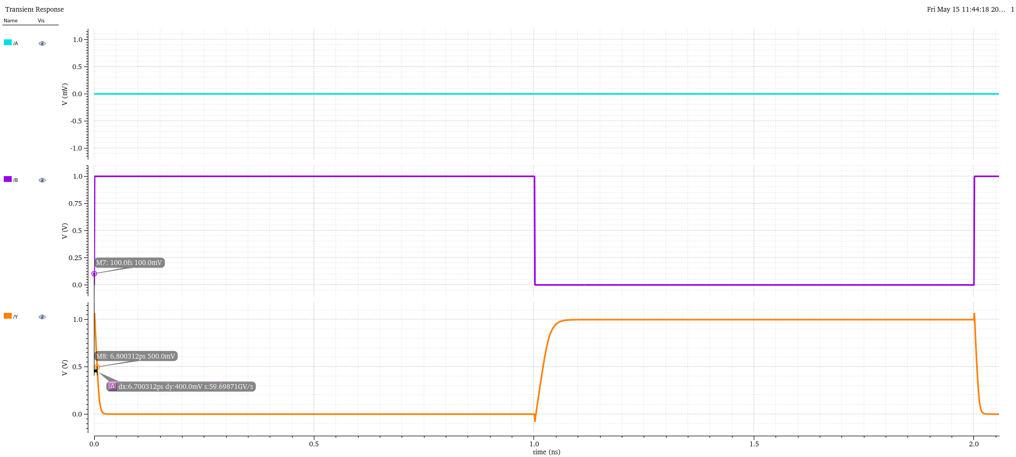
\includegraphics[width=0.6\textwidth]{nor2_tpdf.png}}
        \subfigure[Calc $t_{pdf}$]{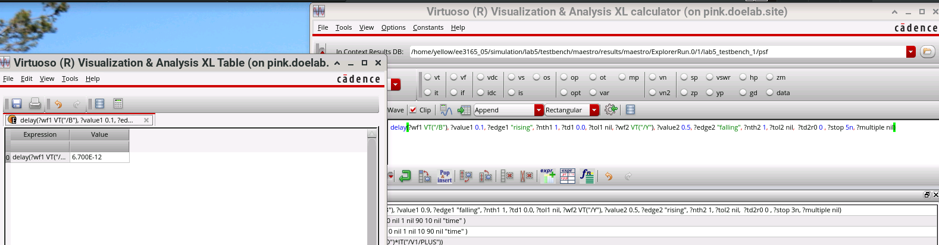
\includegraphics[width=0.48\textwidth]{nor2_tpdf_calc.png}}
        \subfigure[Đo $t_{pd}$]{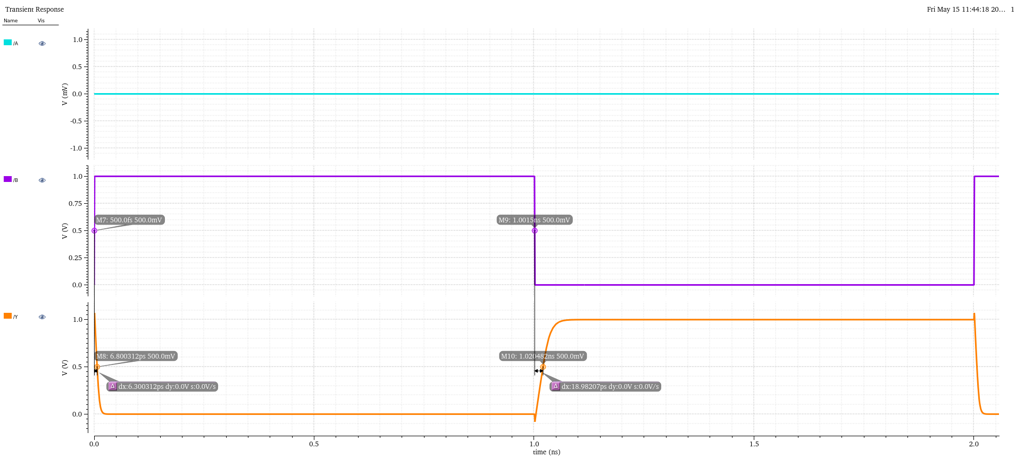
\includegraphics[width=0.6\textwidth]{nor2_tpd.png}}
        \caption{Các thông số độ trễ cổng NOR}
    \end{figure}
    \begin{figure}[H]
        \centering
        \subfigure[Static Pwr (0)]{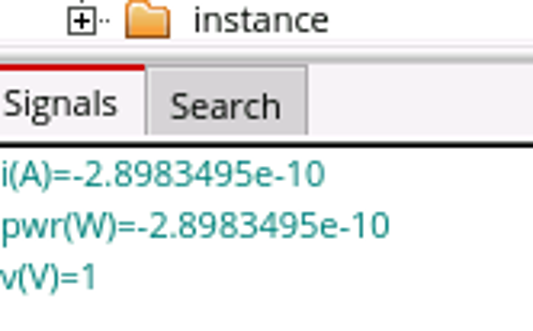
\includegraphics[width=0.6\textwidth]{nor2_static_pwr_0.png}}
        \subfigure[Static Pwr (1)]{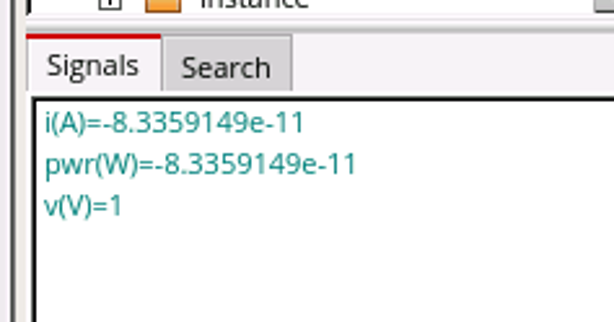
\includegraphics[width=0.6\textwidth]{nor2_static_pwr_1.png}}
        \subfigure[Dynamic Pwr]{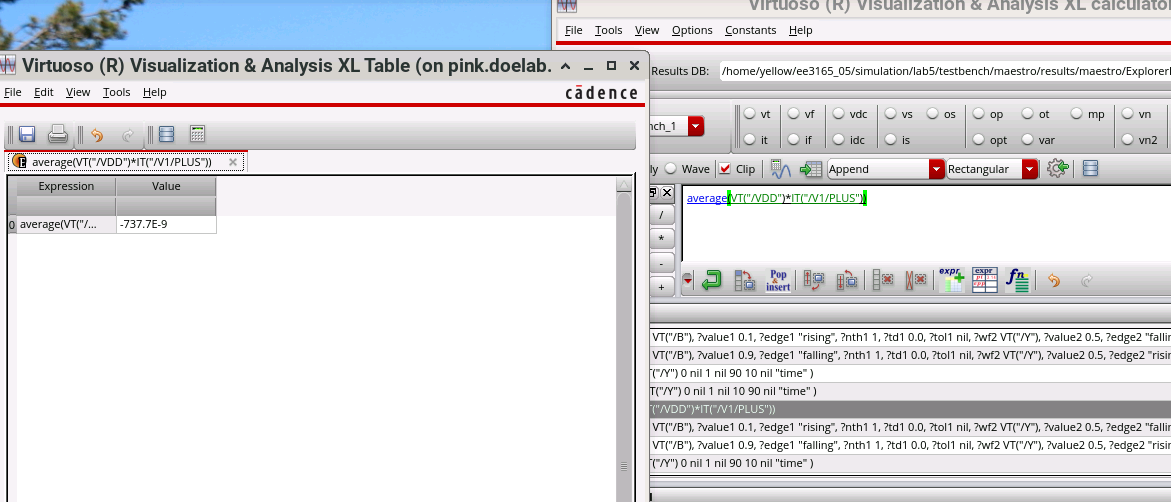
\includegraphics[width=0.6\textwidth]{nor2_dynamic_pwr.png}}
        \caption{Công suất tĩnh và động cổng NOR}
    \end{figure}

    \item \textbf{Hiệu chỉnh kích thước (Adjust $V_M = V_{DD}/2$):}

Để đạt được điện áp chuyển mạch $V_M \approx V_{DD}/2$, kích thước của transistor PMOS được tăng lên so với NMOS nhằm bù lại độ linh động hạt tải của PMOS thấp hơn so với NMOS. Bằng cách ta sẽ thay đổi giá trị Finger Width của cả 2 PMOS. Đầu tiên ta sẽ đặt biến width M vào chỗ Finger Width để quét giá trị.

    \begin{figure}[H]
        \centering
        \subfigure[Thiết lập Sweep]{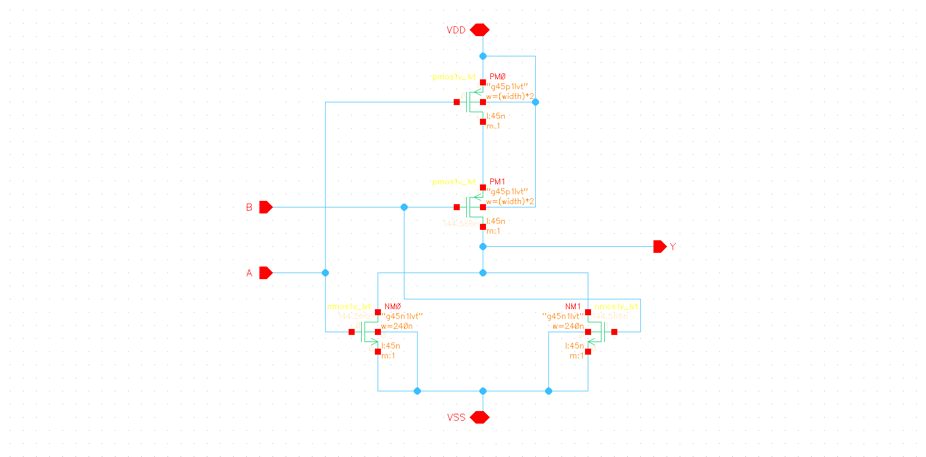
\includegraphics[width=\textwidth]{nor_sizing_setup.png}}
        \subfigure[Kết quả Sweep VTC TH1 tại width=204ns]{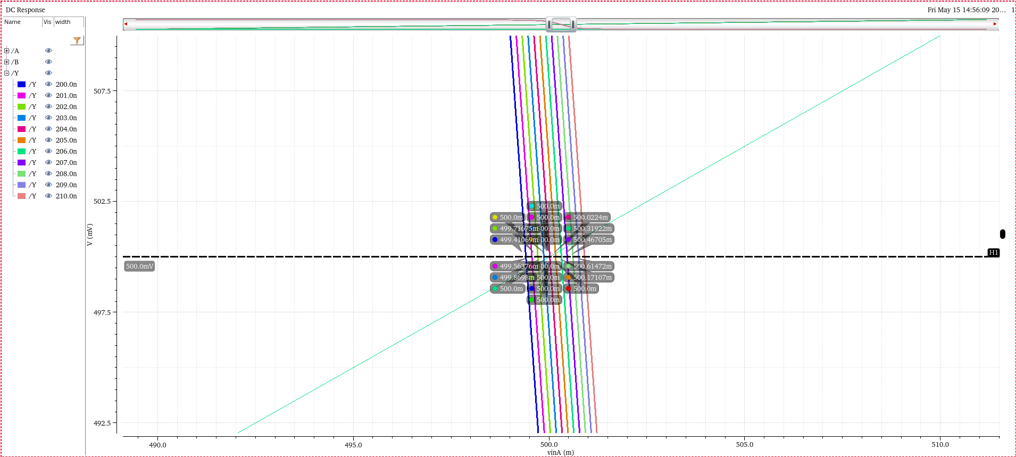
\includegraphics[width=0.65\textwidth]{nor_sizing_result1.png}}
        \subfigure[Kết quả Sweep VTC TH2 tại width=232ns]{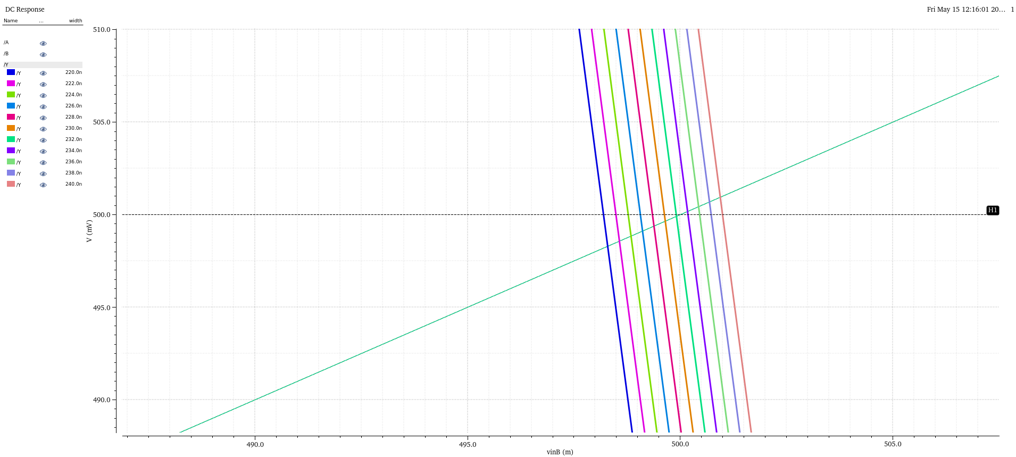
\includegraphics[width=0.65\textwidth]{nor_sizing_result2.png}}
        \caption{Hiệu chỉnh kích thước để tối ưu điểm chuyển mạch cho cổng NOR}
    \end{figure}
\end{itemize}
\newpage

% =================================================================
% EXPERIMENT 3: XOR GATE
% =================================================================
\section{Experiment 3: Circuit Design for a CMOS XOR Logic Gate}
\subsection{Cổng logic CMOS XOR}
\begin{itemize}
    \item \textbf{Bảng chân trị và Hoạt động:} (Trình bày bảng chân trị và nguyên lý cổng XOR).
    \item \textbf{Schematic và Symbol:}
    \begin{figure}[H]
        \centering
        \subfigure[Schematic XOR]{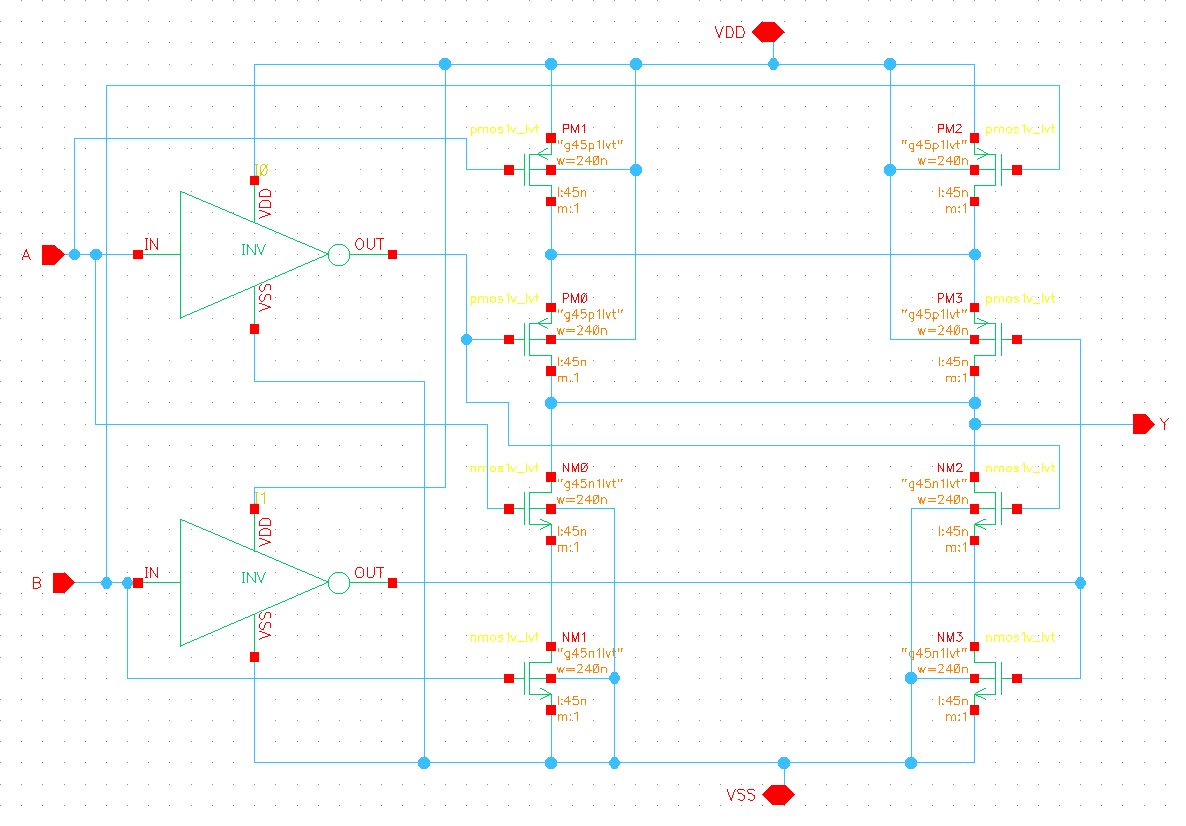
\includegraphics[width=0.45\textwidth]{xor_schematic.png}}
        \subfigure[Symbol XOR]{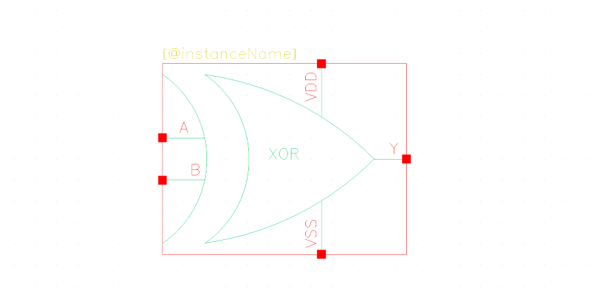
\includegraphics[width=0.45\textwidth]{xor_symbol.png}}
        \caption{Sơ đồ nguyên lý và Symbol cổng XOR}
    \end{figure}
    
    \item \textbf{Khảo sát DC (2 trường hợp):}
        \begin{enumerate}
            \item TH1: Thay đổi A, giữ B cố định.
            \item TH2: Thay đổi B, giữ A cố định.
        \end{enumerate}
    \begin{figure}[H]
        \centering
        \subfigure[DC Sweep A]{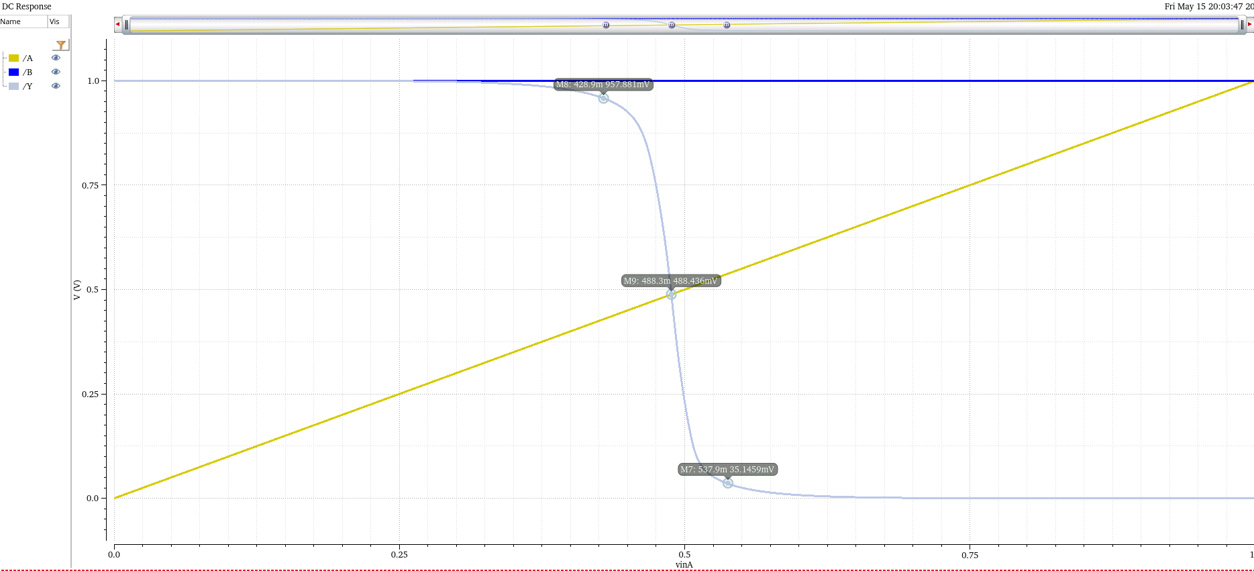
\includegraphics[width=0.45\textwidth]{xor_dc_sweep_A.png}}
        \subfigure[DC Sweep B]{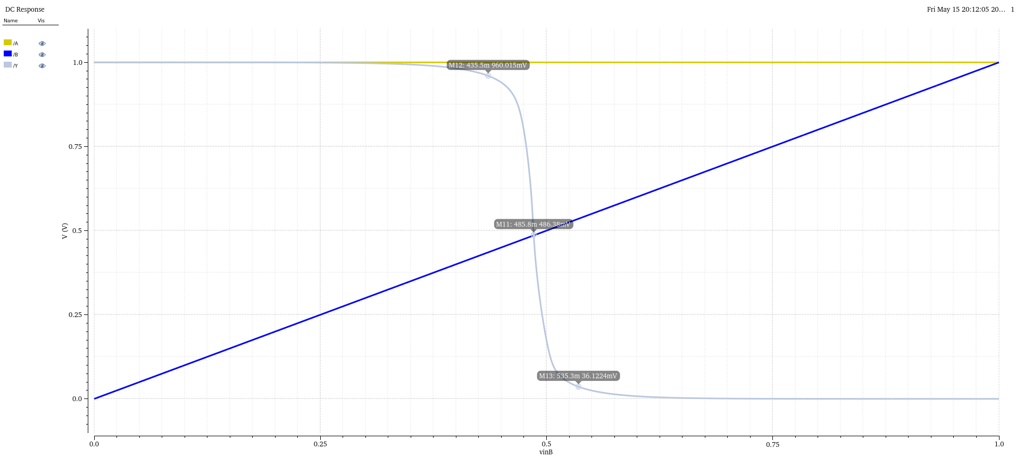
\includegraphics[width=0.45\textwidth]{xor_dc_sweep_B.png}}
        \caption{Đặc tuyến VTC của cổng XOR trong các trường hợp khảo sát}
    \end{figure}

    \begin{table}[H]
        \centering
        \caption{Các thông số đặc tính tĩnh DC của cổng XOR}
        \begin{tabular}{|c|c|c|c|c|c|c|c|c|}
        \hline
        \textbf{Case} & \textbf{State} & \textbf{$V_{IL}$ (V)} & \textbf{$V_{IH}$ (V)} & \textbf{$V_M$ (V)} & \textbf{$V_{OL}$ (V)} & \textbf{$V_{OH}$ (V)}\\ \hline
        Case 1 & A sweep, B cố định & 0,429 & 0,538 & 0,488 & 0 & 1  \\ \hline
        Case 2 & B sweep, A cố định & 0,436 & 0,535 & 0,486 & 0 & 1  \\ \hline
        \end{tabular}
    \end{table}

    \noindent\textbf{Ghi chú và giải thích các trường hợp khảo sát:}
    \begin{itemize}
        \item \textbf{Case 1:} Khảo sát đặc tính truyền đạt tĩnh khi tín hiệu ngõ vào A thay đổi tuyến tính. Cấu trúc đối xứng hoặc bất đối xứng của các đường nạp/xả nội tại quyết định độ dốc đặc tuyến và các khoảng lề nhiễu logic.
        \item \textbf{Case 2:} Khảo sát khi ngõ vào B thay đổi. Do sự phân bố vị trí các transistor trong mạng kéo lên và kéo xuống ảnh hưởng tới điện trở kênh và hiệu ứng thân, điểm ngưỡng dịch chuyển nhẹ so với Case 1.
    \end{itemize}

    \item \textbf{Mô phỏng Transient và Đo đạc thông số:}
    \begin{figure}[H]
        \centering
        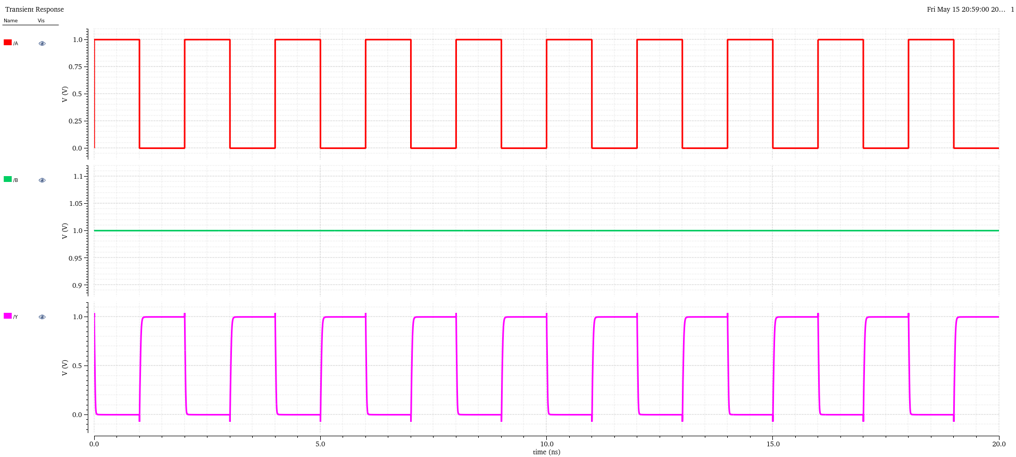
\includegraphics[width=0.8\textwidth]{xor_transient_waveforms.png}
        \caption{Kết quả mô phỏng Transient cổng XOR}
    \end{figure}

    \begin{table}[H]
        \centering
        \caption{Kết quả đo đạc thông số định thời và công suất bằng Calculator cho XOR}
        \begin{tabular}{|c|c|c|c|c|c|c|h|}
        \hline
        \textbf{$t_{rise}$} & \textbf{$t_{fall}$} & \textbf{$t_{pdr}$} & \textbf{$t_{pdf}$} & \textbf{$t_{pd}$} & \textbf{Static Pwr 0} & \textbf{Static Pwr 1} & \textbf{Dynamic Pwr} \\ 
        \textbf{(ps)} & \textbf{(ps)} & \textbf{(ps)} & \textbf{(ps)} & \textbf{(ps)} & \textbf{(nW)} & \textbf{(nW)} & \textbf{($\mu$W)} \\ \hline
        38,58 & 28,3 & 19,97 & 15,46 & 17,315 & 0,47 & 0,5 & 1,22 \\ \hline
        \end{tabular}
    \end{table}

    \begin{figure}[H]
        \centering
        \subfigure[Đo $t_{rise}$]{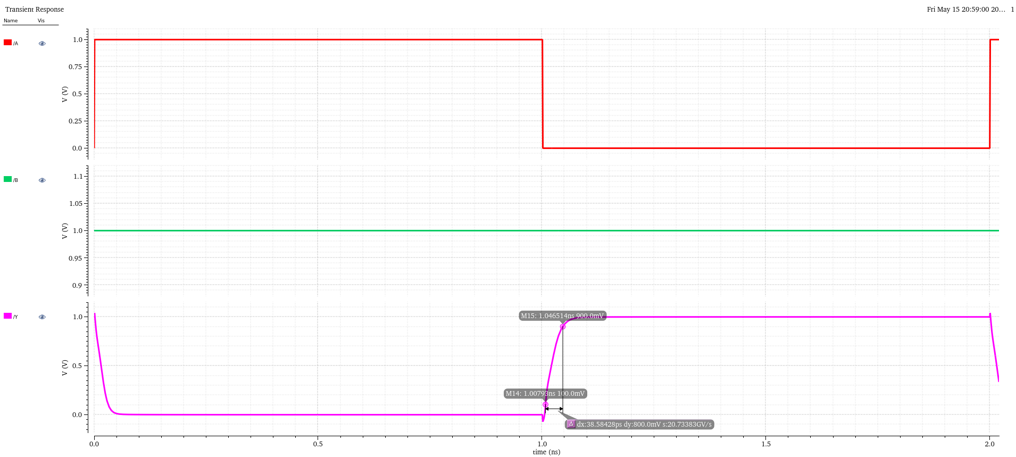
\includegraphics[width=0.5\textwidth]{xor_trise.png}}
        \subfigure[Calc $t_{rise}$]{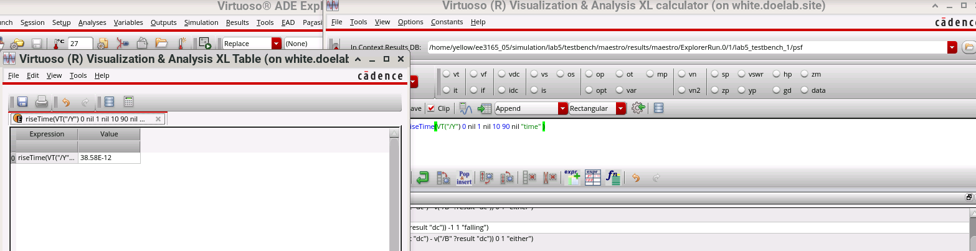
\includegraphics[width=0.5\textwidth]{xor_trise_calc.png}}
        \subfigure[Đo $t_{fall}$]{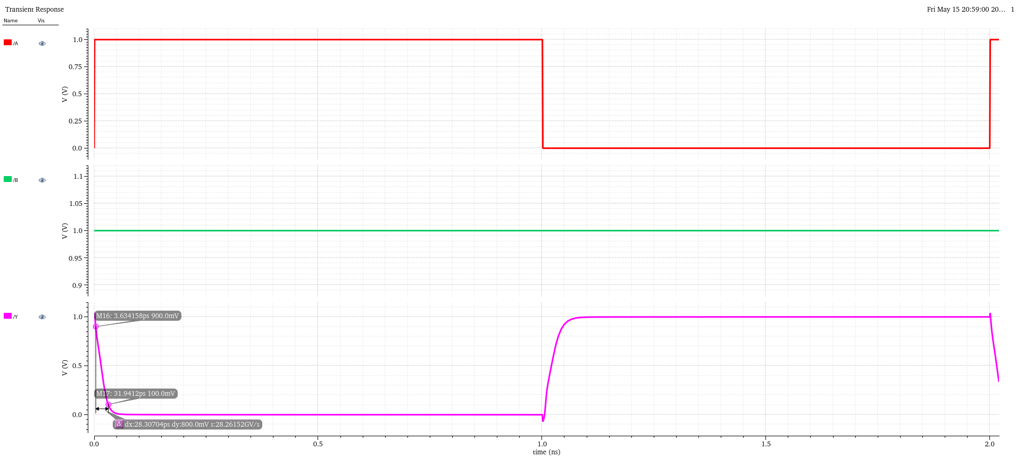
\includegraphics[width=0.5\textwidth]{xor_tfall.png}}
        \subfigure[Calc $t_{fall}$]{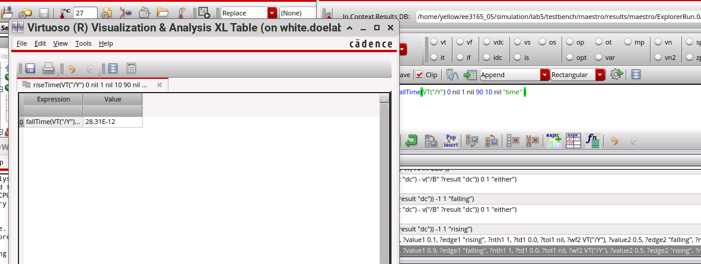
\includegraphics[width=0.5\textwidth]{xor_tfall_calc.png}}
        \caption{Thời gian cạnh lên và cạnh xuống cổng XOR kèm Calculator}
    \end{figure}
    \begin{figure}[H]
        \centering
        \subfigure[Đo $t_{pdr}$]{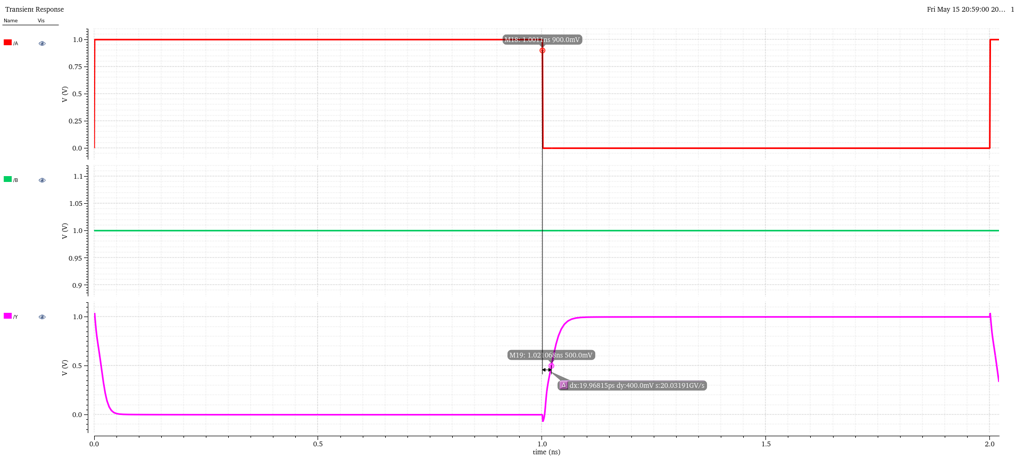
\includegraphics[width=0.5\textwidth]{xor_tpdr.png}}
        \subfigure[Calc $t_{pdr}$]{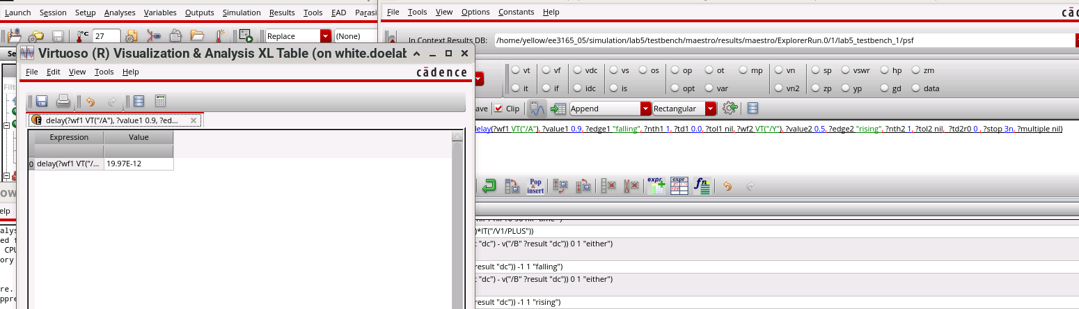
\includegraphics[width=0.5\textwidth]{xor_tpdr_calc.png}}
        \subfigure[Đo $t_{pdf}$]{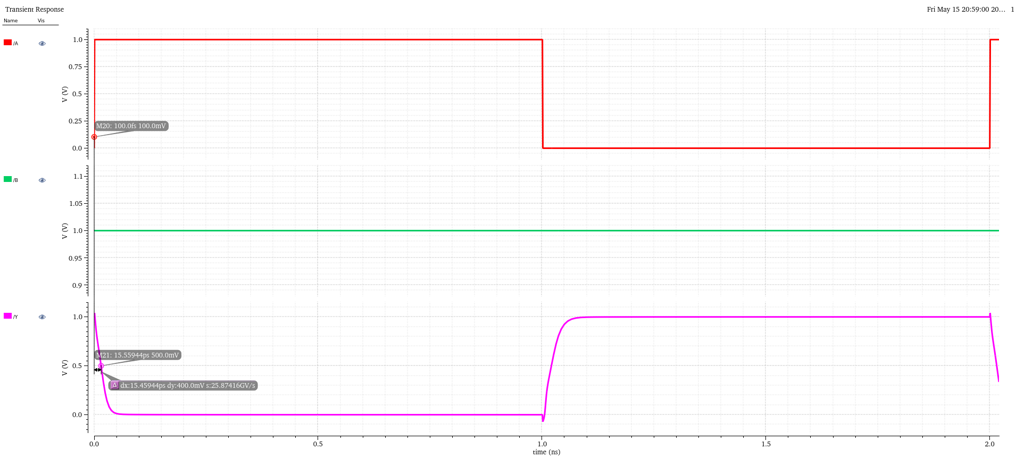
\includegraphics[width=0.5\textwidth]{xor_tpdf.png}}
        \subfigure[Calc $t_{pdf}$]{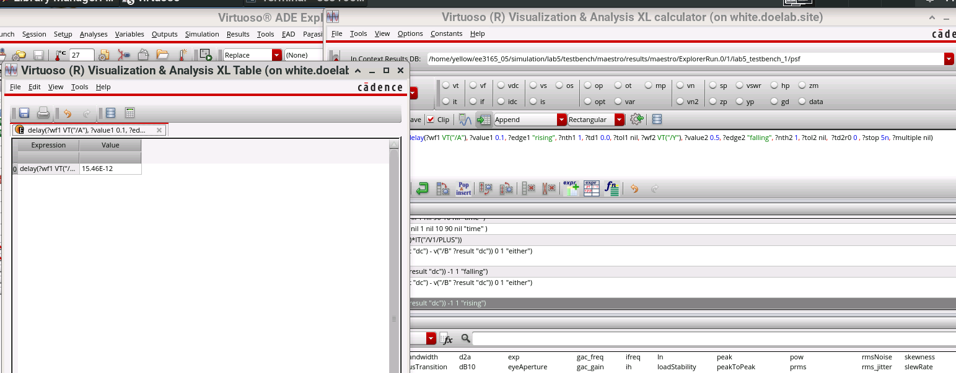
\includegraphics[width=0.5\textwidth]{xor_tpdf_calc.png}}
        \subfigure[Đo $t_{pd}$]{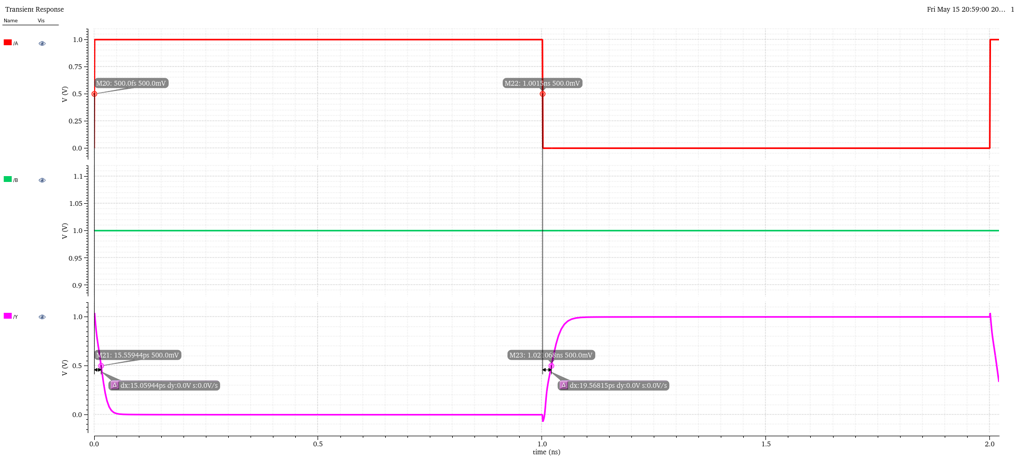
\includegraphics[width=0.5\textwidth]{xor_tpd.png}}
        \caption{Các thông số độ trễ cổng XOR kèm Calculator}
    \end{figure}
    \begin{figure}[H]
        \centering
        \subfigure[Static Pwr (0)]{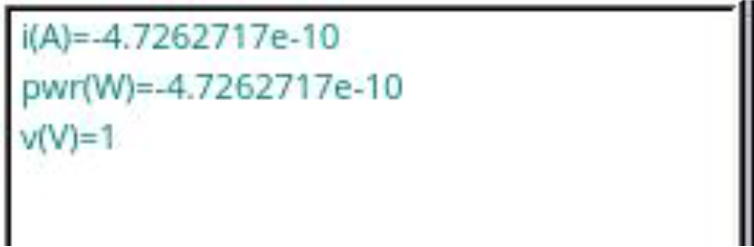
\includegraphics[width=0.52\textwidth]{xor_static_pwr_0.png}}
        \subfigure[Static Pwr (1)]{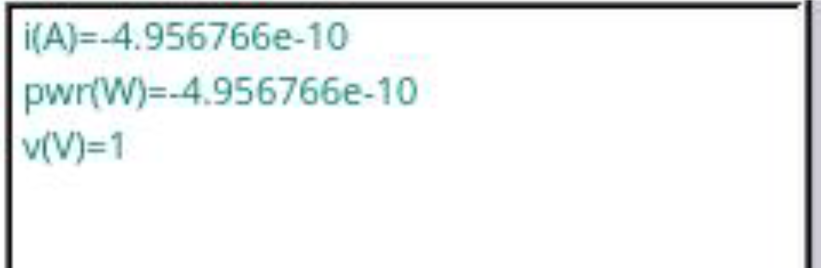
\includegraphics[width=0.5\textwidth]{xor_static_pwr_1.png}}
        \subfigure[Dynamic Pwr]{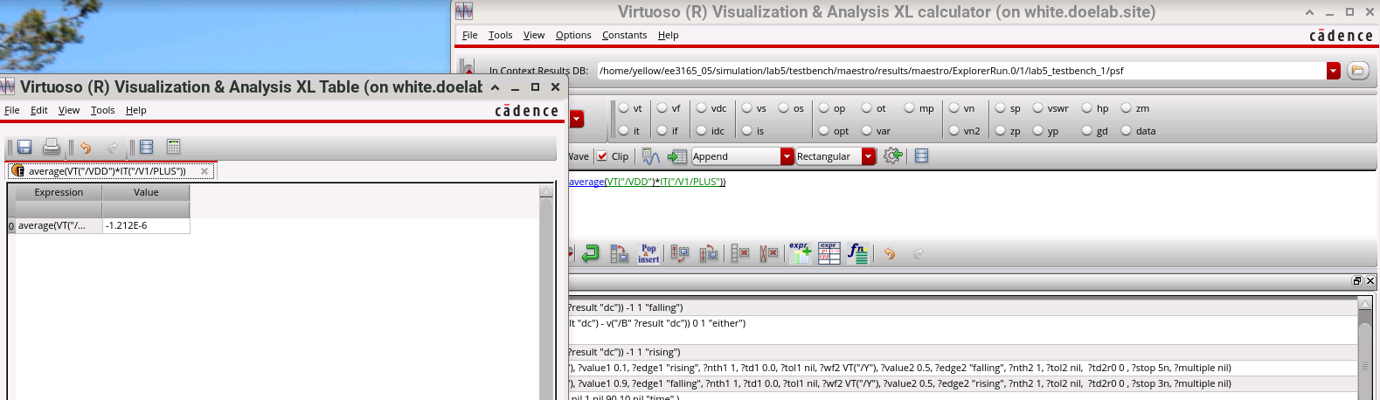
\includegraphics[width=0.52\textwidth]{xor_dynamic_pwr.png}}
        \caption{Công suất tĩnh và động cổng XOR}
    \end{figure}
\end{itemize}

\textbf{Thiết kế cổng logic CMOS XNOR từ cổng XOR ở trên.}
\begin{itemize}
\item \textbf{Schematic và Symbol:}
    \begin{figure}[H]
        \centering
        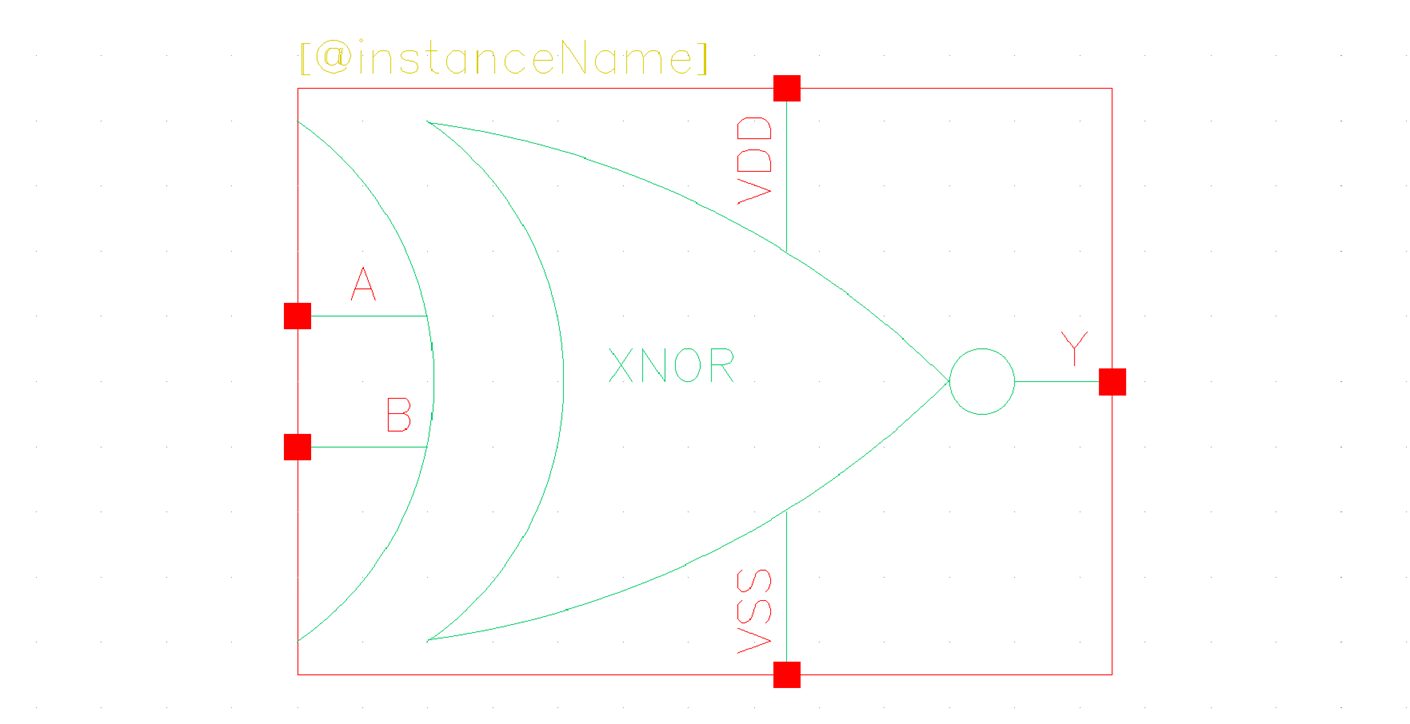
\includegraphics[width=0.5\textwidth]{1.png}
        \caption{Symbol của XNOR}
    \end{figure}
    \begin{figure}[H]
        \centering
        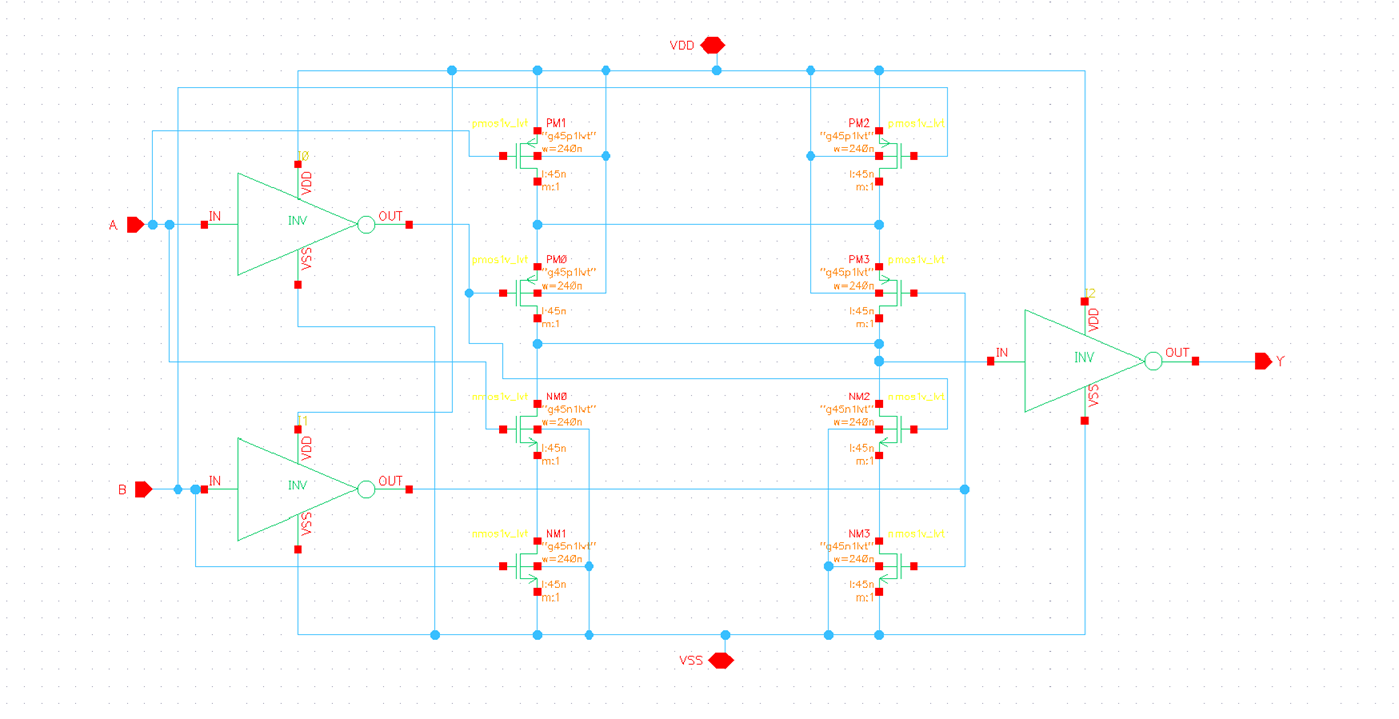
\includegraphics[width=1\textwidth]{2.png}
        \caption{Schematic của XNOR}
    \end{figure}

    \item \textbf{Mô phỏng Transient và khảo sát các thông số đặc tính năng lượng, định thời:}
    
    % Hình 1: Transient Analysis
    \begin{figure}[H]
        \centering
        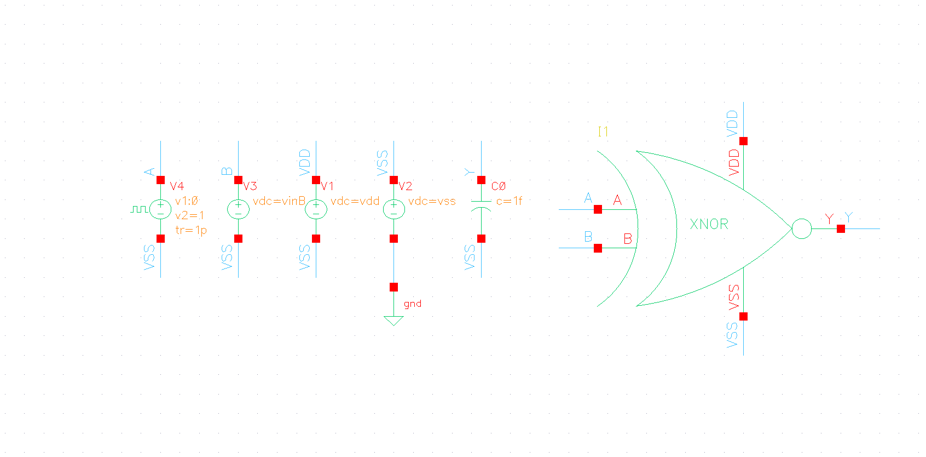
\includegraphics[width=\textwidth]{xnor_schematic.png}
        \caption{Kết quả mô phỏng Transient của cổng XNOR (Transient analysis of XNOR gate)}
    \end{figure}
    \begin{figure}[H]
        \centering
        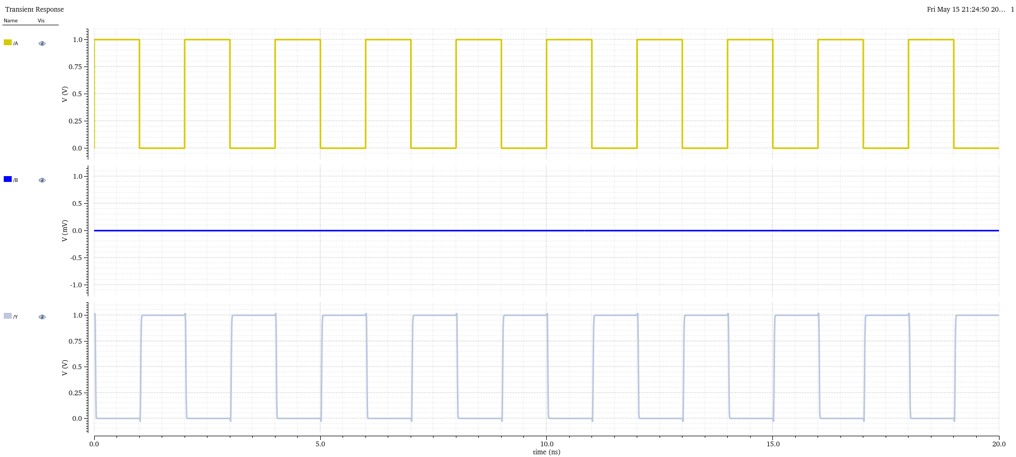
\includegraphics[width=0.8\textwidth]{xnor_transient_waveforms.png}
        \caption{Kết quả mô phỏng Transient của cổng XNOR (Transient analysis of XNOR gate)}
    \end{figure}
    \item \textbf{Nhận xét và phân tích chuyên sâu về sự khác biệt giữa cổng NOR và cổng XNOR:}
\end{itemize}
Dựa trên các kết quả mô phỏng đặc tính tĩnh (DC) và đặc tính động (Transient), ta có các đánh giá định tính và định lượng về sự khác biệt bản chất giữa cấu trúc tế bào logic tiêu chuẩn NOR và XNOR:
\begin{itemize}
    \item \textbf{Cấu trúc liên kết mạch và Số lượng Transistor:} 
    Cổng NOR 2 ngõ vào sử dụng cấu trúc CMOS tĩnh bổ sung cơ bản chỉ bao gồm 4 transistor (2 PMOS mắc nối tiếp ở mạng kéo lên PUN và 2 NMOS mắc song song ở mạng kéo xuống PDN). Ngược lại, cổng XNOR là một cấu trúc phức hợp, đòi hỏi số lượng bóng bán dẫn lớn hơn rất nhiều (thường từ 8 đến 12 transistor tùy thuộc vào việc sử dụng cấu trúc logic tĩnh hoàn toàn hay cấu trúc cổng truyền). Việc có mật độ transistor cao dẫn đến số lượng nút mạch nội tại tăng lên, làm tăng đáng kể dung kháng ký sinh tổng thể của cổng XNOR so với NOR.
    
    \item \textbf{Đặc tính tĩnh và Ngưỡng chuyển mạch $V_M$:} 
    Đối với cổng NOR, đặc tuyến chuyển vị điện áp VTC tuân theo dạng dốc đơn điệu cơ bản, trong đó điểm chuyển mạch $V_M$ bị ảnh hưởng nặng bởi hiệu ứng xếp chồng của mạng PMOS nối tiếp. Đối với XNOR, đặc tính tĩnh phức tạp hơn rất nhiều do ngõ ra không đơn điệu phụ thuộc vào một ngõ vào đơn lẻ mà phụ thuộc vào hàm tương quan giữa hai tín hiệu ngõ vào (đồng pha hoặc ngược pha). Do đó, đồ thị VTC của XNOR thay đổi hoàn toàn cấu trúc tùy thuộc vào kịch bản phối hợp mức logic nền của ngõ vào còn lại, khiến việc thiết lập Sizing hình học để đạt điểm đối xứng lý tưởng $V_M = V_{DD}/2$ phức tạp hơn cổng NOR.
    
    \item \textbf{Đặc tính động và Thời gian trễ truyền dẫn ($t_{pd}$):} 
    Mạch kéo lên của cổng NOR bị giới hạn tốc độ ở cạnh lên ($t_{rise}$) do độ linh động hạt tải của PMOS thấp kết hợp với cấu trúc mắc nối tiếp. Tuy nhiên, đường trễ tới hạn của cổng XNOR lại kéo dài hơn do tín hiệu ngõ vào phải đi qua các tầng nghịch lưu nội bộ để tạo ra các tín hiệu đảo ($\overline{A}, \overline{B}$) trước khi kích thích tầng logic quyết định phía sau. Sự trễ pha giữa tín hiệu gốc và tín hiệu đảo nội tại khiến tổng thời gian trễ truyền dẫn trung bình $t_{pd}$ của cổng XNOR lớn hơn hẳn so với cổng NOR đơn tầng.
    
    \item \textbf{Công suất tiêu thụ:} 
    Do hệ số hoạt động chuyển mạch của các nút nội tại trong XNOR cao hơn, mức tiêu thụ năng lượng của nó vượt trội so với NOR. Cổng XNOR tiêu thụ cả công suất tĩnh (do dòng rò qua nhiều transistor hơn) lẫn công suất động (do quá trình nạp/xả liên tục của các tụ ký sinh nội tại tại các nút nghịch lưu đảo pha) lớn hơn cổng NOR. Ngoài ra, do tồn tại độ lệch thời gian giữa tín hiệu thẳng và tín hiệu đảo trong mạch, cổng XNOR xuất hiện các dòng ngắn mạch dạng xung nhọn trong giai đoạn quá độ nhiều hơn, làm tăng tổng công suất tiêu thụ của linh kiện.
\end{itemize}


% =================================================================
% EXPERIMENT 4: MUX CIRCUIT
% =================================================================
\newpage
\section{Experiment 4: Circuit Design for a CMOS MUX Circuit}

\subsection{MUX Topology 1 (MUX Đảo)}
\begin{itemize}
    \item \textbf{Schematic và Symbol:}.
    \begin{figure}[H]
        \centering
        \subfigure[Schematic MUX1]{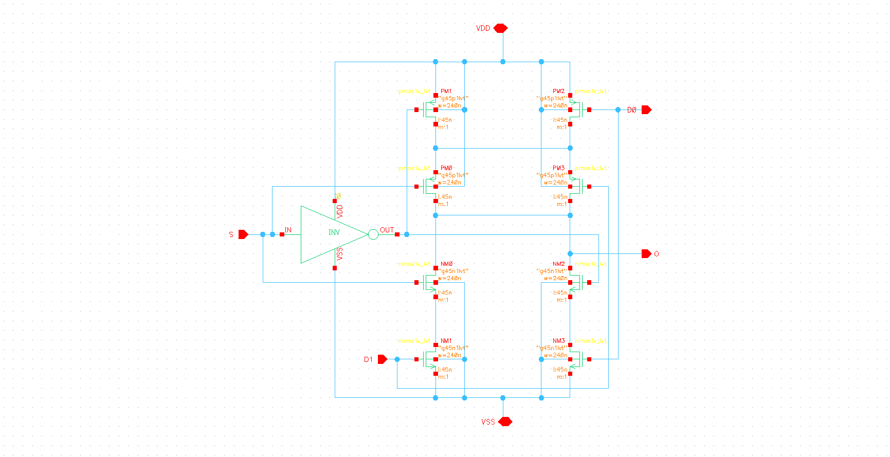
\includegraphics[width=0.9\textwidth]{mux1_schematic.png}}
        \subfigure[Schematic MUX1]{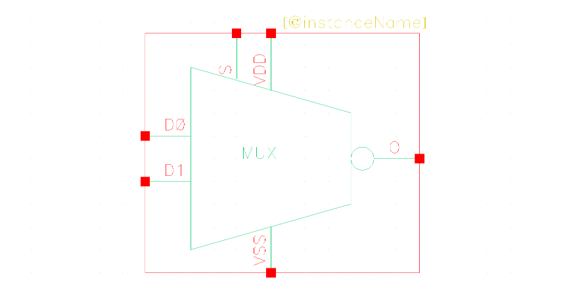
\includegraphics[width=0.6\textwidth]{mux1_symbol.png}}
        \caption{Sơ đồ nguyên lý và Symbol của MUX1}
    \end{figure}

    \item \textbf{Khảo sát DC (4 trường hợp đầy đủ):}
        \begin{enumerate}
            \item TH1: Thay đổi D0 ($S=0, D1=1$).
            \item TH2: Thay đổi D0 ($S=1, D1=1$).
            \item TH3: Thay đổi D1 ($S=0, D0=1$).
            \item TH4: Thay đổi D1 ($S=1, D0=1$).
        \end{enumerate}
    \begin{figure}[H]
        \centering
        \subfigure[DC Sweep TH1]{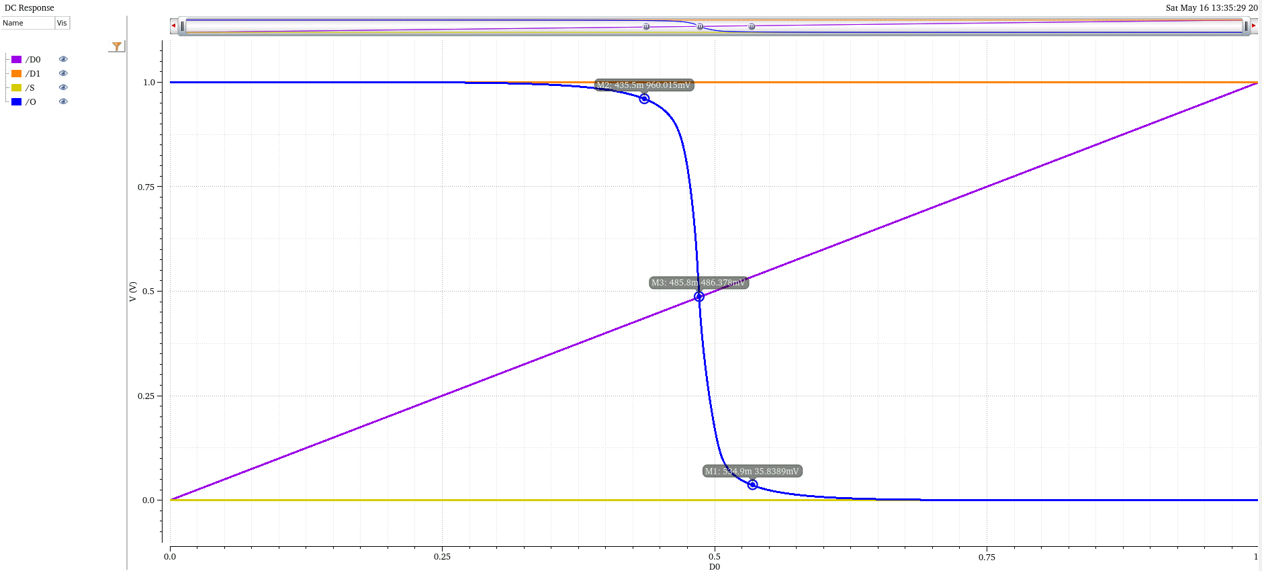
\includegraphics[width=0.6\textwidth]{mux1_dc_sweep_D0.png}}
        \subfigure[DC Sweep TH2]{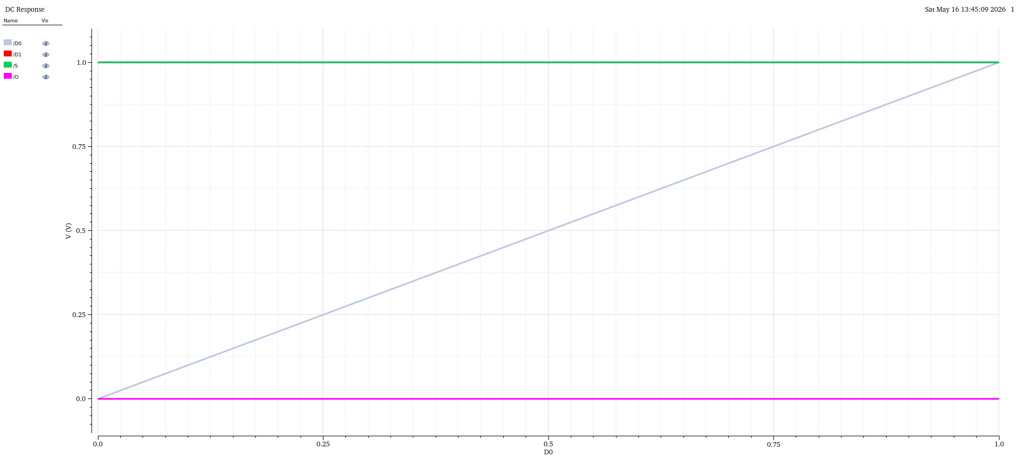
\includegraphics[width=0.6\textwidth]{mux1_dc_sweep_D1.png}}
        \subfigure[DC Sweep TH3]{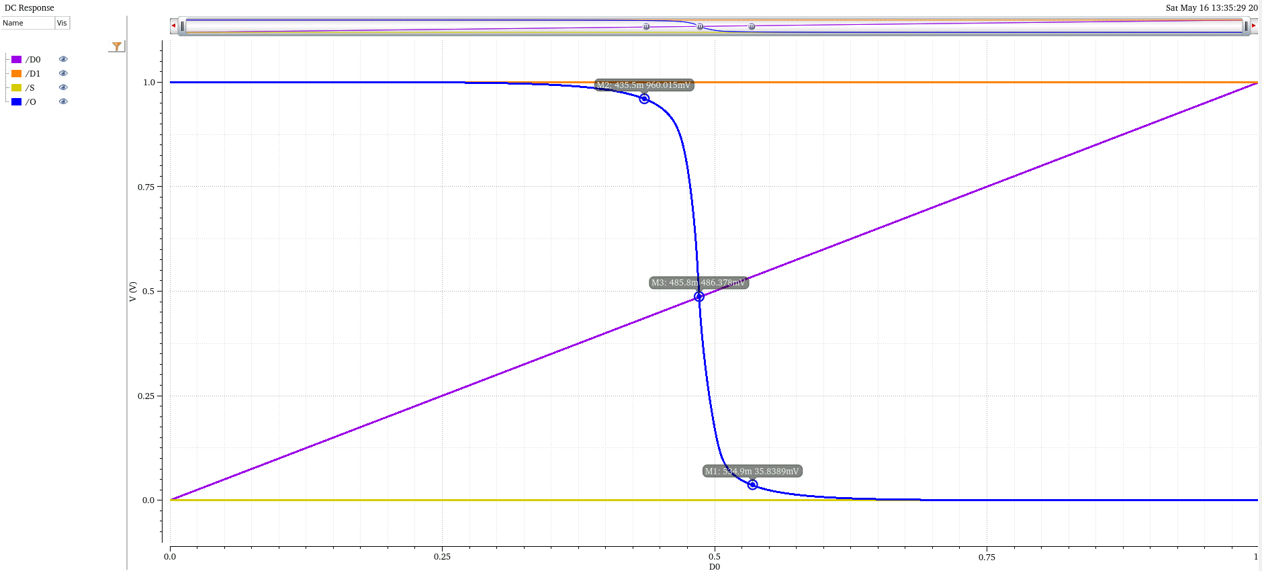
\includegraphics[width=0.6\textwidth]{mux1_dc_sweep_D2.png}}
        \subfigure[DC Sweep TH4]{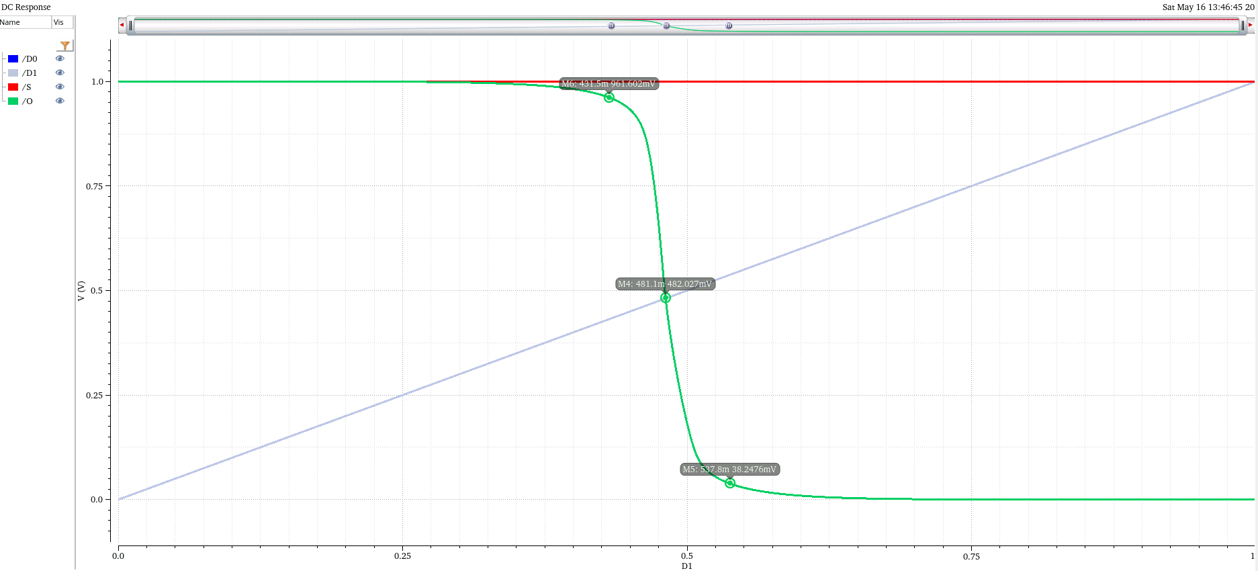
\includegraphics[width=0.6\textwidth]{mux1_dc_sweep_D3.png}}
        \caption{Đặc tuyến VTC của MUX Topology 1 trong các trường hợp khảo sát}
    \end{figure}

    \begin{table}[H]
        \centering
        \caption{Các thông số đặc tính tĩnh DC của mạch MUX Topology 1}
        \begin{tabular}{|c|c|c|c|c|c|c|c|c|}
        \hline
        \textbf{Case} & \textbf{State} & \textbf{$V_{IL}$ (V)} & \textbf{$V_{IH}$ (V)} & \textbf{$V_M$ (V)} & \textbf{$V_{OL}$ (V)} & \textbf{$V_{OH}$ (V)} \\ \hline
        TH1 & Sweep D0 ($S=0, D1=1$) & 0,435 & 0,535 & 0,485 & 0 & 1  \\ \hline
        TH2 & Sweep D0 ($S=1, D1=1$) & 0 & 1 & 0,5 & 0 & 1  \\ \hline
        TH3 & Sweep D1 ($S=0, D0=1$) & 0 & 1 & 0,5 & 0 & 1  \\ \hline
        TH4 & Sweep D1 ($S=1, D0=1$) & 0,432 & 0,538 & 0,481 & 0 & 1  \\ \hline
        \end{tabular}
    \end{table}

    \noindent\textbf{Ghi chú và giải thích các trường hợp khảo sát:}
    \begin{itemize}
        \item \textbf{TH1 \& TH2:} Khi tín hiệu chọn kênh $S$ thay đổi trạng thái logic, đường truyền dẫn từ ngõ vào $D_0$ đến ngõ ra được kích hoạt hoặc khóa, quyết định tính chất nghịch lưu đặc tuyến.
        \item \textbf{TH3 \& TH4:} Đánh giá tương tự khi quét tuyến tính điện áp trên ngõ vào $D_1$. Sự sụt áp qua các cổng truyền (transmission gates) hoặc cấu trúc tĩnh ảnh hưởng đến lề nhiễu logic.
    \end{itemize}

    \item \textbf{Mô phỏng Transient và Đo đạc thông số:}
    \begin{figure}[H]
        \centering
        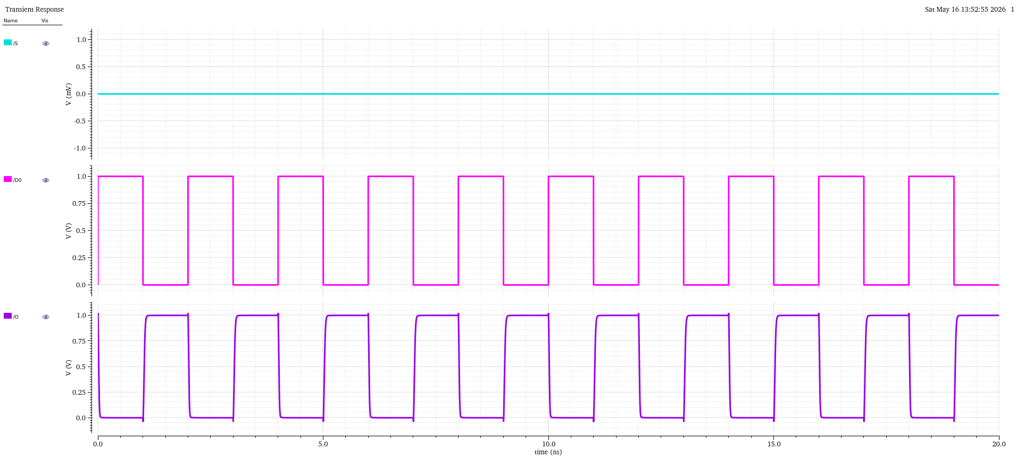
\includegraphics[width=0.8\textwidth]{mux1_transient_waveforms.png}
        \caption{Kết quả mô phỏng Transient MUX Topology 1}
    \end{figure}

    \begin{table}[H]
        \centering
        \caption{Kết quả đo đạc thông số thời gian và công suất bằng Calculator cho MUX 1}
        \begin{tabular}{|c|c|c|c|c|c|c|h|}
        \hline
        \textbf{$t_{rise}$} & \textbf{$t_{fall}$} & \textbf{$t_{pdr}$} & \textbf{$t_{pdf}$} & \textbf{$t_{pd}$} & \textbf{Static Pwr 0} & \textbf{Static Pwr 1} & \textbf{Dynamic Pwr} \\ 
        \textbf{(ps)} & \textbf{(ps)} & \textbf{(ps)} & \textbf{(ps)} & \textbf{(ps)} & \textbf{(nW)} & \textbf{(nW)} & \textbf{($\mu$W)} \\ \hline
        42,82 & 28,93 & 28,85 & 19,27 & 23,66 & 0,35 & ... & 1,21 \\ \hline
        \end{tabular}
    \end{table}

    \begin{figure}[H]
        \centering
        \subfigure[Đo $t_{rise}$]{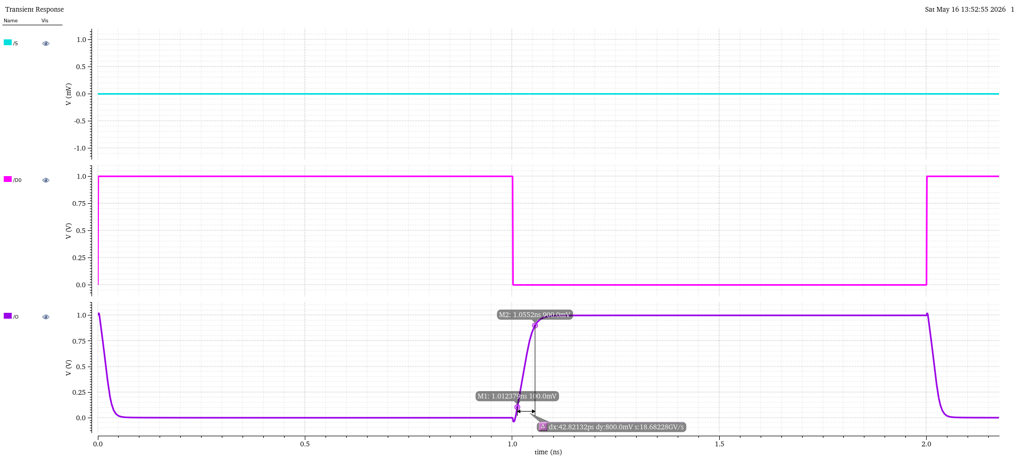
\includegraphics[width=0.5\textwidth]{mux1_trise.png}}
        \subfigure[Calc $t_{rise}$]{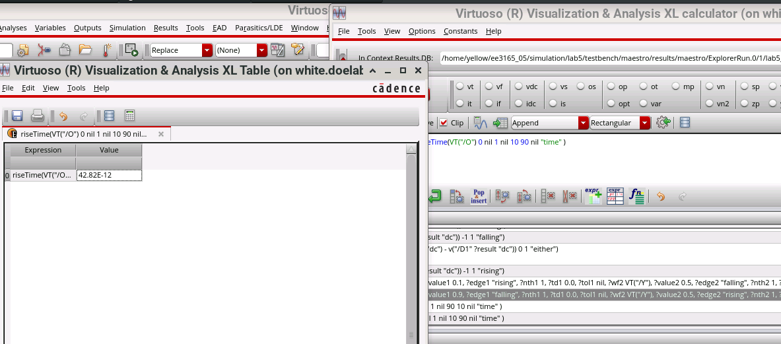
\includegraphics[width=0.5\textwidth]{mux1_trise_calc.png}}
        \subfigure[Đo $t_{fall}$]{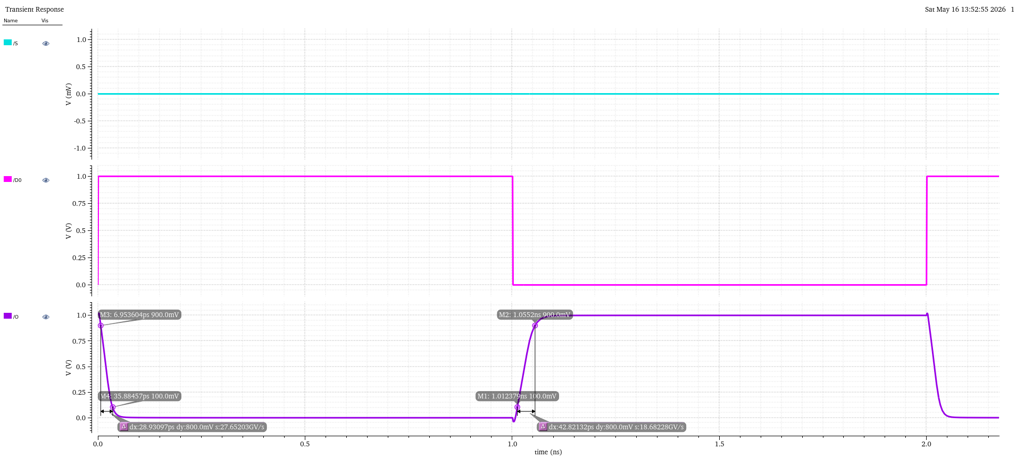
\includegraphics[width=0.5\textwidth]{mux1_tfall.png}}
        \subfigure[Calc $t_{fall}$]{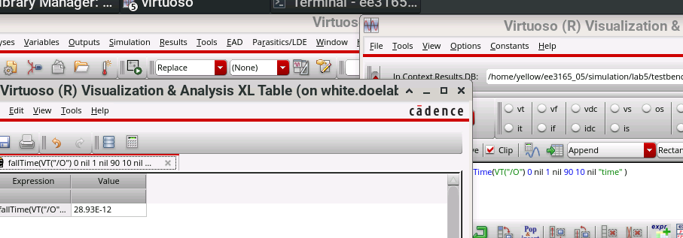
\includegraphics[width=0.5\textwidth]{mux1_tfall_calc.png}}
        \caption{Thời gian cạnh lên và cạnh xuống MUX Topology 1 kèm Calculator}
    \end{figure}
    \begin{figure}[H]
        \centering
        \subfigure[Đo $t_{pdr}$]{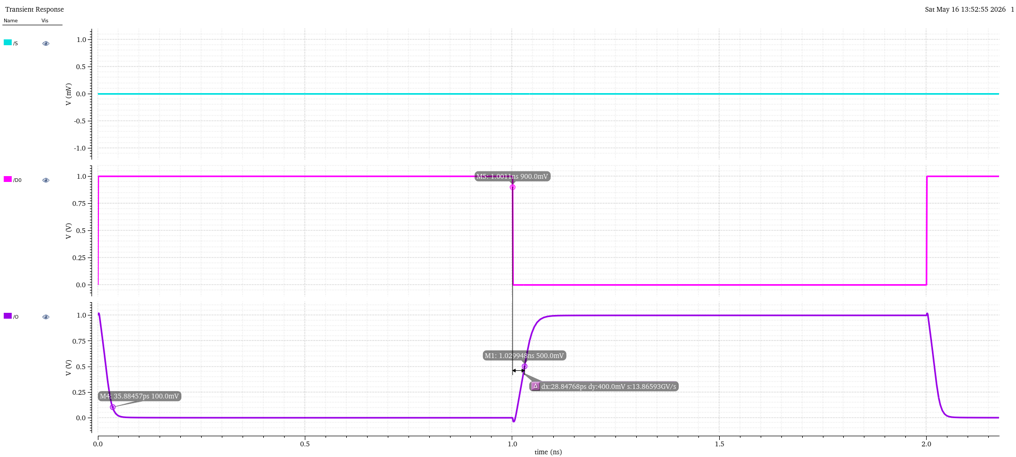
\includegraphics[width=0.5\textwidth]{mux1_tpdr.png}}
        \subfigure[Calc $t_{pdr}$]{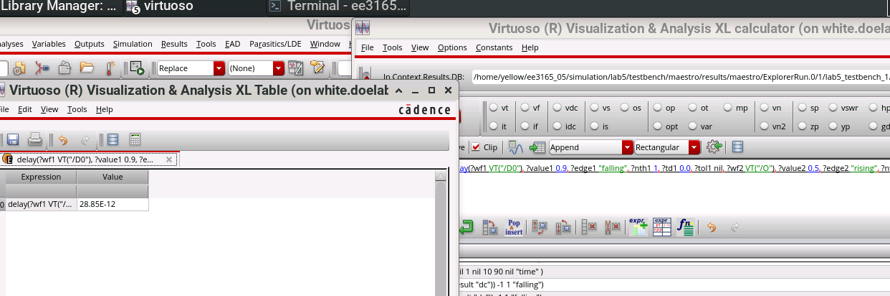
\includegraphics[width=0.5\textwidth]{mux1_tpdr_calc.png}}
        \subfigure[Đo $t_{pdf}$]{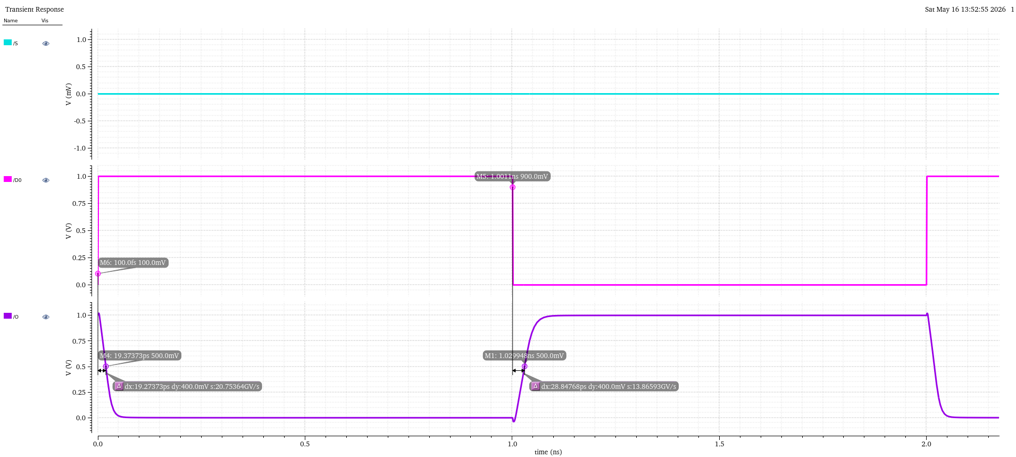
\includegraphics[width=0.5\textwidth]{mux1_tpdf.png}}
        \subfigure[Calc $t_{pdf}$]{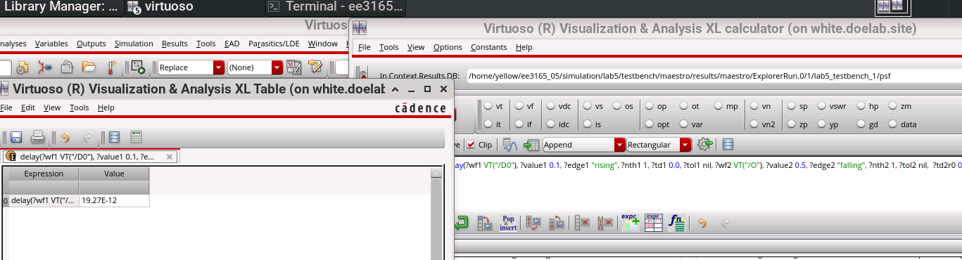
\includegraphics[width=0.5\textwidth]{mux1_tpdf_calc.png}}
        \subfigure[Đo $t_{pd}$]{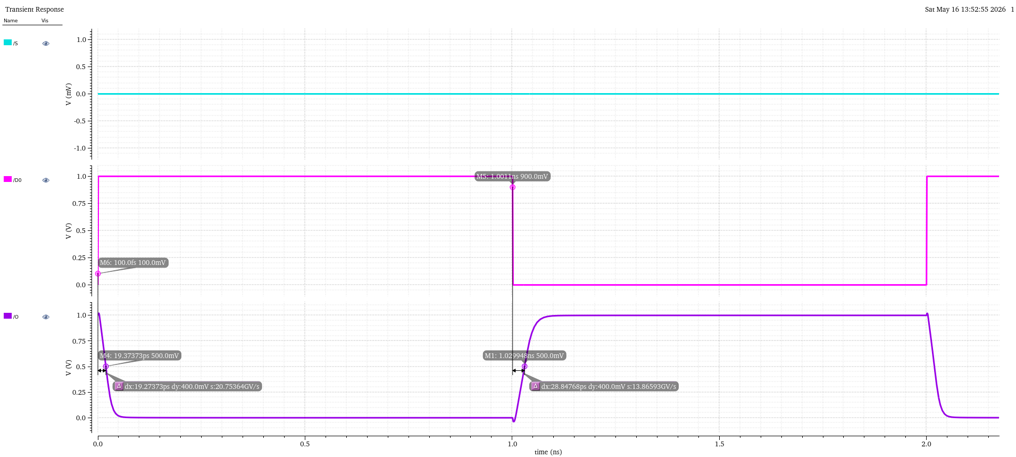
\includegraphics[width=0.52\textwidth]{mux1_tpd.png}}
        \caption{Các thông số độ trễ MUX Topology 1 kèm Calculator}
    \end{figure}
    \begin{figure}[H]
        \centering
        \subfigure[Static Pwr (0)]{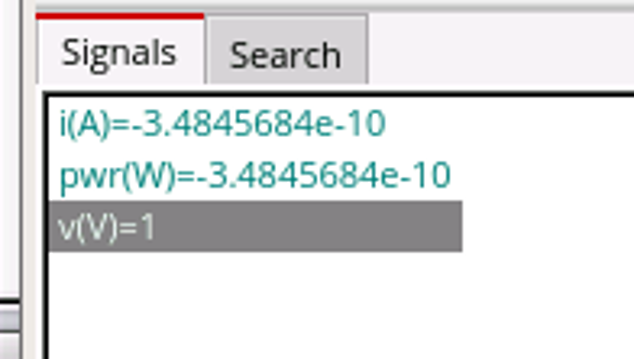
\includegraphics[width=0.5\textwidth]{mux1_static_pwr_0.png}}
        \subfigure[Dynamic Pwr]{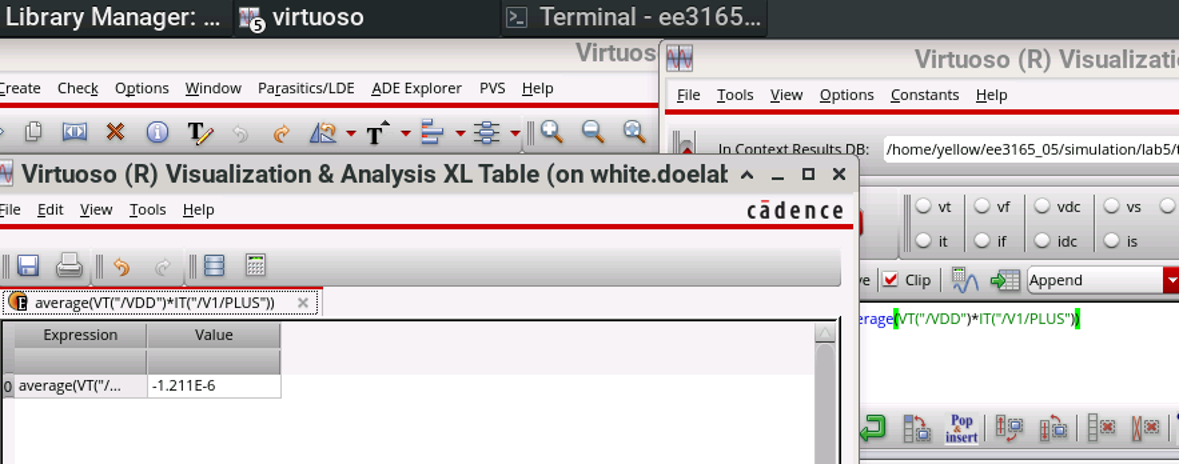
\includegraphics[width=0.6\textwidth]{mux1_dynamic_pwr.png}}
        \caption{Công suất tĩnh và động MUX Topology 1}
    \end{figure}
\end{itemize}
\newpage
\subsection{MUX Topology 2 (MUX Đảo)}
\begin{itemize}
    \item \textbf{Schematic và Symbol:}
    \begin{figure}[H]
        \centering
        \subfigure[Schematic MUX1]{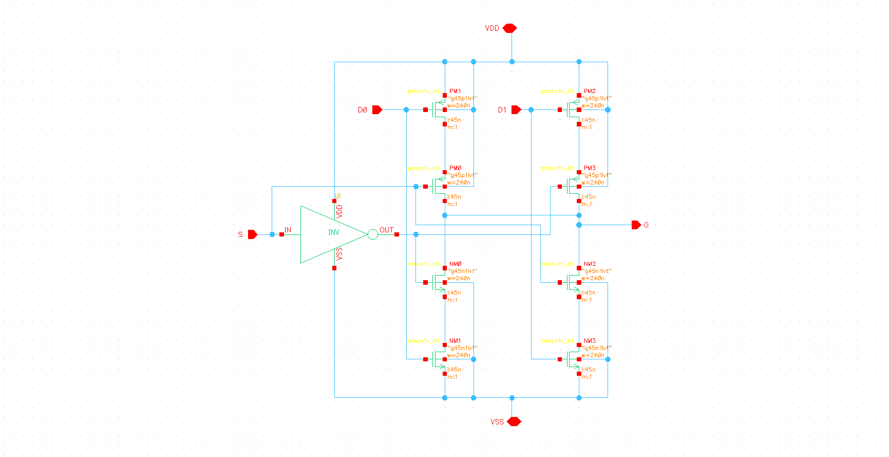
\includegraphics[width=\textwidth]{mux2_schematic.png}}
        \subfigure[Schematic MUX1]{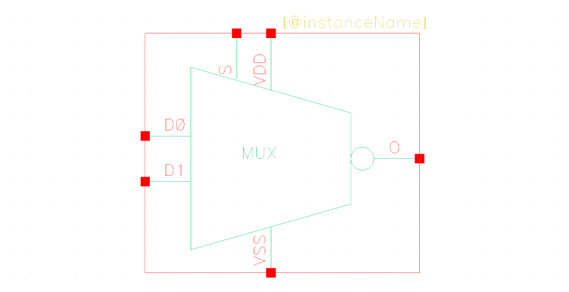
\includegraphics[width=0.6\textwidth]{mux2_symbol.png}}
        \caption{Sơ đồ nguyên lý và Symbol của MUX1}
    \end{figure}
    \item \textbf{Khảo sát DC (4 trường hợp đầy đủ):}
        \begin{enumerate}
            \item TH1: Thay đổi D0 ($S=0, D1=1$).
            \item TH2: Thay đổi D0 ($S=1, D1=1$).
            \item TH3: Thay đổi D1 ($S=0, D0=1$).
            \item TH4: Thay đổi D1 ($S=1, D0=1$).
        \end{enumerate}
    \begin{figure}[H]
        \centering
        \subfigure[DC Sweep TH1]{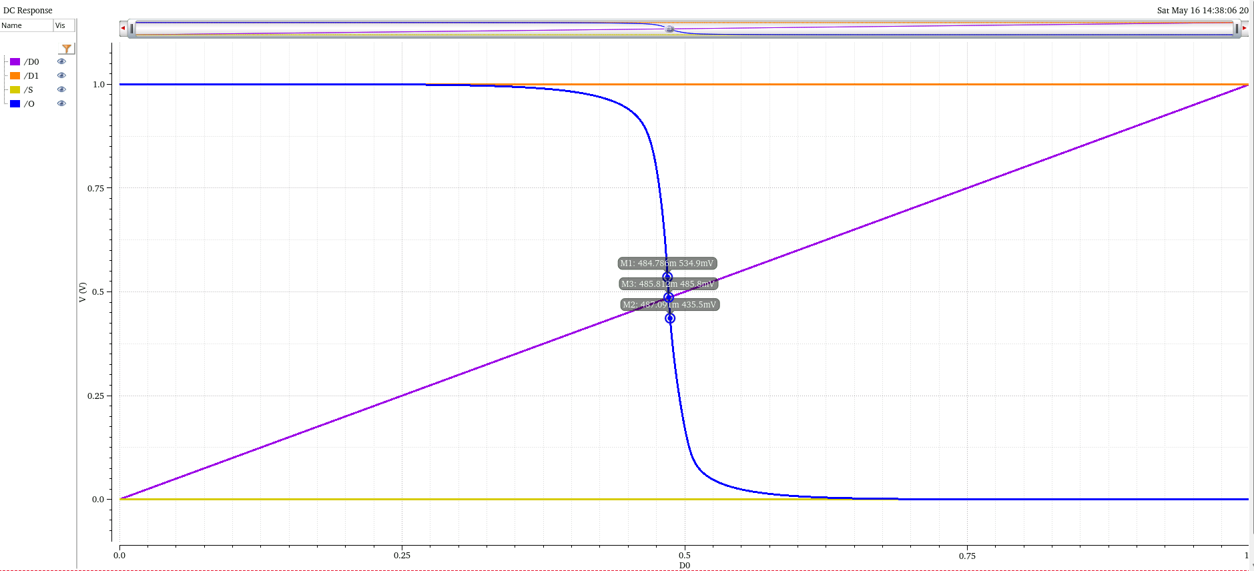
\includegraphics[width=0.6\textwidth]{mux2_dc_sweep_D0.png}}
        \subfigure[DC Sweep TH2]{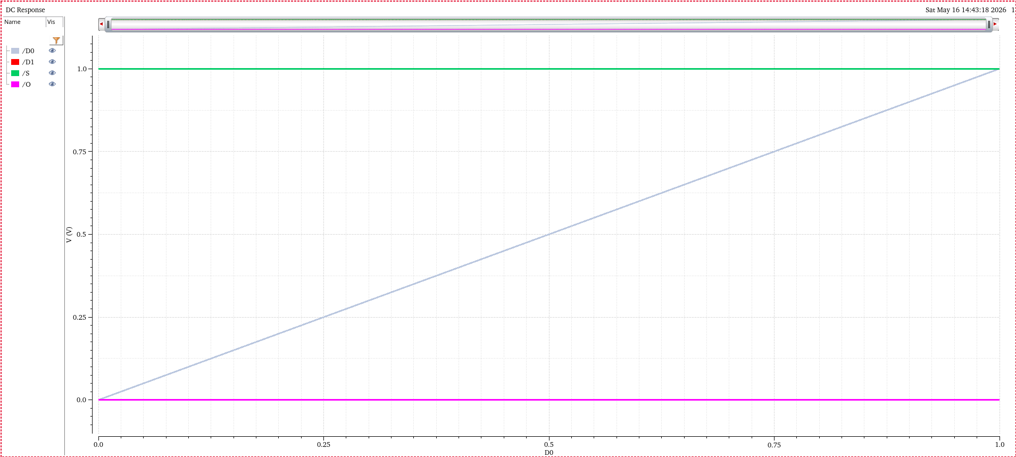
\includegraphics[width=0.6\textwidth]{mux2_dc_sweep_D1.png}}
        \subfigure[DC Sweep TH3]{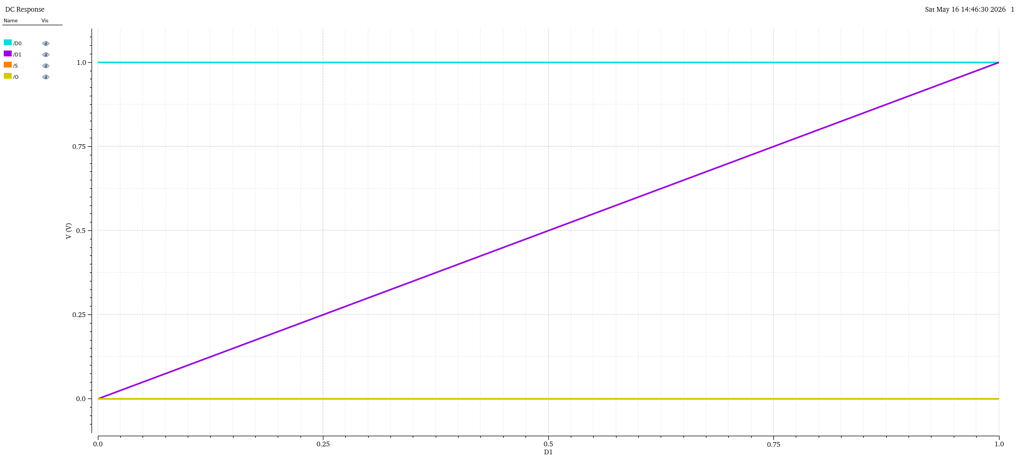
\includegraphics[width=0.6\textwidth]{mux2_dc_sweep_D2.png}}
        \subfigure[DC Sweep TH4]{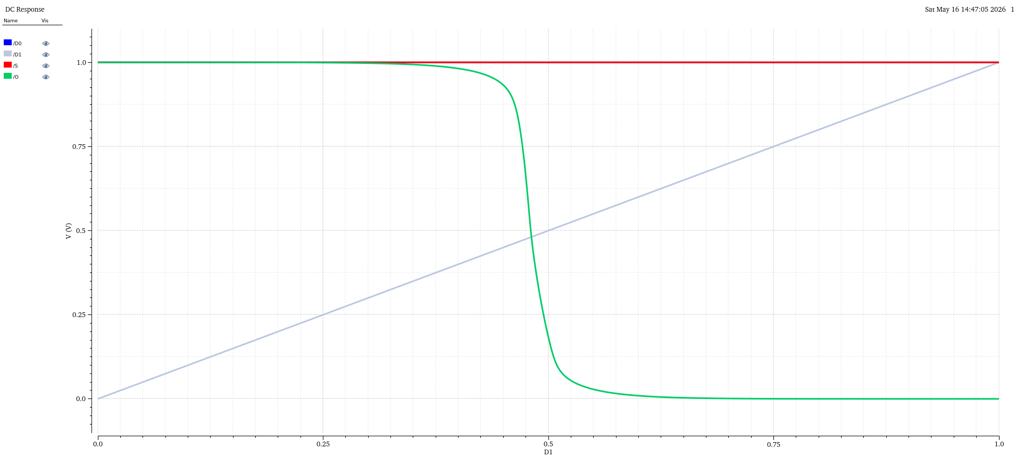
\includegraphics[width=0.6\textwidth]{mux2_dc_sweep_D3.png}}
        \caption{Đặc tuyến VTC của MUX Topology 1 trong các trường hợp khảo sát}
    \end{figure}

    \begin{table}[H]
        \centering
        \caption{Các thông số đặc tính tĩnh DC của mạch MUX Topology 2}
        \begin{tabular}{|c|c|c|c|c|c|c|c|c|}
        \hline
        \textbf{Case} & \textbf{State} & \textbf{$V_{IL}$ (V)} & \textbf{$V_{IH}$ (V)} & \textbf{$V_M$ (V)} & \textbf{$V_{OL}$ (V)} & \textbf{$V_{OH}$ (V)}\\ \hline
        TH1 & Sweep D0 ($S=0, D1=1$) & 0,4 & 0,5 & 0,6 & 0 & 1 &  \\ \hline
        TH2 & Sweep D0 ($S=1, D1=1$) & 0 & 1 & 0,5 & 0 & 1 &  \\ \hline
        TH3 & Sweep D1 ($S=0, D0=1$) & 0 & 1 & 0,5 & 0 & 1 &  \\ \hline
        TH4 & Sweep D1 ($S=1, D0=1$) & 0,4 & 0,5 & 0,6 & 0 & 1 &  \\ \hline
        \end{tabular}
    \end{table}

    \noindent\textbf{Ghi chú và giải thích các trường hợp khảo sát:}
    \begin{itemize}
        \item \textbf{TH1 \& TH2:} Khảo sát đặc tính chuyển mạch tĩnh theo ngõ vào $D_0$ đối với cấu trúc cấu thành thứ hai, theo dõi sụt áp nút nội tại.
        \item \textbf{TH3 \& TH4:} Đánh giá hoạt động tĩnh dựa trên sự biến thiên mức điện áp ngõ vào $D_1$, phân tích độ đối xứng lề nhiễu logic cao và logic thấp.
    \end{itemize}

    \item \textbf{Mô phỏng Transient và Đo đạc thông số:}
    \begin{figure}[H]
        \centering
        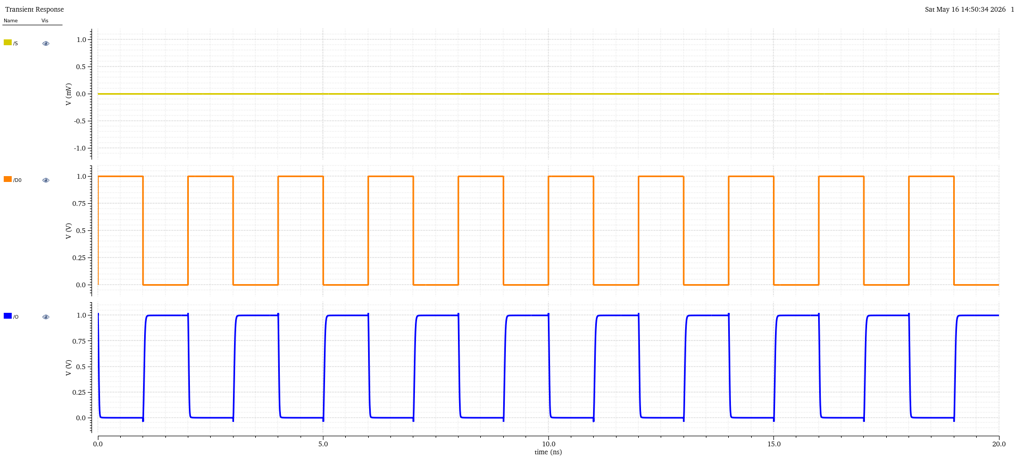
\includegraphics[width=0.8\textwidth]{mux2_transient_waveforms.png}
        \caption{Kết quả mô phỏng Transient MUX Topology 2}
    \end{figure}

    \begin{table}[H]
        \centering
        \caption{Kết quả đo đạc thông số thời gian và công suất bằng Calculator cho MUX 2}
        \begin{tabular}{|c|c|c|c|c|c|c|h|}
        \hline
        \textbf{$t_{rise}$} & \textbf{$t_{fall}$} & \textbf{$t_{pdr}$} & \textbf{$t_{pdf}$} & \textbf{$t_{pd}$} & \textbf{Static Pwr 0} & \textbf{Static Pwr 1} & \textbf{Dynamic Pwr} \\ 
        \textbf{(ps)} & \textbf{(ps)} & \textbf{(ps)} & \textbf{(ps)} & \textbf{(ps)} & \textbf{(nW)} & \textbf{(nW)} & \textbf{($\mu$W)} \\ \hline
        42,82 & 28,93 & 28,85 & 19,27 & 23,66 & 0,35 & ... & 1,21 \\ \hline
        \end{tabular}
    \end{table}

    \begin{figure}[H]
        \centering
        \subfigure[Đo $t_{rise}$]{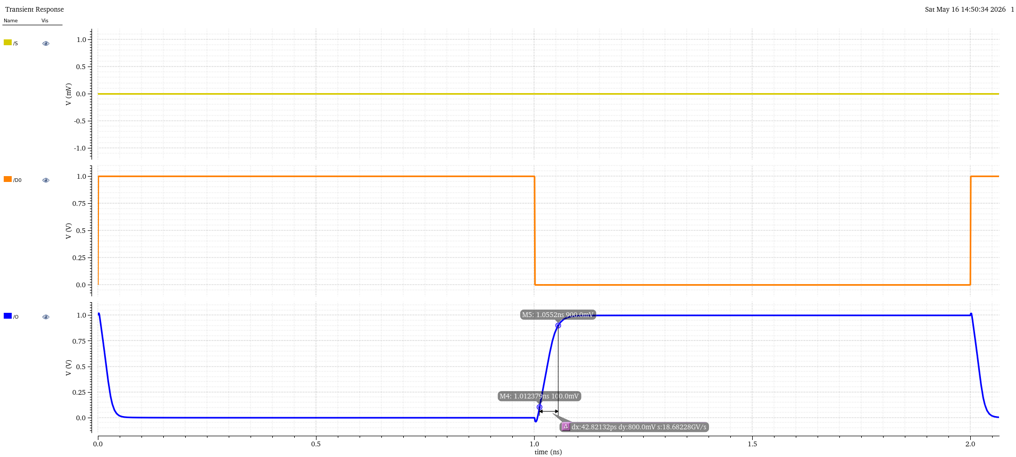
\includegraphics[width=0.5\textwidth]{mux2_trise.png}}
        \subfigure[Calc $t_{rise}$]{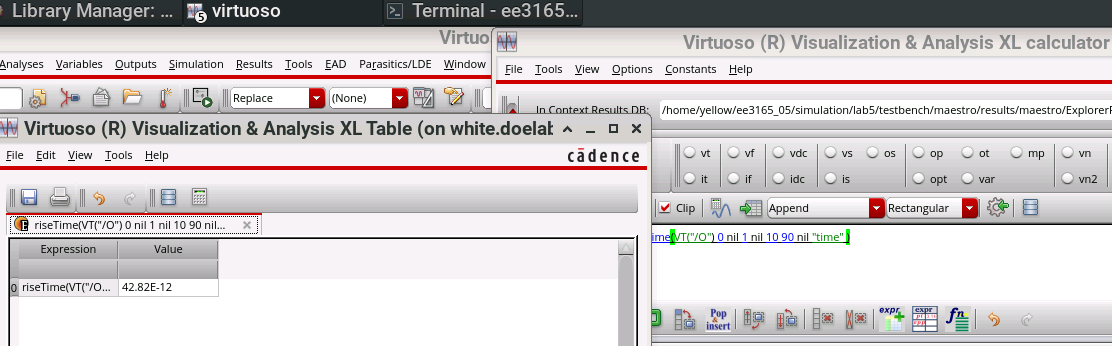
\includegraphics[width=0.5\textwidth]{mux2_trise_calc.png}}
        \subfigure[Đo $t_{fall}$]{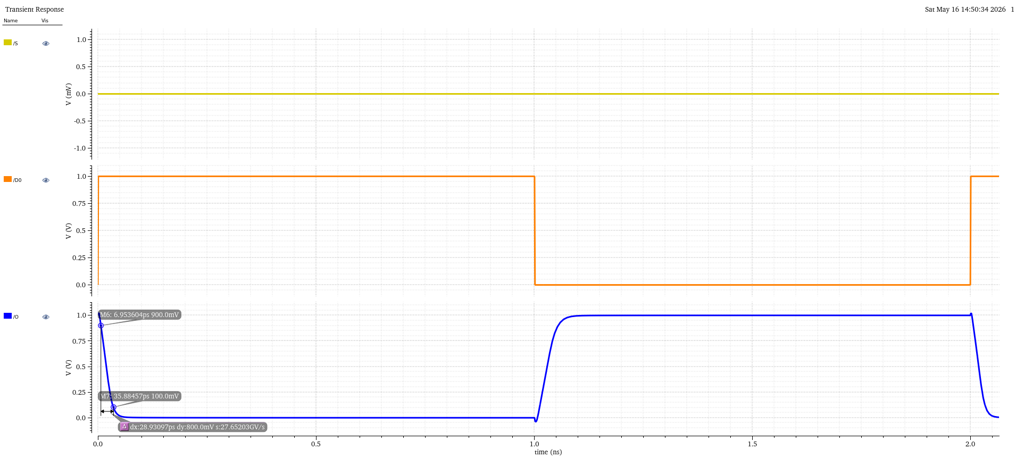
\includegraphics[width=0.5\textwidth]{mux2_tfall.png}}
        \subfigure[Calc $t_{fall}$]{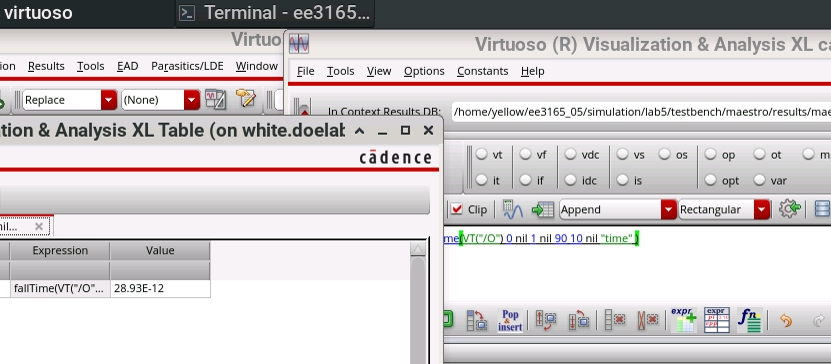
\includegraphics[width=0.5\textwidth]{mux2_tfall_calc.png}}
        \caption{Thời gian cạnh lên và cạnh xuống MUX Topology 2 kèm Calculator}
    \end{figure}
    \begin{figure}[H]
        \centering
        \subfigure[Đo $t_{pdr}$]{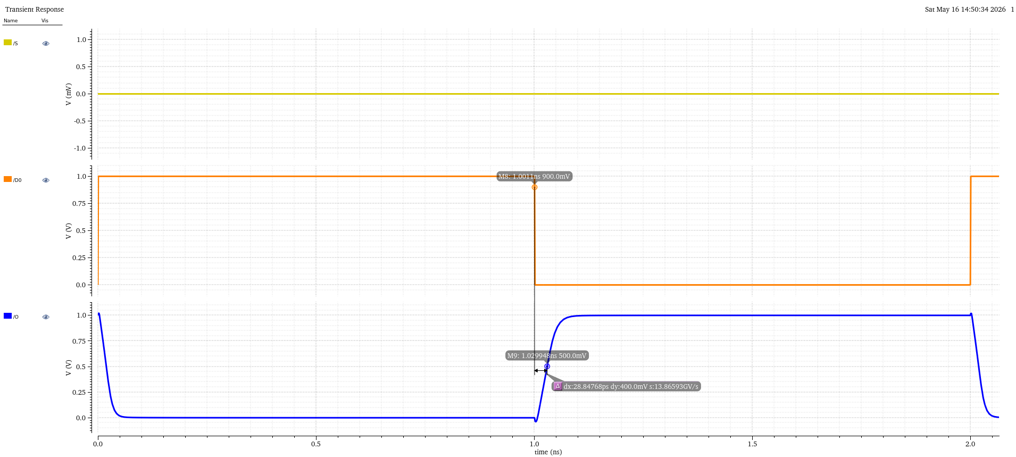
\includegraphics[width=0.5\textwidth]{mux2_tpdr.png}}
        \subfigure[Calc $t_{pdr}$]{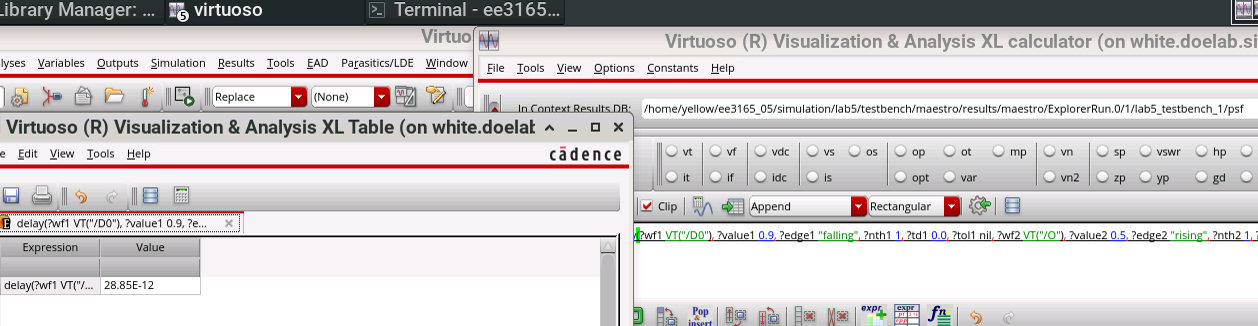
\includegraphics[width=0.5\textwidth]{mux2_tpdr_calc.png}}
        \subfigure[Đo $t_{pdf}$]{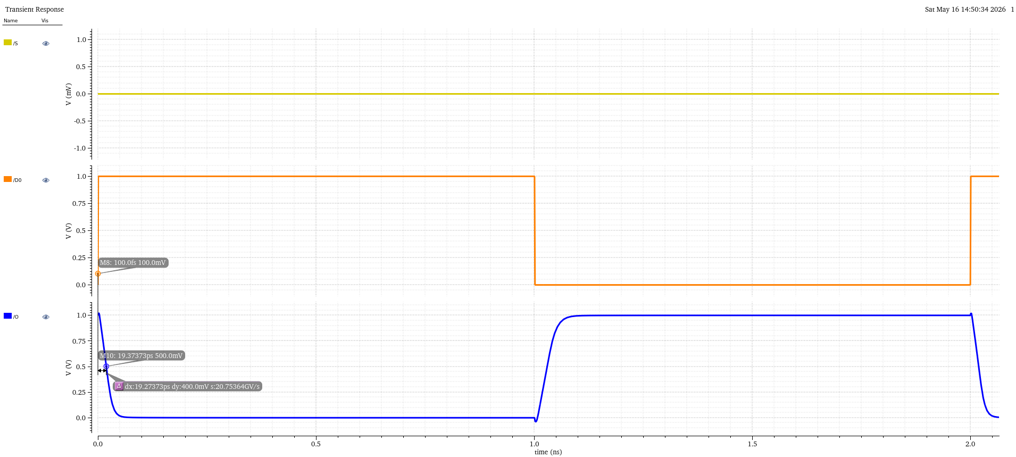
\includegraphics[width=0.5\textwidth]{mux2_tpdf.png}}
        \subfigure[Calc $t_{pdf}$]{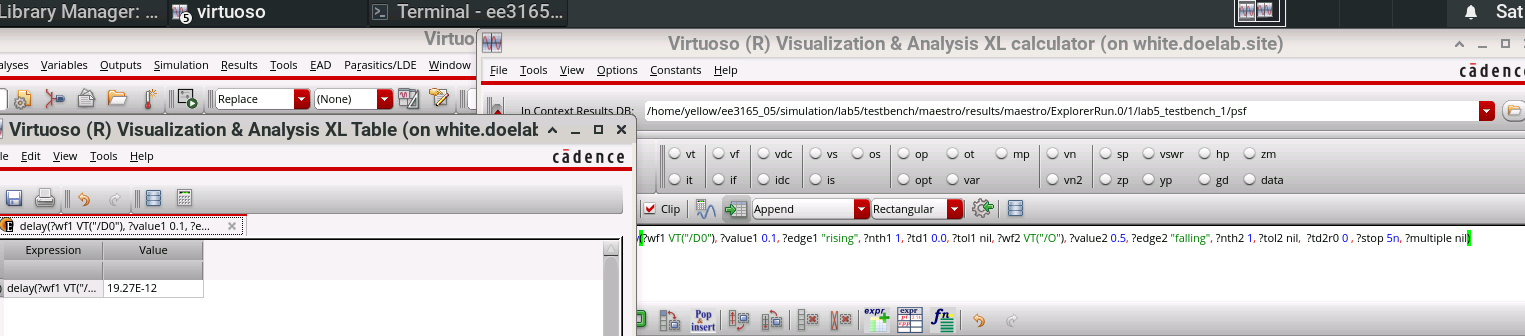
\includegraphics[width=0.5\textwidth]{mux2_tpdf_calc.png}}
        \subfigure[Đo $t_{pd}$]{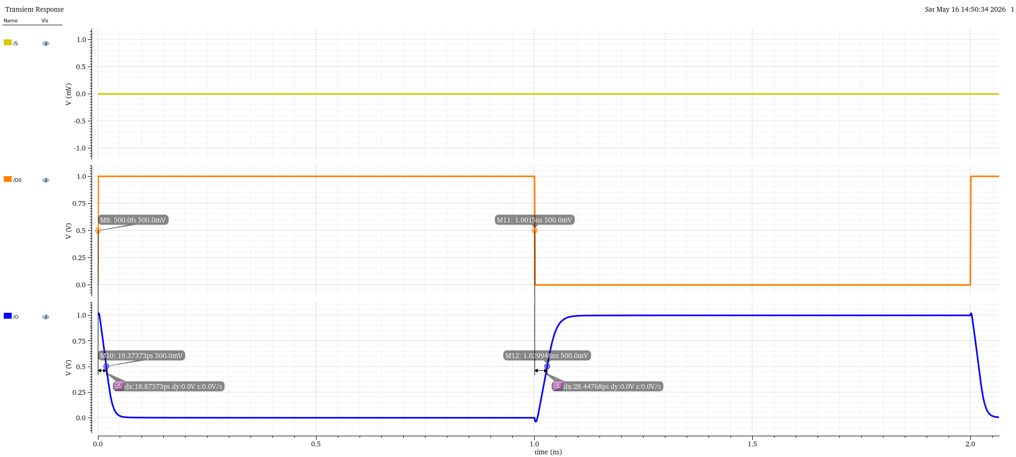
\includegraphics[width=0.5\textwidth]{mux2_tpd.png}}
        \caption{Các thông số độ trễ MUX Topology 2 kèm Calculator}
    \end{figure}
    \begin{figure}[H]
        \centering
        \subfigure[Static Pwr (0)]{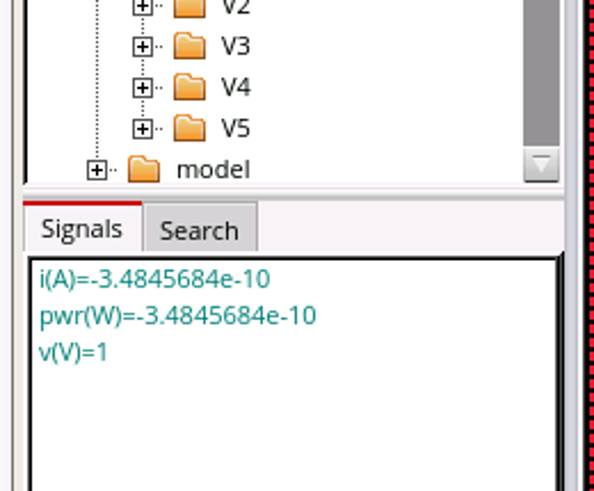
\includegraphics[width=0.5\textwidth]{mux2_static_pwr_0.png}}

        \subfigure[Dynamic Pwr]{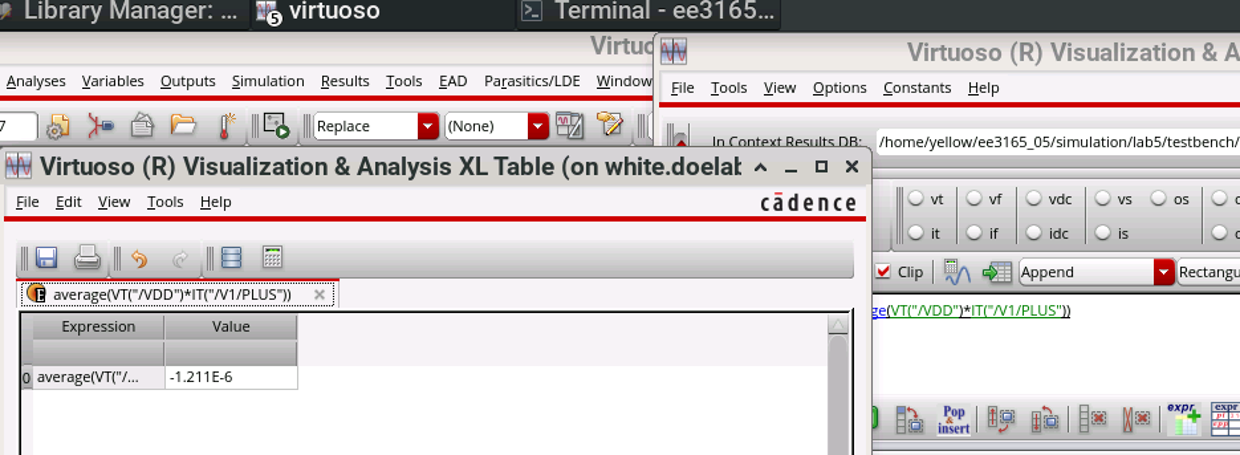
\includegraphics[width=0.5\textwidth]{mux2_dynamic_pwr.png}}
        \caption{Công suất tĩnh và động MUX Topology 2}
    \end{figure}

\end{itemize}

\subsection{So sánh và đánh giá hai kiến trúc mạch MUX}

Dựa trên các kết quả mô phỏng đặc tính tĩnh và đặc tính động đã đo đạc ở hai phần trước, cùng với nguyên lý hoạt động nội tại của từng cấu trúc tế bào tiêu chuẩn, ta có thể lập bảng tổng hợp định lượng và đưa ra các đánh giá định tính cho hai kiến trúc MUX Đảo như sau:

\subsubsection{Phân tích chuyên sâu về sự khác biệt giữa hai kiến trúc}
Thông thường trong thiết kế Standard Cell, hai kiến trúc phổ biến nhất để hiện thực MUX là cấu trúc cổng logic CMOS tĩnh và cấu trúc dùng cổng truyền dẫn. Sự khác biệt về số đo giữa hai Topology bắt nguồn từ chính bản chất vật lý của chúng:

\begin{itemize}
    \item \textbf{Về cấu trúc và Diện tích:} 
    Topology sử dụng logic CMOS tĩnh truyền thống đòi hỏi việc xây dựng mạng kéo lên (PUN) bằng PMOS và mạng kéo xuống (PDN) bằng NMOS bù trừ hoàn toàn. Điều này khiến cấu trúc trở nên cồng kềnh, tiêu tốn nhiều transistor (thường từ 10-12 transistor), làm tăng diện tích vật lý chiếm dụng trên tấm Silicon. Ngược lại, Topology áp dụng kỹ thuật cổng truyền (TG) tận dụng đặc tính truyền dẫn tín hiệu trực tiếp của cặp NMOS-PMOS mắc song song. Nó đóng vai trò như các công tắc điện tử lý tưởng, giúp giảm đáng kể số lượng bóng bán dẫn xuống chỉ còn 6-8 transistor, tối ưu hóa đáng kể mật độ tích hợp mạch.

    \item \textbf{Về đặc tính thời gian định thời:}
    Nhờ đường truyền dẫn trực tiếp, tín hiệu dữ liệu ($D_0, D_1$) trong kiến trúc TG có thể đi thẳng qua cổng truyền đến ngõ vào của tầng nghịch lưu cuối cùng mà không phải tuần tự đi qua nhiều tầng cổng logic cơ bản. Do đó, nếu tính riêng đường trễ từ ngõ vào dữ liệu tới ngõ ra, cấu trúc TG thường cho tốc độ đáp ứng nhanh hơn, cạnh xung dốc hơn và độ trễ $t_{pd}$ thấp hơn. Tuy nhiên, kiến trúc CMOS tĩnh tuy có đường trễ tới hạn dài hơn do cấu trúc mạng nối tiếp/song song, nhưng lại đem lại độ ổn định thời gian rất tốt, ít nhạy cảm với sự biến đổi của điện trở đầu vào.

    \item \textbf{Về điện năng tiêu thụ:}
    Công suất động của mạch số tỉ lệ thuận với tổng điện dung tải chuyển mạch ($P_{dyn} \propto C_{load} \cdot V_{DD}^2 \cdot f$). Cấu trúc CMOS tĩnh chứa nhiều transistor và nhiều nút nối nội bộ (internal nodes) hơn, sinh ra dung kháng ký sinh lớn. Hệ quả tất yếu là nó sẽ tiêu tốn nhiều năng lượng dạng động hơn trong mỗi chu kỳ đóng cắt. Cấu trúc TG giúp triệt tiêu bớt các nút nội bộ nên tiết kiệm điện năng hơn, nhưng đổi lại, tín hiệu điều khiển kênh ($S$ và $\overline{S}$) yêu cầu phải được cung cấp đồng thời và hoàn toàn đối xứng. Sự lệch pha (skew) giữa hai tín hiệu điều khiển này có thể gây ra hiện tượng chập mạch chớp nhoáng, sinh ra các gai công suất ngoài ý muốn.

    \item \textbf{Về khả năng lái tải và Phục hồi logic:}
    Các cổng CMOS tĩnh luôn luôn có cấu trúc kết nối ngõ ra trực tiếp đến dải nguồn $V_{DD}$ hoặc $GND$, do đó chúng cung cấp dòng xả/nạp rất mạnh và biên độ điện áp luôn đạt mức đầy đủ. Ngược lại, tín hiệu đi qua hệ thống Transmission Gate có hiện tượng tích lũy nội trở kênh dẫn, dẫn đến tốc độ Slew-rate có xu hướng bị suy giảm khi tải lớn. Việc thiết kế tầng đệm tại ngõ ra của cả hai Topology là bắt buộc để khôi phục mức logic sắc nét và đảm bảo năng lực đẩy dòng cho các tầng mạch số phía sau.
\end{itemize}

\textbf{Kết luận phần MUX:} 
Việc lựa chọn Topology nào phụ thuộc hoàn toàn vào bài toán thiết kế cụ thể: Nếu ưu tiên tối đa hóa diện tích và tiết kiệm năng lượng, Topology dùng cổng truyền dẫn (Transmission Gate) là giải pháp hoàn hảo; ngược lại, nếu cần độ ổn định logic tuyệt đối và khả năng lái tải ưu việt trong môi trường nhiễu cao, Topology CMOS tĩnh sẽ được ưu tiên sử dụng.


\end{document}